%\documentclass[10pt,a4paper]{article}
\documentclass[12pt,a4paper]{article}
\usepackage{graphicx,units,amsmath}
\usepackage{bm} % bold in math mode
\usepackage{subfigure}
\usepackage{float}
\usepackage[ngerman, english]{babel} 
%\usepackage[utf8]{inputenc}
\setcounter{secnumdepth}{4}

\usepackage[top=2cm, bottom=2.5cm, left=3cm, right=3cm]{geometry}

%-Eingabe der Metadaten des Titelblattes--------------------------

%-Daten des Autors / Authors Data---------------------------------

\newcommand{\dcauthorpre}{~} 
\newcommand{\dcauthorsurname}{Kullmann} 
\newcommand{\dcauthorname}{Richard} 
\newcommand{\dcauthoradd}{geboren am 17.07.1996 in Berlin-Pankow}

%-Titel und Untertitel / Title and subtitle-----------------------

\newcommand{\dctitle}{Giant Diffusion in two-dimensional Neuron Models} 
\newcommand{\dcsubtitle}{~}  
% Falls dcsubtitle NICHT verwendet werden soll, {\dcsubtitle}{~} eingeben.

%-Eingabe der Betreuuernahmen / Names of the consultants---------

\newcommand{\dcconsulta}{~} 
\newcommand{\dcconsultb}{~} 
\newcommand{\dcconsultc}{~} 

%-Eingabe der Gutachternamen / Names of the approvals-------------

\newcommand{\dcapprovala}{Prof. Dr. Benjamin Lindner} 
\newcommand{\dcapprovalb}{Prof. Dr. Igor Sokolov} 
\newcommand{\dcapprovalc}{~} 

%-Information zur Universitaet------------------------------------

\newcommand{\dcdegree}{Master of Science\\(M. Sc.)} 
\newcommand{\dcsubject}{Physik} 
\newcommand{\dcfaculty}{Mathematisch-Naturwissenschaftlichen Fakult\"at I}
\newcommand{\dcinstitute}{Institut f\"ur Physik}
\newcommand{\dcuniversity}{Humboldt-Universit\"at zu Berlin}
\newcommand{\dcdean}{Prof. Dr. sc. Heinz  M\"uller}
\newcommand{\dcpresident}{Prof. Dr. Dr. h.c. Wilhelm Schulz}

%-Pruefungsdaten: eingereicht und mdl. Pruefung-------------------
%-data of submission and oral exam--------------------------------

\newcommand{\dcdatesubmitted}{5. Juni 2020} %auch wenn nicht auf dem 
%Titelblatt, bitte erf�llen!
\newcommand{\dcdateexam}{2. Juli 1999} 


% Folgende Zeile bitte nicht aendern!
\newcommand{\dckeywordsde}{\vfill \raggedright {\textbf{Schlagw\"orter:}}\\ \dckeydea, \dckeydeb, \dckeydec, \dckeyded \\}

%-englische Schlagwoerter / english keywords----------------------

\newcommand{\dckeyena}{Giant Diffusion}
\newcommand{\dckeyenb}{Two-Dimensional Neuron Models}
\newcommand{\dckeyenc}{Bistability}
\newcommand{\dckeyend}{Signal-to-Noise Ratio}

% Folgende Zeile bitte nicht aendern!
\newcommand{\dckeywordsen}{\vfill \raggedright {\textbf{Keywords:}}\\ \dckeyena, \dckeyenb, \dckeyenc, \dckeyend \\}

\newcommand{\dcpdfsubject}{Dissertation}  
\graphicspath{{images/}}
\begin{document}


%\title{Masterarbeit}
%\author{Richard Kullmann}
%\date{15.07.2019}

%----------Generierung der Titelseite-----bitte nicht ver�ndern!--------------------


\author{von \\ \dcauthorpre\ \dcauthorname\ \dcauthorsurname\ \\ \dcauthoradd}

%----------
\title{ \vspace{-2cm}\dctitle \\ 
\vspace{0.5cm}
\large{\dcsubtitle} \\ 
\vspace{0.5cm} {\Large{MASTERARBEIT}}\\ 
\vspace{0.5cm} \large{zur Erlangung des akademischen Grades \\ 
\dcdegree\\ im Fach \dcsubject \\\vspace{0.5cm}

\includegraphics[width=6cm]{husiegel}\\ 
\vspace{0.5cm} eingereicht an der \\ 
\dcfaculty \\ 
\dcinstitute\\
\dcuniversity \\}}
%-----------------
\date{\vspace{2.5cm}
%\raggedright{
%Pr\"asident der Humboldt-Universit\"at zu Berlin:\\
%\dcpresident \vspace{-0.3cm}
%}\vspace{0.5cm}\\
%
%\raggedright{
%Dekan der \dcfaculty:\\
%\dcdean \vspace{-0.3cm}
%}\vspace{0.5cm}\\
%
% auskommentiert weil nicht standard
\raggedright{
Gutachter:
\begin{enumerate} 
\item{\it\dcapprovala} \vspace{-0.3cm}
\item{\it\dcapprovalb} \vspace{-0.3cm}
%\item{\it\dcapprovalc} \vspace{-0.3cm}
\end{enumerate}} \vspace{0.5cm}
%\raggedright{
%Betreuung:
%\begin{enumerate} 
%\item{\it\dcconsulta} \vspace{-0.2cm}
%\item{\it\dcconsultb} \vspace{-0.2cm}
%\end{enumerate}} \vspace{0.5cm}
%-----------------
\raggedright{
\begin{tabular}{lll}
eingereicht am: &  &\it\dcdatesubmitted\\ % wenn nicht in der Pr�fungsordnung, die Zeile bitte auskommentieren
%Tag der m\"undlichen Pr\"ufung: & & \dcdateexam
\end{tabular}}\\ 
}
%------------------------------------- 

\maketitle

\thispagestyle{empty}
%\setcounter{page}{2}
\newpage
%-englische-Zusammenfassung---------------------------------------

%\selectlanguage{english}

%\begin{abstract}
%\setcounter{page}{2} % Nach Bedarf anpassen!
%Here is the english abstract.\\
% hier werden die englische Schlagw�rter aus Metadaten �bernommen
%\dckeywordsen				
%\end{abstract}

%-deutsche Zusammenfassung----------------------------------------

%\selectlanguage{german}

\begin{abstract}
\setcounter{page}{2} % Nach Bedarf anpassen!
The emerging field of magnetometry based on NV centers opens a variety of new experimental perspectives, including the imaging of single nuclear spins on the nanoscale. However, in order to achieve exceptionally long NV electron spin coherence times and high sensitivities, the NV spin needs to be decoupled from unwanted interactions with the environment. This can be accomplished with dynamical decoupling sequences.
\\
During the work for this thesis, multiple dynamical decoupling protocols were implemented and tested on NV centers in bulk diamond and nanodiamond. 
\\
The theoretical part covers general NV properties before treating the behaviour of a free electron spin and finally applying this on the NV center. Then, the effect of different decoupling protocols are discussed. After that, the structure and concept of the setup will be explained. In the final part, the measurements will be presented. The execution of the decoupling sequences will be demonstrated and the data will be used to extract the spectral density function of the environment.
\\
It was shown that all implemented dynamical decoupling sequences could enhance the coherence time. It was demonstrated that CPMG outperforms the other sequences on the given setup, achieving an improvement of up to a factor of 200 in the bulk diamond and 50 in nanodiamond. Finally, the examination of the spectral density functions of the spin bath gave a deeper insight in its coupling strength to the NV and its internal dynamics.\\
In the future, the limitations of the sequences will be further explored and other decoupling protocols will be tested. In addition to that, a better time and phase control has to be accomplished. These efforts will eventually lead to sensitivities high enough to detect small spin ensembles and even single molecular spins.
% hier werden die deutsche Schlagw�rter aus Metadaten �bernommen
%\dckeywordsde
\end{abstract}
\thispagestyle{empty}

\tableofcontents
\thispagestyle{empty}
\newpage
\pagenumbering{arabic}

\section{Introduction}

The human brain is one of the most investigated but still least understood subjects in scientific research. This comes as no surprise considering the huge variety of tasks it can perform efficiently and seemingly effortlessly: it constantly combines multiple sensory impressions and filters the most relevant of them to form a coherent image of the surroundings, it remembers information it has learned decades ago, it can produce the most complex thoughts and keep a whole organism working properly in the meantime. And despite the mayor improvement of processor performance and increasing interest in machine learning and artificial neural networks during the past couple of years, no technological implementation has even remotely managed to match the capability of the human brain.\\
The basis for its high functionality lies in the huge number of neurons - around 100 Billions\cite{eqnum} - and their interconnectivity: neural cells usually receive inputs from more than 10.000 other neurons\cite{izi}. Thus, in order to be able to understand how the brain works and possibly derive future applications from that, it is crucial to examine neural cells and study their characteristics. \\
Information in neurons is mainly transmitted via spikes. A spike is an abrupt change of membrane voltage that propagates through the axon. Neural cells do not only produce spikes but display a plethora of responses to their synaptic inputs. In general, neural activity can be divided into four mayor regimes: resting state, sub-threshold oscillations, spiking and bursting\cite{dnb}. During resting-state and sub-threshold oscillations, the neuron does not spike, a spiking neuron fires spikes in regular intervals and a bursting neuron produces multiple spikes followed by periods of quiescence. Often, multiple of these regimes can be found in a single neuron. Of particular interest is the bistability between resting and spiking activity. This has been observed in pacemaker\cite{pacemaker}, sensory \cite{sensory}\cite{sensorystm1} and motoneurons\cite{moto1}\cite{moto2} and is suggested to play important roles in short term memory and processing\cite{sensorystm1}\cite{stm1}\cite{stm2} as well as in shaping patterns of so-called spindle oscillations\cite{spindle}. Some experimental data of bistable neurons are shown in figure \ref{expbistable}.
\begin{figure}[H]
	\subfigure[]{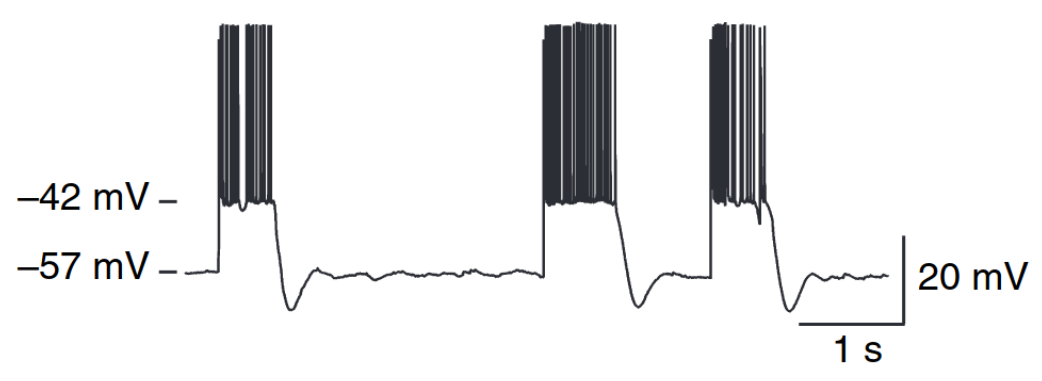
\includegraphics[width=0.6\textwidth]{bistableloewenstein.png}} 
	\subfigure[]{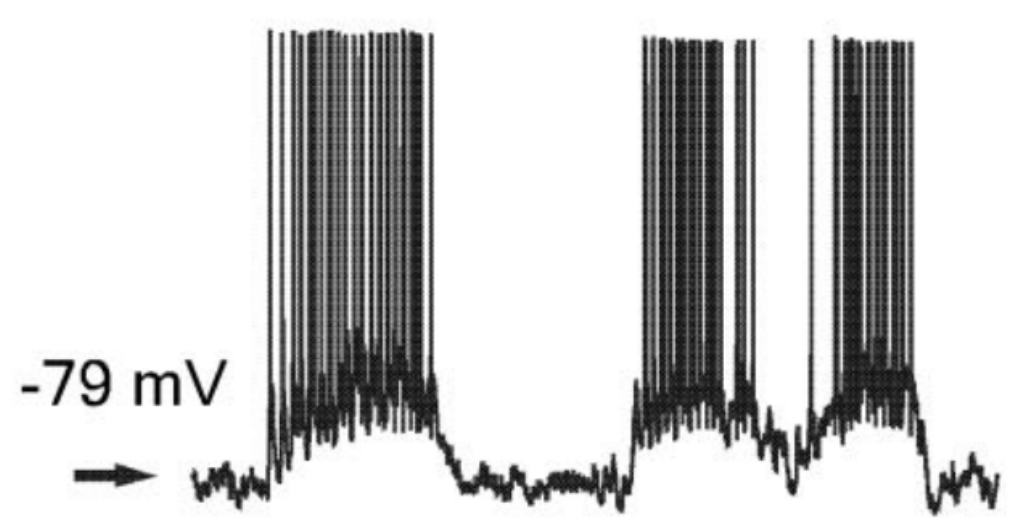
\includegraphics[width=0.4\textwidth]{bistablespindle2.png}} 
	\caption{Experimental observation of neural bistability. On the left side, recordings of rat Purkinje cells are shown\cite{sensorystm1} and the right image was obtained from cat RE neurons\cite{spindle}}
	\label{expbistable} 
\end{figure}
As each regime displays different voltage dynamics, a bistability in neural activity directly translates into a bistability of the membrane voltage. When noise is added to the system, stochastic switchings between the states will occur. That way, the bistable system is turned into a stochastically bursting neuron model. If the influence of the noise is small in comparison to the other ionic currents, the membrane voltage takes on a rectangular shape. In the resting state, the voltage performs noise-driven oscillations around the stable equilibrium point and in the firing state, it may perform large oscillations around the same stable equilibrium or rotate around an unstable focus. The latter case is illustrated in figure \ref{bistablevolt}. 

\begin{figure}[H]	\subfigure[]{	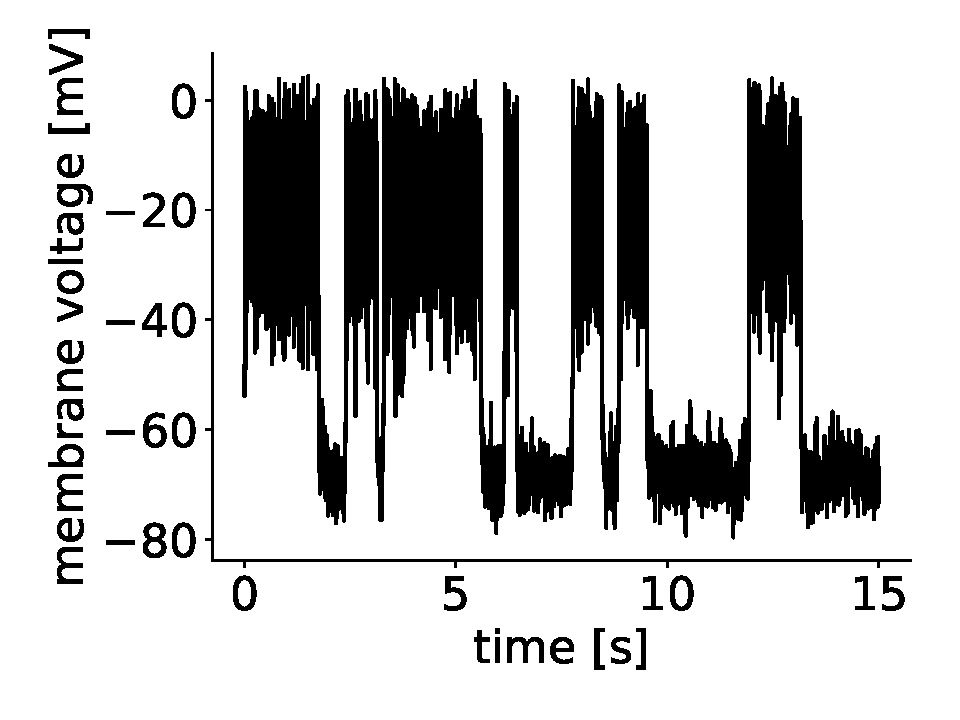
\includegraphics[scale=0.45]{realstatevar14vsh2noleg.pdf}}	\subfigure[]{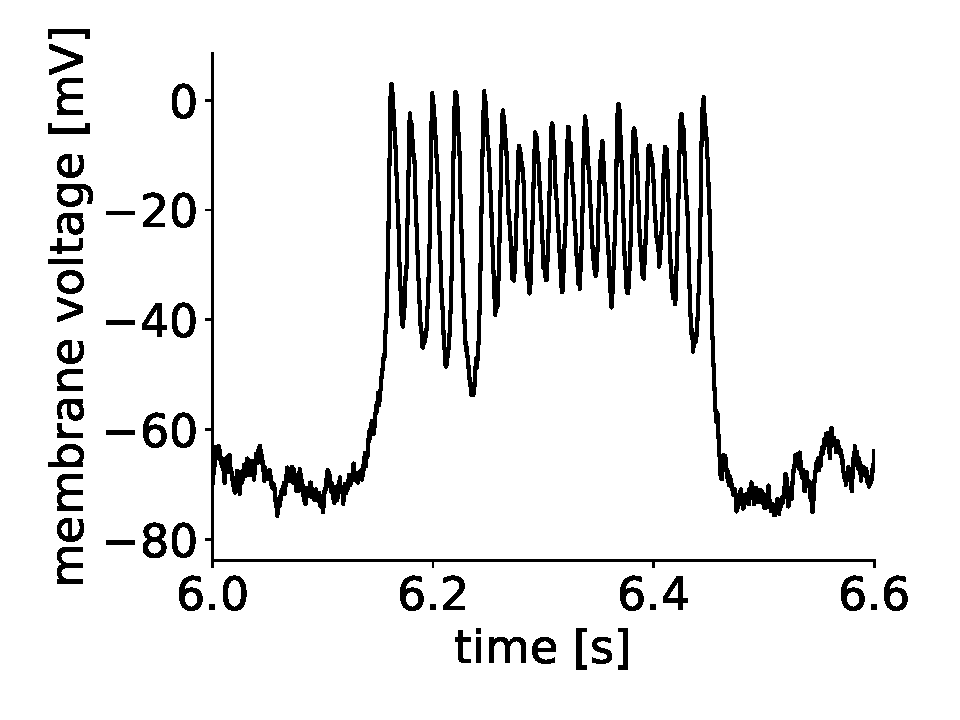
\includegraphics[scale=0.45]{realstatevar14v2noleg.pdf}} 
	\caption{Example of bistable membrane voltage under the influence of noise, obtained from simulations of the $I_{Na,p}+I_K$ model with saddle-node bifurcation with the parameters from section \ref{inapikwsn} and $D=1$. The amplification in (b) illustrates the different qualitative behaviors in both regimes.}
	\label{bistablevolt} 
\end{figure}

A similar bistability has been observed for Brownian Particles in a tilted periodic potential, obeying the following equation of motion\cite{bpp}: 
\begin{equation*}
\dot{v}=-\gamma v-U'(x)+\sqrt{2\gamma kT}\xi(t)
\end{equation*}
with the potential $U(x)=-Fx-d\cos(x)$. $\gamma$ is the friction coefficient, $kT$ the thermal energy which corresponds to the noise intensity and the bias force $F$ determines the tilt of the potential.
 

\begin{figure}[H]
	\subfigure[]{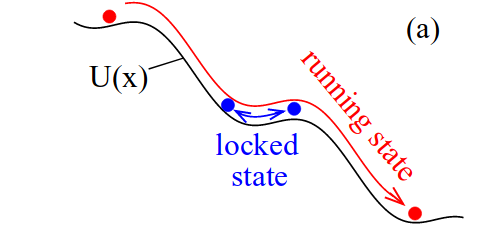
\includegraphics[width=0.5\textwidth]{veldynupper.png}} 
	\subfigure[]{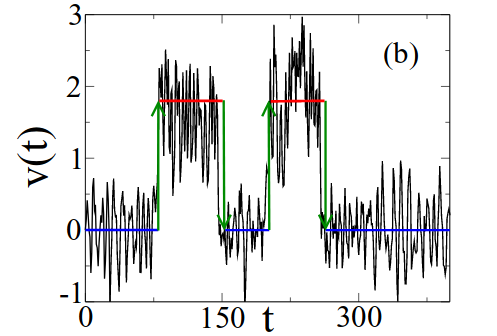
\includegraphics[width=0.5\textwidth]{veldynlower.png}} 
	\caption{Figure (a) visualizes the two motional states of an underdamped Brownian Particle in a periodic potential, on the right one can see the bistable velocity dynamics. The oscillations in the locked state are noise-induced while they mainly arise from local extrema of the potential in the running state. These images have been taken from\cite{bpp}.}
	\label{veldynintro} 
\end{figure}
Assuming that friction is low and $F$ is chosen such that the tilted potential keeps its minima and maxima, the Brownian particle can be in two different velocity states (figure \ref{veldynintro}). If it performs noise-induced oscillations near a minimum, it is in the so-called \textit{locked state}.
After the Brownian particle has managed to overcome a hill and still has enough energy to pass the adjacent maxima as well, it is said to be in the \textit{running state}.
While making its way down the washboard potential, the Brownian particle switches between these states due to the influence of noise.
In the case of large friction or a strongly tilted potential, however, the particle will barely move or move almost all of the time, respectively. In either configuration, one of the states prevails. When an ensemble of Brownian particles are thrown into the system under these conditions, the majority of particles finds itself in the same state of motion. As a consequence, the particles move roughly as a group with only little spread around the mean velocity. Therefore, the effective diffusion coefficient $D_{eff}$ which quantifies the diffusional spread,
\begin{equation}
D_{eff}=\lim_{t\rightarrow\infty}\frac{\left\langle x^2(t) \right\rangle-\left\langle x(t)\right\rangle ^2}{2t}
\end{equation}
becomes very small. The other extreme case is reached when the parameters are chosen in such a way that both states are equally likely. Then, approximately half of the particles are resting while the others are in the running state, leading to a large $D_{eff}$. The lower the noise intensity, the fewer switchings occur and the higher is the effective diffusion coefficient. This phenomenon can be seen in figure (\ref{anbpsimintro}).

\begin{figure}[H]
	\centering
	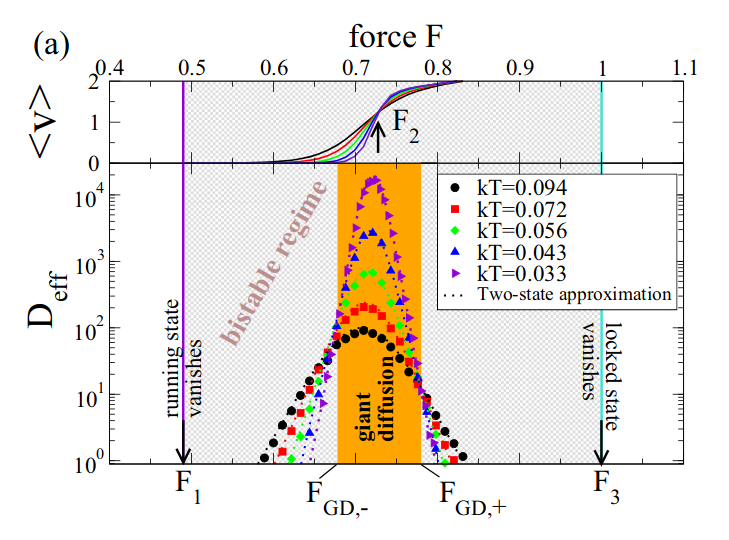
\includegraphics[scale=0.5]{nbpsim1.png}\caption{Simulation of velocity and effective diffusion coefficient for underdamped Brownian Particles in a tilted periodic potential,taken from \cite{bpp}}
	\label{anbpsimintro}
\end{figure}

The upper part of the figure shows the average velocity which naturally increases with the slope of the potential. The noise-dependent bias force where both states are equally likely is here denoted by $F_2$. In the zero-noise limit, bias forces which are smaller than this value lead to a vanishing velocity. As the resting state is more probable than the running state, the particles will eventually end up there. The same argument can be made for $F>F_2$: when the probability is higher to be in the running state than in the resting state, the maximum velocity is achieved. Consequently, all velocity curves make a jump and intersect each other at $F_2$.\\
As explained above, the diffusion coefficient gets maximal when both states are occupied with equal probabilities, which happens at $F_2$. Decreasing the noise results in a higher $D_{eff}$, so it can get arbitrarily large at low noise. This phenomenon is called giant diffusion, which is short for \textit{giant enhancement of (thermal) diffusion} and was first observed around the turn of the millennium for Brownian Particles in a tilted periodic potential\cite{td}\cite{ga}\cite{dit}\cite{gd}. %In general, giant diffusion occurs in systems with two stable velocity states. 
Interestingly, the diffusional growth is not only restricted to this particular bias force, but extends over a finite area between the two intersection points of all curves, $F_{GD,\pm}$. Outside of this region, $D_{eff}$ decreases with the noise intensity. Taking a closer look, one notices that the left intersection lies slightly above the right one. \\
It should be noted that a motion with low diffusion as it occurs outside the region of giant diffusion does not require the disappearance of one of the states, but happens much earlier. Thus, not all particles need to be in the same motional state to accomplish a small diffusion.\\
In order to better understand what happens in the bistable regime, a simplified description can be used. 
In the case of low noise intensity, the transition times between the locked state and the running state will be much shorter than the periods of time that the particle stays in one of the two states. That is why it is practical to describe the behavior of the system with a two-state model. The results of this model are plotted as dotted curves and show good agreement with the data. The transition rates between the states are assumed to obey an Arrhenius law:
\begin{align}\label{arrhlaw}
r_{\pm}=r_{0,\pm}\exp\left(-\frac{\Delta U_{\pm}}{D}\right)
\end{align}
where $r_-$ denotes the transition rate from locked to running state, and $r_+$ the rate for the other transition. $\Delta U_{\pm}$ is the corresponding potential barrier that needs to be traversed and $D$ the noise intensity which previously was $kT$. The effective diffusion coefficient can be calculated from the velocity $v_0$ in the running state and the transition rates\cite{abp}: 
\begin{align}\label{Deff}
D_{\text{eff}}=\frac{v_0^2 r_+r_-}{(r_++r_-)^3}
\end{align}
This formula allows us to find the intersection points of the diffusion coefficients. As the curves for all noise intensities go through these points, they become independent of the noise intensity there. Consequently, they should remain the same also for vanishing noise intensity.
It is
\begin{align*}
D_{\text{eff}}&=\frac{v_0^2r_{0,+}r_{0,-}\exp\left(-\frac{\Delta U_++\Delta U_-}{D}\right)}{\left[r_{0,+}\exp(\frac{-\Delta U_+}{D})+r_{0,-}\exp\left(\frac{-\Delta U_-}{D}\right)\right]^3}\\&=\frac{v_0^2r_{0,+}r_{0,-}}{\left[r_{0,+}\exp\left(-\frac{3\Delta U_+-\Delta U_+-\Delta U_-}{3D}\right)+r_{0,-}\exp\left(-\frac{3\Delta U_--\Delta U_+ -\Delta U_-}{3D}\right)\right]^3}\\&=\frac{v_0^2r_{0,+}r_{0,-}}{\left[r_{0,+}\exp\left(-\frac{2\Delta U_+-\Delta U_-}{3D}\right)+r_{0,-}\exp\left(-\frac{2\Delta U_--\Delta U_+}{3D}\right)\right]^3}
\end{align*}
In the limes $D\rightarrow 0,\Delta U_+\Delta>U_-$ the first term in the denominator vanishes, resulting in:
\begin{align*}
D_{\text{eff}}=\frac{v_0^2r_{0,+}}{r_{0,-}^2}\exp\left(-\frac{\Delta U_+-2\Delta U_-}{D}\right)
\end{align*}
Under the assumption that the prefactors change slowly in comparison to the exponential function, the following condition for the first intersection point arises:
\begin{align}\label{fcrit}
\Delta U_+=2\Delta U_-
\end{align}
Due to symmetry of the problem, the opposing case $D\rightarrow 0,\Delta U_+<U_-$ yields:
\begin{align*}
\Delta U_-=2\Delta U_+
\end{align*}
In both cases, one potential barrier is twice as high as the other one.\\
The verification of this criterion requires knowledge of potential barriers. As there are no actual potential barriers in the system, it is only possible to derive effective barriers from the behavior of the system.
These can be acquired by measuring transition rates at different noise intensities and fitting them with the Arrhenius law from (\ref{arrhlaw}), as it was done in Figure \ref{ratesintro}.
\begin{figure}[H]
	\subfigure[]{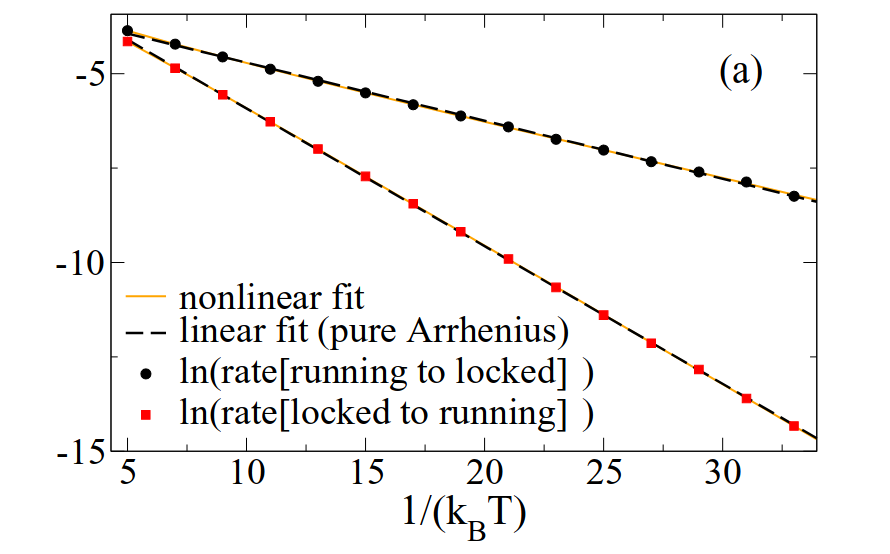
\includegraphics[width=0.5\textwidth]{kramerfit.png}} 
	\subfigure[]{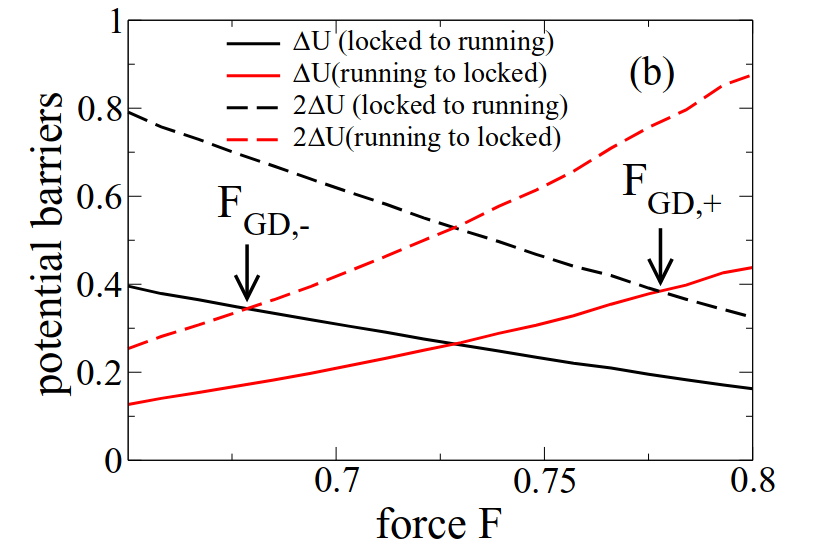
\includegraphics[width=0.5\textwidth]{barrierplot.png}} 
	\caption{The left plot shows the transition rates for a fixed bias force over a range of different noise intensities. Fits were done with both an Arrhenius (equation \ref{arrhlaw}) and a Kramers law that accounts for a temperature-dependence of the prefactor, $r_0\propto T^\alpha$, but yielded similar results for the effective barriers. On the right the effective potential barriers are shown, where the dotted curves are simply twice the solid curves.  The images have been taken from \cite{bpp}.}
	\label{ratesintro} 
\end{figure}
It can be seen that the Arrhenius-like behavior continues over a wide range of noise intensities, allowing to get reliable values for the effective potential barriers. According to the criterion from (\ref{fcrit}), the critical forces are expected to be at 0.68 and 0.78, which roughly corresponds to the actual intersection points.\\
These findings imply that similar systems might show similar behavior, which brings us back to the bistable neurons introduced in the beginning. If every event of a Brownian particle crossing a hill would be interpreted as a spike, the Brownian particle in a tilted potential itself can be seen as a model for bistable neurons. As a consequence, every observable in the here discussed system of Brownian particles has its equivalent in bistable neurons. The position $x$ is proportional to the number of crossed hills, thereby corresponding to the spike count. The velocity denotes the number of hills that are crossed in a certain time interval, which can be related to the firing rate. The neural spiking behavior can be influenced by applying a bias current $I$ which corresponds to the force $F$ determining the tilt of the potential. The noise source is not thermal noise anymore, but channel noise or random input from surrounding neurons. With regard to the results for Brownian particles in a tilted potential, bistable neurons should therefore also display giant diffusion in the form of a strong increase of spike count diffusion over a certain range of bias currents.
\\
In addition to that, it should also be possible to measure transition rates between both states, extract effective potential barriers from these and describe the behavior of a bistable neuron model with the two-state theory. 
\\
As the main purpose of neurons is the transmission of information, the relevance of giant diffusion in neurons can be best understood with regard to signal transmission. The important aspect here is not that the effective diffusion coefficient $D_{eff}$ can get arbitrarily large at low noise but the two critical currents where all curves intersect. Near the critical current, a small change of currents can induce a large increase or decrease of $D_{eff}$. This means that at this point the neuron is very sensitive to variations which can also be caused by an external signal. Thus, it is to be expected that the quality of signal transmission improves strongly near the critical current.
\\
The quality of signal transmission can be quantified by the signal-to-noise ratio SNR which compares the amplitude of the signal to the noise background. The behavior of the SNR in neurons has already been treated analytically under the assumption of some simplifications. If the system is driven by a slow cosine signal with amplitude $\epsilon$ and the noise background is approximated by $D_{eff}$ the signal-to-noise ratio can be computed via\cite{snr}
\begin{align*}
SNR=\frac{\epsilon ^2T}{8}\frac{|\chi(0)|^2}{D_{eff}}
\end{align*}
where $\chi$ denotes the susceptibility and $T$ the total simulation time. This formula confirms our previous conjecture: near the critical current, the spike count diffusion would change by multiple orders of magnitude, leading to a similar, opposite change in the SNR. \\
All in all, bistable neuron models are suggested to exhibit giant diffusion and therefore possess critical currents. When the system is near such a critical point, slight changes in the bias current can cause strong changes in the SNR and possibly a large enhancement of signal transmission. The goal of this thesis is to find out whether giant diffusion exists for neuron models, investigate possible consequences for signal transmission and try to describe the findings with the two-state theory. In order to do that, three different systems are examined in this thesis: both the $I_{Na,p}+I_K$ model with saddle-node bifurcation off invariant cycle and with subcritical Andronov-Hopf bifurcation\cite{izi} as well as a two-dimensional simplification of the Hodgkin-Huxley model that was proposed by Rinzel\cite{rinzel}. In section \ref{modmet}, the general behavior of these models is discussed, including phase plane analysis and the influence of initial conditions and different bias currents. The count statistics of all models are presented in section \ref{countstat}. In section \ref{tranrates}, the findings are compared to the two-state theory based on transition rates between the states. Finally, section \ref{con} shows the influence of a periodic signal on the systems and once again compares the measurements with the two-state theory.
\newpage
\section{Models and Methods}\label{modmet}
\subsection{The $I_{Na,p}+I_K$ model with saddle-node bifurcation}\label{inapikwsn}
The main focus of this thesis lies on the study of the $I_{Na,p}+I_K$-model, the persistent sodium plus potassium model with additive noise:
\begin{align}\label{Veq}
C\dot{V} &= I - g_L(V-E_L) - g_{Na}m_{\infty}(V)(V-E_{Na}) - g_Kn(V-E_K)+\sqrt{2D}\xi(t)\\\label{neq}
\dot{n} &= (n_{\infty}(V)-n)/\tau(V)
\end{align}
Here, $V$ denotes the membrane voltage, $C$ is the capacitance, $I$ is the bias current, $g_i$ are conductances and $E_i$ the Nernst equilibrium potentials. Noise with intensity $D$ was added to make the system burst. Lastly, $m_{\infty}$ is the activation variable of the instantaneous $Na^+$ current, while $n$ governs the variation of the slower $K^+$ current. The steady-state activation functions are approximated by a sigmoid function:
\begin{align*}
f_{\infty}(V) = \frac{1}{1+\exp\{(V_{1/2}-V)/k\}}
\end{align*}
At $V_{1/2}$, the activation function has the value 1/2, and $k$ is the slope factor determining the steepness around $V_{1/2}$ - a smaller value of $k$ leads to a more abrupt change of $f_{\infty}$. This approximation was suggested by Izhikevich \cite{izi}.\\
The fastest neural oscillations in the human brain are gamma waves with frequencies in the range between 25 and 100 Hz\cite{gamma}\cite{gamma2}. Similar values can also be found in different papers about bursting neurons\cite{burstneu}\cite{burstneu2}. Therefore, the parameters were chosen such that the frequency in the bursting state was about 70 Hz.
The exact values used in the simulations were:\\\\
$C=1$ , $g_L=0.3$ , $E_L=-80$ , $g_{Na}=1$ , $E_{Na}=60$ , $g_K=0.4$ , $E_K=-90$.
\begin{align*}
\intertext{Instantaneous $Na^+$ current:} k_m&=14 , V_{1/2,m}=-18. 
\\
\intertext{$K^+$ current:} k_n&=5 , V_{1/2,n}=-25 , \tau(V)=\text{const}=3.
\end{align*}
%\subsubsection{Phase plane analysis}
\subsubsection{System without noise}\label{mod1won}
The qualitative behavior of the neural model can be best understood by first considering the noiseless system.
For a system that depends on the evolution of two state variables, in this case $V$ and $n$, some qualitative and quantitative analysis can be carried out in the phase plane. A neat way to obtain information about an unknown system is to calculate its nullclines. The nullclines are curves in the phase plane where one of the state variables remains constant. Thus, the $V$-nullcline is defined by the condition $\dot{V}=0$ and the $n$-nullcline follows from $\dot{n}=0$. By crossing one of the nullclines, the system changes its direction of motion with respect to the corresponding variable. As a consequence, each nullcline separates the phase space into two regions where one of the variables evolves in opposite directions. Taken together, the nullclines define four different regions of directions: one region each where both variables decrease or increase and two regions where one variable increases and the other decreases. Depending on the specific shape of the nullclines, these regions do not necessarily have to be coherent.\\
The $V$-nullcline can be obtained by setting the left side of equation (\ref{Veq}) to zero. In the $V$-$n$-plane, it can then be described by the function
\begin{align}
n(V)=\frac{I - g_L(V-E_L) - g_{Na}m_{\infty}(V)(V-E_{Na})}{g_K(V-E_K)}
\end{align} 
The $n$-nullcline is just
\begin{align}
n(V)=n_\infty(V)
\end{align}
The nullclines of the $I_{Na,p}+I_K$-model are shown in figure \ref{realnc}.\\
A second aspect of the nullclines are their intersection points. As both state variables remain constant when the nullclines intersect, these points are equilibrium points.\\
In general, there are three different types of equilibria: nodes, saddles and foci. These may be stable or unstable. Any trajectory in the phase space starting close enough to a stable equilibrium stays near it for all times. In contrast to that, an equilibrium is unstable, if at least one trajectory that starts arbitrarily close to it diverges from the equilibrium.
If they are in the vicinity of a node, all trajectories either converge to or diverge from it. A saddle can be approached along one of the nullclines but is repelling along the other nullcline. Therefore, most trajectories first approach the equilibrium point and then diverge from it. Trajectories that start near a focus rotate around the equilibrium point and thereby get closer to or farther away from it. 
%\subsubsection{Jacobian matrix of the system}
The equilibrium points can be characterized by studying the Jacobian matrix of the system at these points. A two-dimensional system can be written in the form
\begin{align}
\dot{x}=f(x,y)\\
\dot{y}=g(x,y)
\end{align}
Utilizing the fact that the functions $f$ and $g$ can be linearized near the equilibrium, which means they can be approximated by the first term of their Taylor expansion, one finds a linear system at the equilibrium $(x_0,y_0)$:
\begin{align}				
\left(\begin{matrix}\dot{u}\\\dot{w}
\end{matrix}\right)
=\left(\begin{matrix}a\quad b\\
c\quad d\end{matrix}\right)\left(\begin{matrix}u\\w\end{matrix}\right)=L\left(\begin{matrix}u\\w\end{matrix}\right)
\end{align}
where $u=x-x_0$, $w=y-y_0$, $L$ is the Jacobian matrix at equilibrium and the coefficients are the partial derivatives
\begin{align}
a=\frac{\partial f}{\partial x}(x_0,y_0),\qquad b=\frac{\partial f}{\partial y}(x_0,y_0) \\
c=\frac{\partial g}{\partial x}(x_0,y_0),\qquad d=\frac{\partial g}{\partial y}(x_0,y_0)
\end{align} 
Having determined the eigenvalues $\lambda_\pm$ and eigenvectors $ \boldsymbol{v_\pm}$ of $L$, a solution for the linear system can be constructed:
\begin{align}
\left(\begin{matrix}u(t)\\w(t)
\end{matrix}\right)=c_+\boldsymbol{v_+}\exp(\lambda_+t)+c_-\boldsymbol{v_-}\exp(\lambda_-t)
\end{align}
At this point, the connection between the Jacobian matrix and the different types of equilibria becomes clear. If both eigenvalues are real and have the same sign, both terms of the solution either grow or decay exponentially, meaning that the equilibrium is a node. If they are real with opposite signs, the equilibrium point is a saddle. Finally, if the eigenvalues are complex-conjugate, the solution oscillates, which makes the equilibrium a focus\cite{izi}.\\
When no bias current is applied (that is, I=0), the system features three equilibrium points:
\begin{figure}[H]
	\centering
	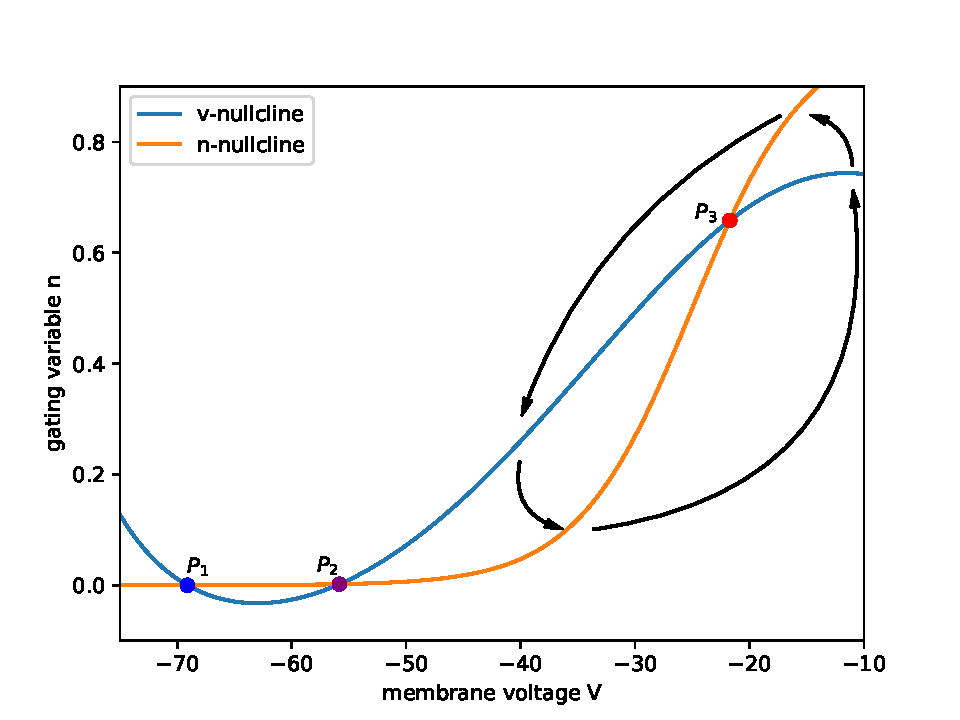
\includegraphics[scale=0.95]{inapikrealncwnp.pdf}\caption{Nullclines of the $I_{Na,p}+I_K$-model with $I=0$. The arrows indicate the direction of motion in the different regions.}
	\label{realnc}
\end{figure}
Carrying out the phase plane analysis, one finds:
\begin{align*}
\lambda_+(P_1)&\approx-0.1 & \lambda_-(P_1)&\approx-0.3\\
\lambda_+(P_2)&\approx 0.1& \lambda_-(P_2)&\approx -0.3\\
\lambda_+(P_3)&\approx 0.05 + 0.5i& \lambda_-(P_3)&\approx 0.05 - 0.5i
\end{align*}
This means that $P_1$ is a stable node, $P_2$ is a saddle point and $P_3$ is an unstable focus. Thus, in the bursting state, the phase vector will rotate around $P_3$, approach $P_2$ in $n$ - direction and then go away from $P_2$ in $V$ - direction in order to do another rotation around $P_3$.\\
However, this applies only to the case of small bias currents. When $I\approx 0.36$, the saddle and the node fall together and the system undergoes a saddle-node bifurcation off invariant circle. In this case, the resting state vanishes and the neuron is in a state of tonic spiking.
\\
Provided that we are in the bistable regime, a system with arbitrary initial conditions will either go to the resting or the spiking state and will not change its behavior anymore after a short period of equilibration, as can be seen in figure \ref{subfig}. 
\begin{figure}[H]
	\subfigure[]{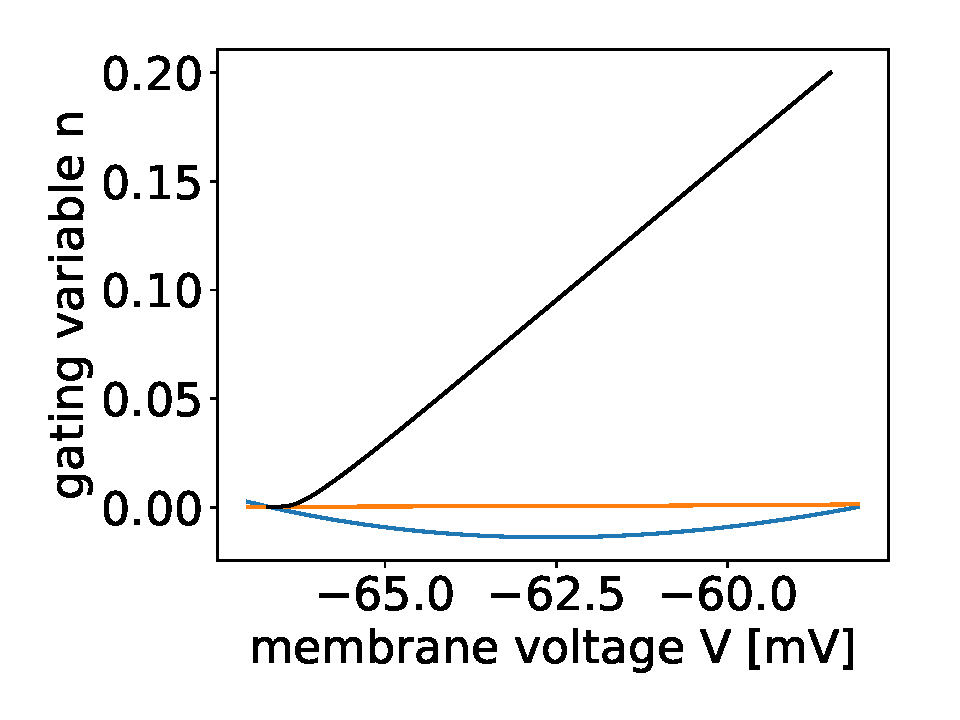
\includegraphics[scale=0.45]{inapreali20nbfontblack.pdf}} 
	\subfigure[]{	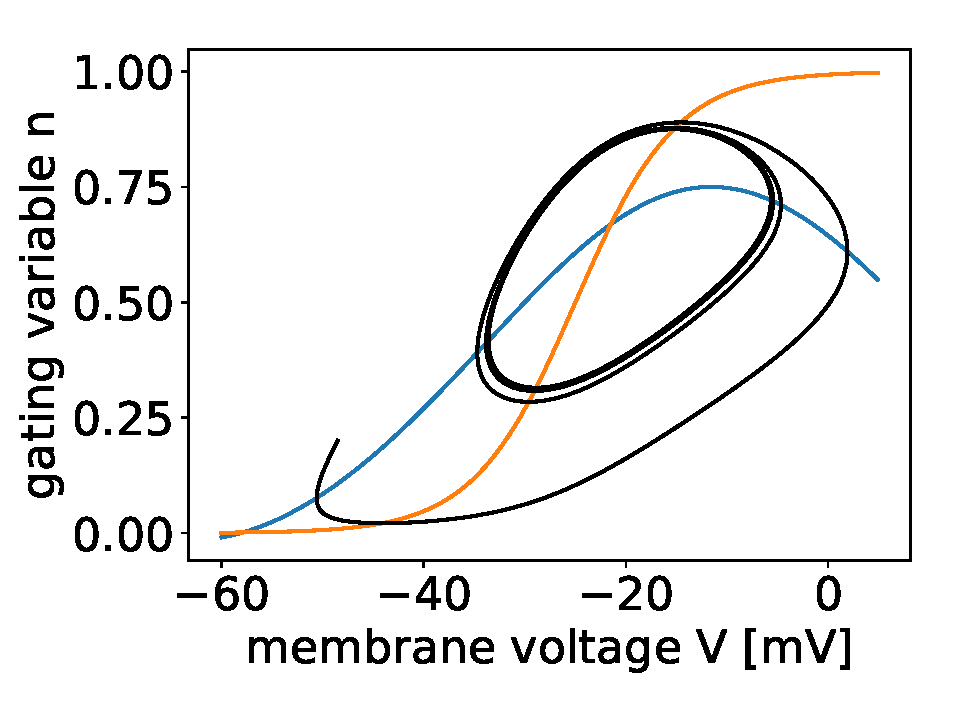
\includegraphics[scale=0.45]{inapreali20fontblack.pdf}}\\	\subfigure[]{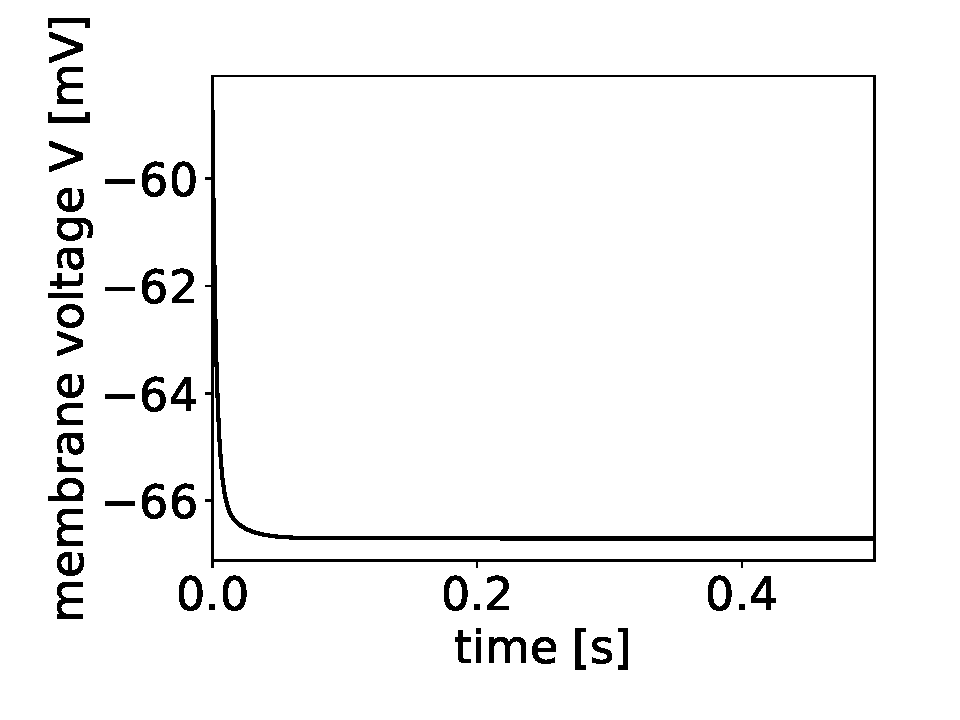
\includegraphics[scale=0.45]{inapreali20nbvfontblack.pdf}} 
	\subfigure[]{	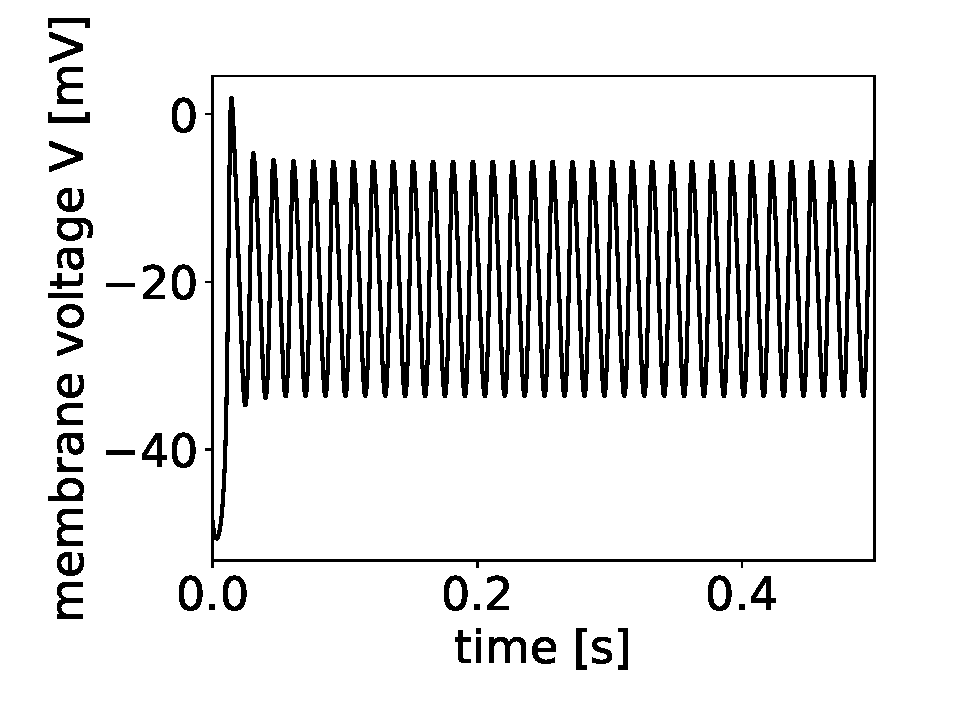
\includegraphics[scale=0.45]{inapreali20vfontblack.pdf}}
	\caption{Evolution of the phase vector (first row) and the membrane voltage over time (second row).
		The left side shows the evolution of the system with resting initial conditions (ICs), and on the right one can see the behavior under spiking ICs.}
	\label{subfig} 
\end{figure}
Analytically, it is hardly possible to determine whether a specific starting point ($V_0$,$n_0$) leads to repetitive spiking or no spiking at all. The only thing one can say for sure is that the line that separates both domains will go through the saddle point that was found in the phase plane analysis. Assuming that the gating variable does not change, any trajectory starting at higher voltages will lead to spiking while all trajectories at lower voltage converge to the stable node. A numerical investigation of the model without noise confirms our conjecture (figure \ref{twodom}).
\begin{figure}[H]
	\hspace*{-0.5cm}
	\subfigure[]{	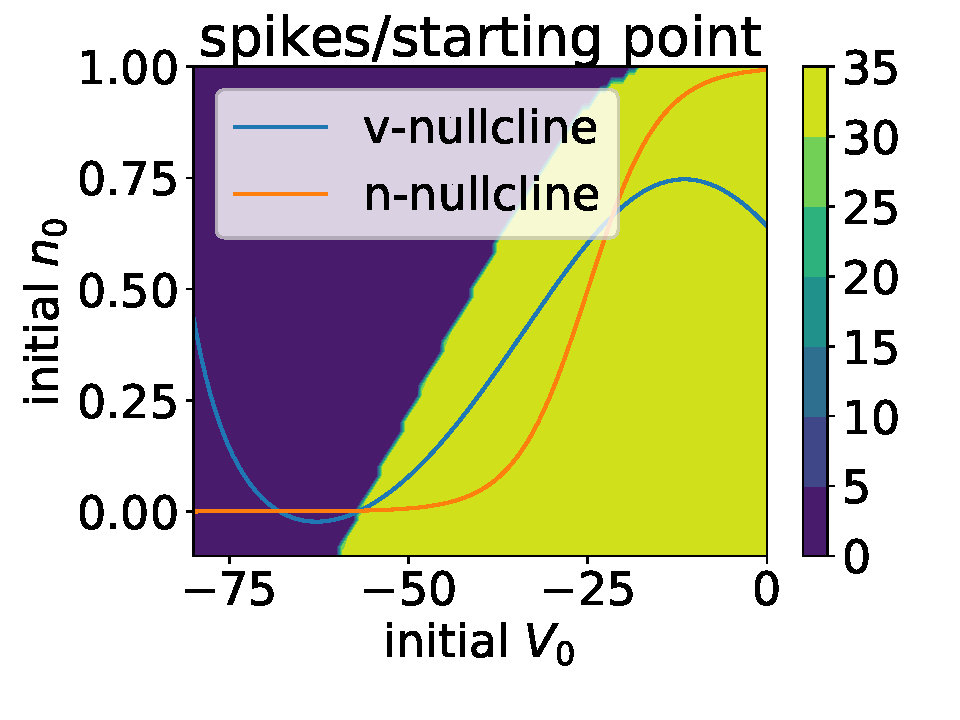
\includegraphics[scale=0.45]{contourtime01wn2.pdf}}
	\subfigure[]{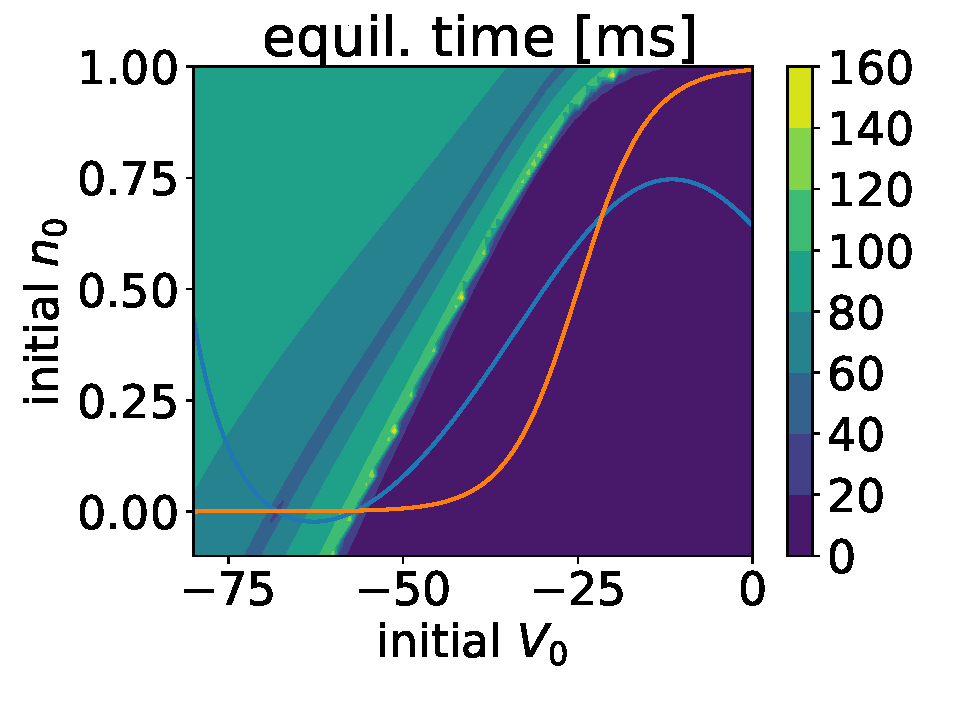
\includegraphics[scale=0.45]{contoureqtime01wn3.pdf}}
	
	\caption{Phase plane of the neuron model with $I=0.1$ and no noise. Each point represents a specific combination of starting parameters. The left plot shows the number of spikes over a short period of time and for the right figure, the equilibration times for both states were measured. Irregularities arise from the finite resolution of the $V_0$-$n_0$-lattice.}
	\label{twodom}
\end{figure}		
There are two distinct regions which can be separated by a monotonically increasing curve that passes through the saddle point. In figure \ref{twodom}b one can see a small intermediate area of large equilibration times. If the system parameters lie in the vicinity of this transition area, a small perturbation suffices to bring the system into either state. Remarkably, most of this area is made up by starting points leading to the stable equilibrium while only a small streak consists of spiking initial conditions. Consequently, the spiking state is reached much faster than the resting state.
\subsubsection{System with noise}
When noise is brought into the system, the findings for the noiseless system still apply to a great extent. Starting in one of the two domains, the system will most likely first converge to the corresponding state, and the time it takes for that will be about the same as before. However, the system will not stay in this state forever, but perform noise-driven transitions between the states. Thus, it will not be possible anymore to assign an end state to each set of initial conditions. Both transition rates, meaning from running to resting and in the opposite direction, will grow when the noise intensity $D$ increases. \\
In addition to that, depending on the overall configuration, the system is usually biased towards one of the states. It is to be expected that at low bias current $I$, the resting state dominates and the running state is favored at high $I$. Considering the simulations (figure \ref{currentnoise}), this turns out to be a valid hypothesis: At $I=-0.1$, the neuron almost immediately returns to the resting state once it has gotten into the running state. At a slightly higher bias current of $I=0$, the periods of stay in both states are almost equal, and at $I=0.15$, the system is in the running state for the majority of time. The firing frequency in the running state is at about 70 Hz.
\begin{figure}[H]
	\subfigure[]{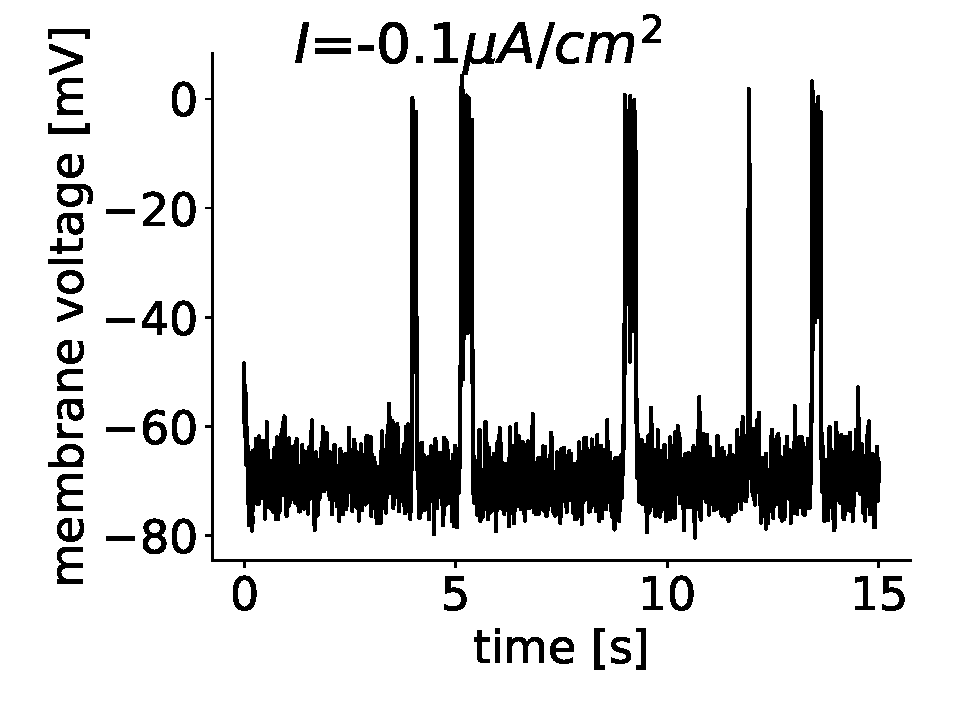
\includegraphics[scale=0.4]{realstatevar1252.pdf}} 
	\subfigure[]{	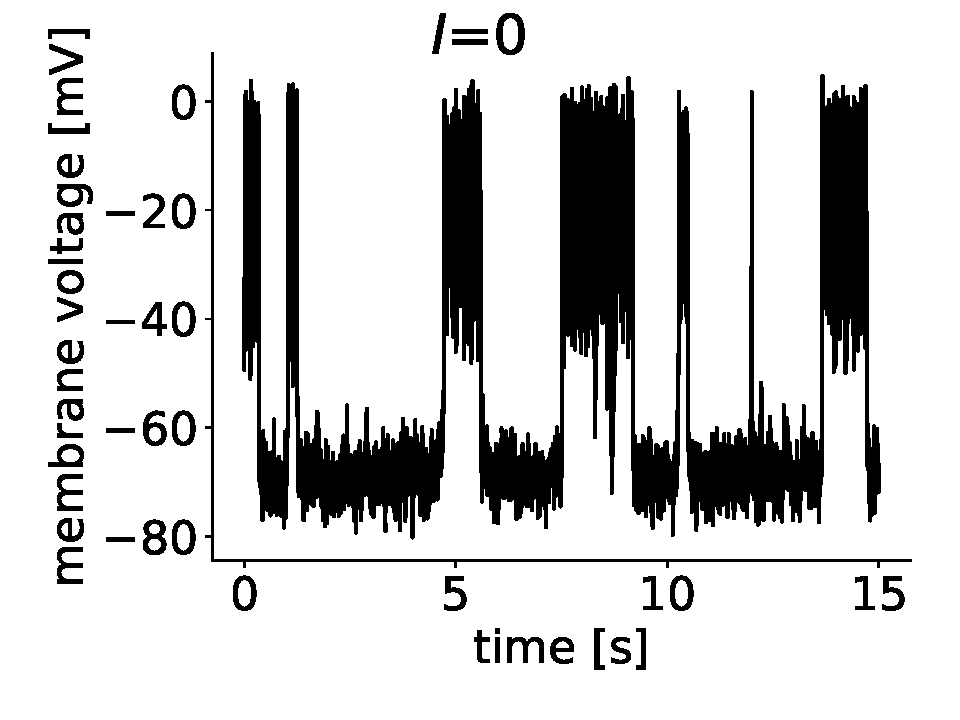
\includegraphics[scale=0.4]{realstatevar1352.pdf}}\\	\subfigure[]{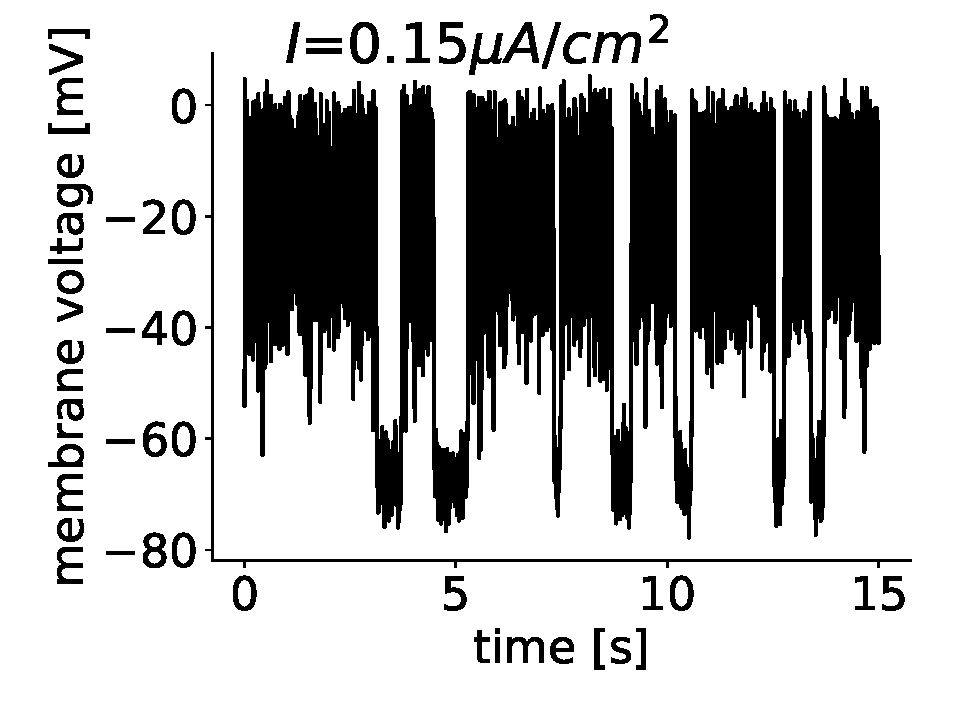
\includegraphics[scale=0.4]{realstatevar152.pdf}} 
	\subfigure[]{	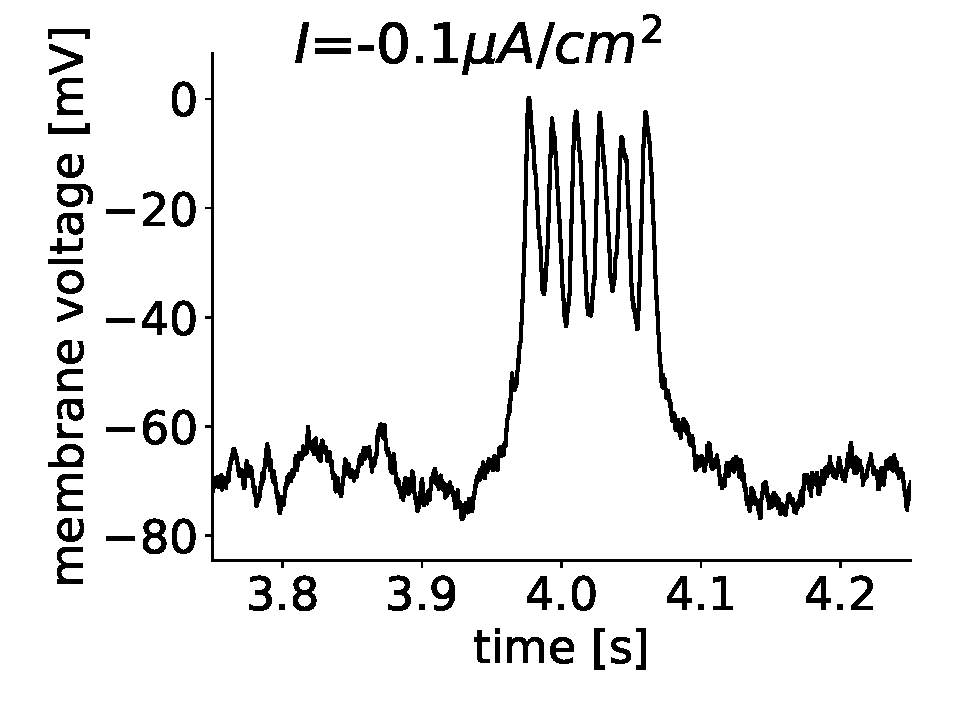
\includegraphics[scale=0.4]{realstatevar125vsh2.pdf}}
	\caption{(a)-(c): Behavior of the membrane voltage for constant noise $D=1$ and changing bias currents $I$. In figure (d), a segment with a higher time resolution is shown in order to better illustrate the evolution of the voltage variable.}
	\label{currentnoise} 
\end{figure}
The figure with a higher time resolution illustrates the influence of noise on a system that is mainly composed of two states. Even though the neuron fires at a regular frequency in the firing state, the peak heights vary by up to 10 mV. Actually, the membrane voltage in the resting state is not really at rest but mostly fluctuates in a range of 20 mV, and also the transition between the states happens quite irregularly.
\begin{figure}[H]
\hspace*{-0.5cm}
\subfigure[]{	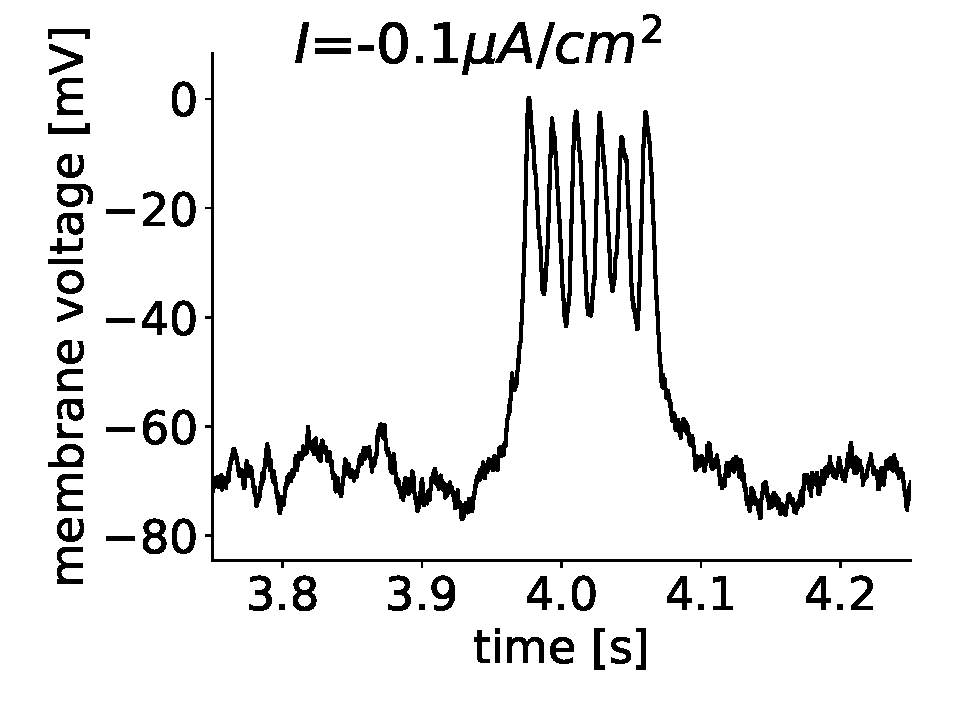
\includegraphics[scale=0.45]{realstatevar125vsh2.pdf}}
\subfigure[]{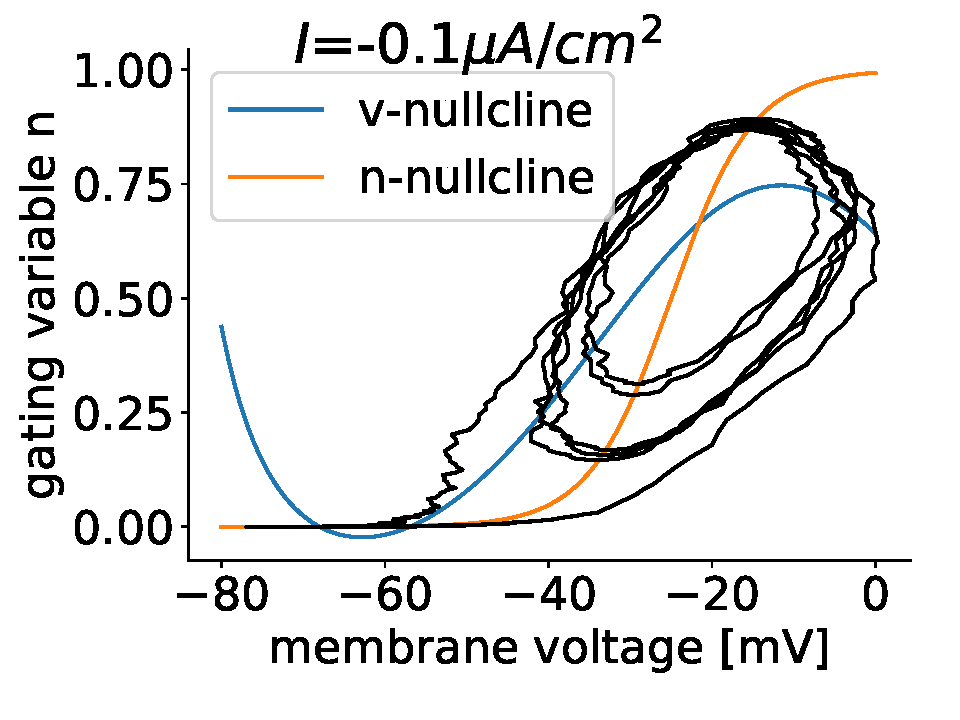
\includegraphics[scale=0.45]{realstatep125vshbig.pdf}}

\caption{Evolution of the membrane voltage over time (left) and the corresponding phase space.}
\label{ppcompneur}
\end{figure}
This can be even better understood in the phase space (figure \ref{ppcompneur}).
One can see that all spikes correspond to rotations around the unstable equilibrium point. The first spike of the burst has a higher amplitude than the rest, corresponding to a larger radius of the limit cycle in the phase space. After that, there are three spikes of equal height (and phase space radius), followed by an even smaller spike. The last spike has a similar phase space trajectory until it reaches the V-nullcline, where it deviates towards a higher voltage, before it finally falls back to the resting state, giving it a larger amplitude again. This is somewhat counter-intuitive, as one would think that the system is more likely to go back to the resting state from a spike with lower amplitude. Apparently, cycles with small radii are more stable than those with large radii. Thus, in order to go into the resting state, the system needs to depart to the outside of the cycle, which may also result in a higher amplitude of the last spike in a burst.\\
Interestingly, the resting neuron only seems to experiences changes in $V$, but not in $n$. This can be easily understood by taking another look at equation \ref{neq}. The variable directly influenced by noise is $V$. The changes are then carried on to $n$ via $n_\infty(V)$. The equilibrium point is now so far on the left end of the n-nullcline, that even variations by tens of mV basically do not induce any change in $n_\infty(V)$. Therefore, we only see fluctuations in the membrane voltage $V$ here. Of course the gating variable is still subject to perturbations, these just happen on a much smaller scale.
%\subsubsection{System with periodic signal}
\subsection{$I_{Na,p}+I_K$ model with subcritical Andronov-Hopf bifurcation}
If we observe giant diffusion in our simulations, it most certainly will not be restricted to only one neuron model. Therefore, it is of particular interest to possibly confirm this behavior also for other bistable two-dimensional neuron models. Finding out in which cases giant diffusion occurs may help to determine conditions that need to be fulfilled and eventually lead to experiments supporting these findings. Therefore two more models will be discussed in the following.
The first one is again the $I_{Na,p}+I_K$ model.
This model is very versatile and displays a wide variety of qualitative and quantitative behavior upon parametric adjustments. Thus, its features can be tweaked such that the system undergoes an Andronov-Hopf bifurcation when the bias current passes a certain value. As presented in section 3, the system is decribed by equations \ref{Veq} and \ref{neq}. The parameters now were the following:\\\\
$C=1$ , $g_L=1$ , $E_L=-78$ , $g_{Na}=4$ , $E_{Na}=60$ , $g_K=4$ , $E_K=-90$.
\begin{align*}
\intertext{Instantaneous $Na^+$ current:} k_m&=7 , V_{1/2,m}=-30. 
\\
\intertext{$K^+$ current:} k_n&=5 , V_{1/2,n}=-45 , \tau(V)=\text{const}=1.
\end{align*}
\subsubsection{System without noise}\label{anhopfwon}
Due to the parameter adjustments one obtains a slightly different phase space image:
\begin{figure}[H]
	\centering
	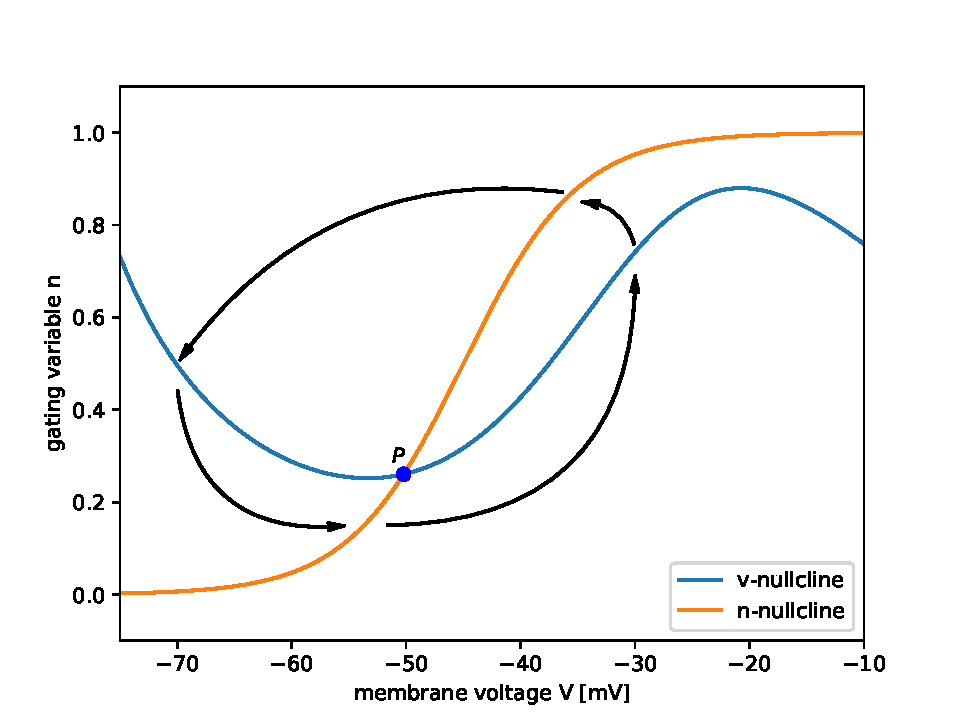
\includegraphics[scale=0.95]{inapikanhopfnc.pdf}\caption{Nullclines of the adjusted $I_{Na,p}+I_K$-model with $I=46$. The arrows indicate the direction of motion in the different regions.}
	\label{anhopfnc}
\end{figure}
The new nullclines yield only one equilibrum point. Computing the Jacobian matrix, following eigenvalues arise for this point:
\begin{align*}
\lambda_+(P)&\approx -0.05 + 2.3i& \lambda_-(P)&\approx -0.05 - 2.3i
\end{align*}
Complex eigenvalues with negative real parts indicate a stable focus. As before, the system performs large oscillations around the focus when it is in the running state. When it is near the equilibrium, it converges fast to it, with the exception that it doesn't approach it directly but oscillates around it with decreasing radius.
In contrast to the previous case, the system now not only consists of stable limit cycle and equilibrium but also an unstable limit cycle in between the two stable configurations. Considering that the system is under the influence of noise, it will not spend much time in the unstable state and quickly collapse into a stable configuration.\\
Upon increase of the bias current, the unstable limit cycle shrinks. At $I\approx 48.9$, it falls together with the stable equilibrium and makes it lose stability. This transition is called a subcritical Andronov-Hopf bifurcation.\\
While in the first model the states were characterized by oscillations around different equilibria, the state vector now only rotates around one equilibrium point. The current state can thereby be identified via the radius of the oscillations. Resting initial conditions result in a small radius and asymptotic convergence to the focus and spiking initial conditions just lead to regular firing with a larger radius, as can be seen in figure \ref{subfigah}. Compared to the first model, the spiking limit cycle is not an ellipse anymore but displays some irregularities.
\begin{figure}[H]
	\subfigure[]{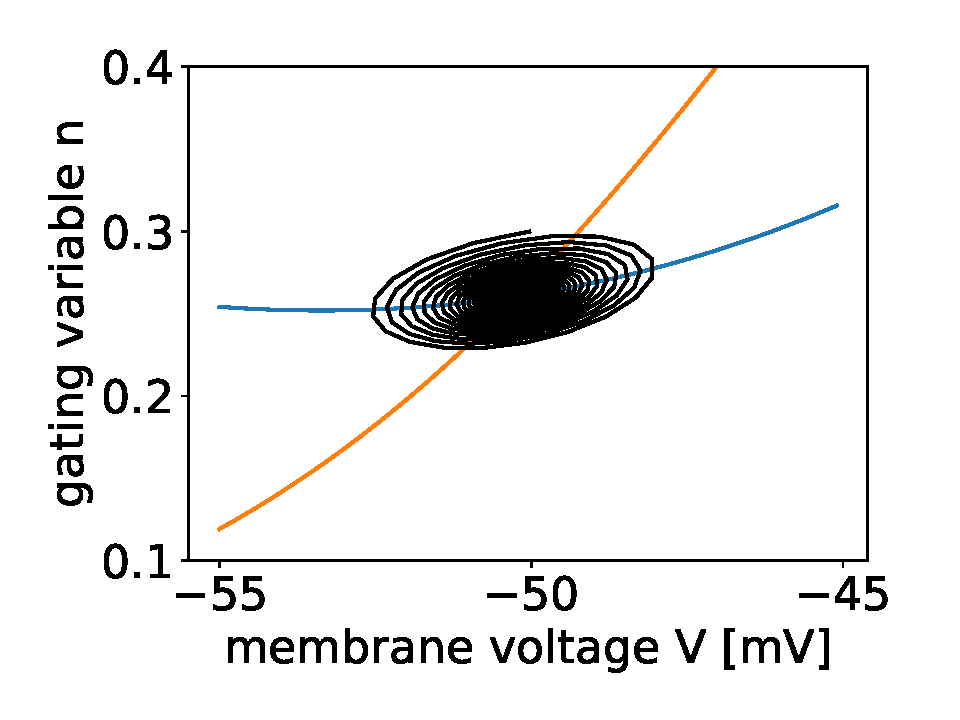
\includegraphics[scale=0.45]{inaprealanhopfnbblack.pdf}} 
	\subfigure[]{	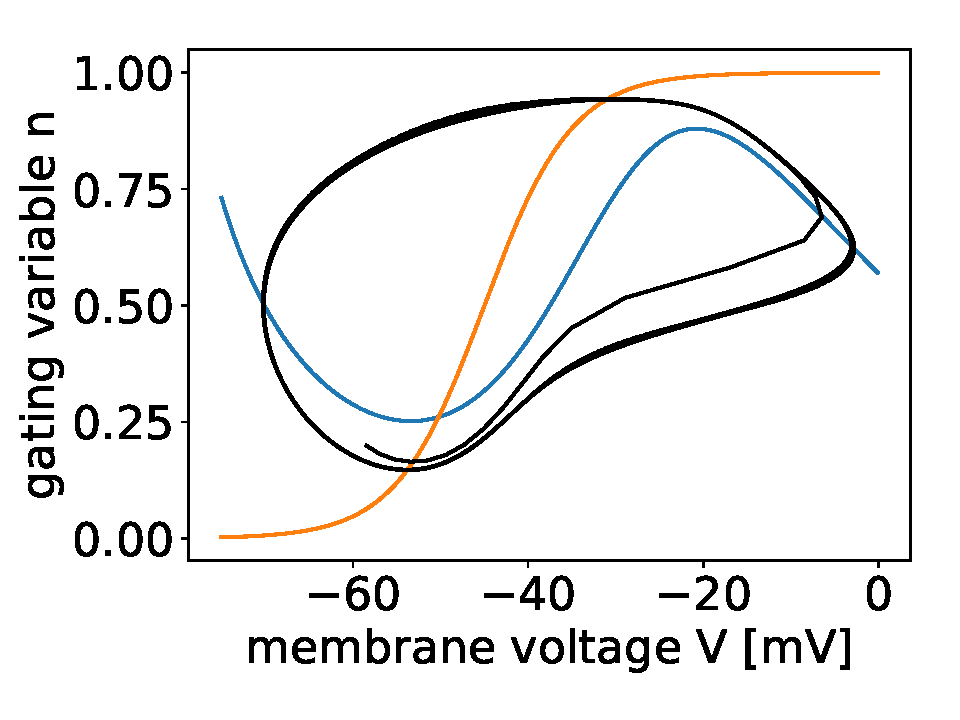
\includegraphics[scale=0.45]{inaprealanhopfblack.pdf}}\\	\subfigure[]{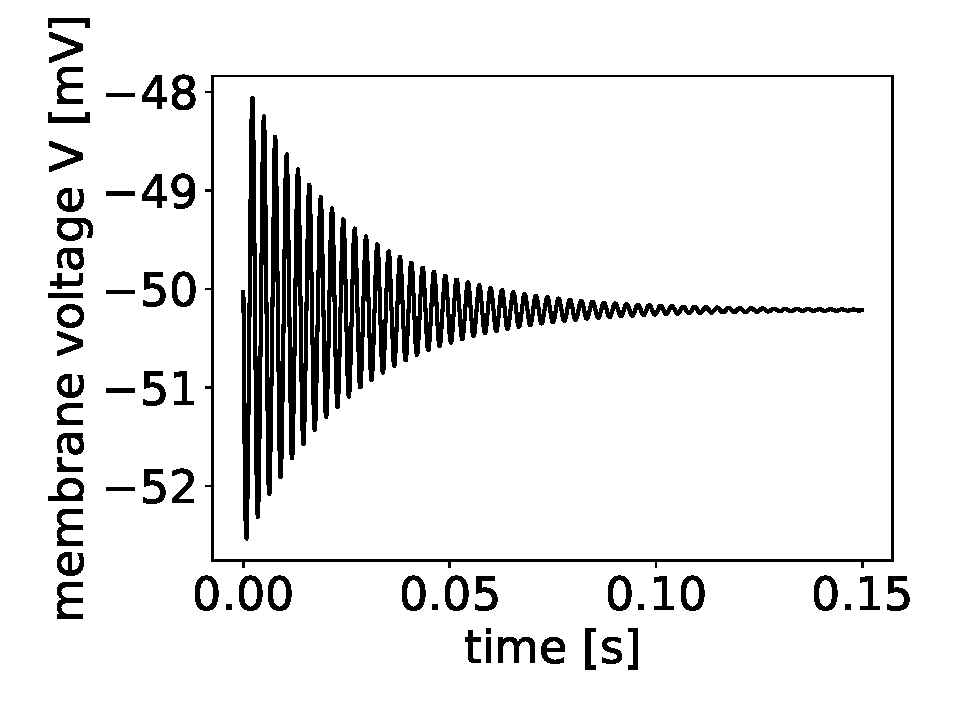
\includegraphics[scale=0.45]{inaprealanhopfnbvtblack.pdf}} 
	\subfigure[]{	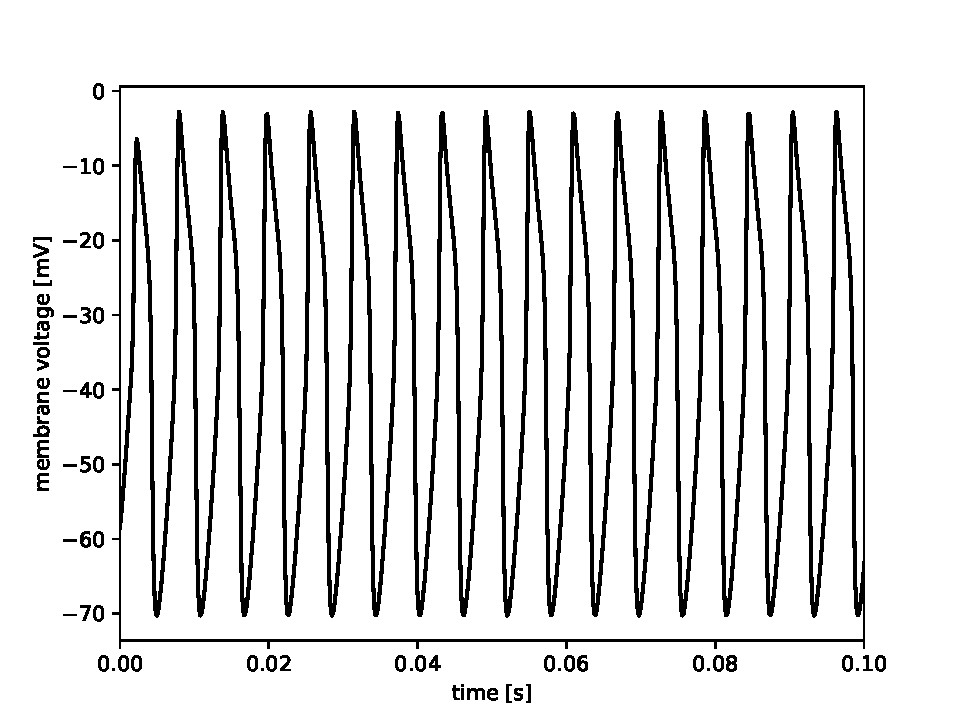
\includegraphics[scale=0.45]{inaprealanhopfvtblack.pdf}}
	\caption{Evolution of the phase vector (first row) and the membrane voltage over time (second row). The left side shows the evolution of the system with resting ICs, and on the right one can see the behavior under spiking ICs.}
	\label{subfigah} 
\end{figure}

\begin{figure}[H]
	\hspace*{-0.5cm}
	\subfigure[]{	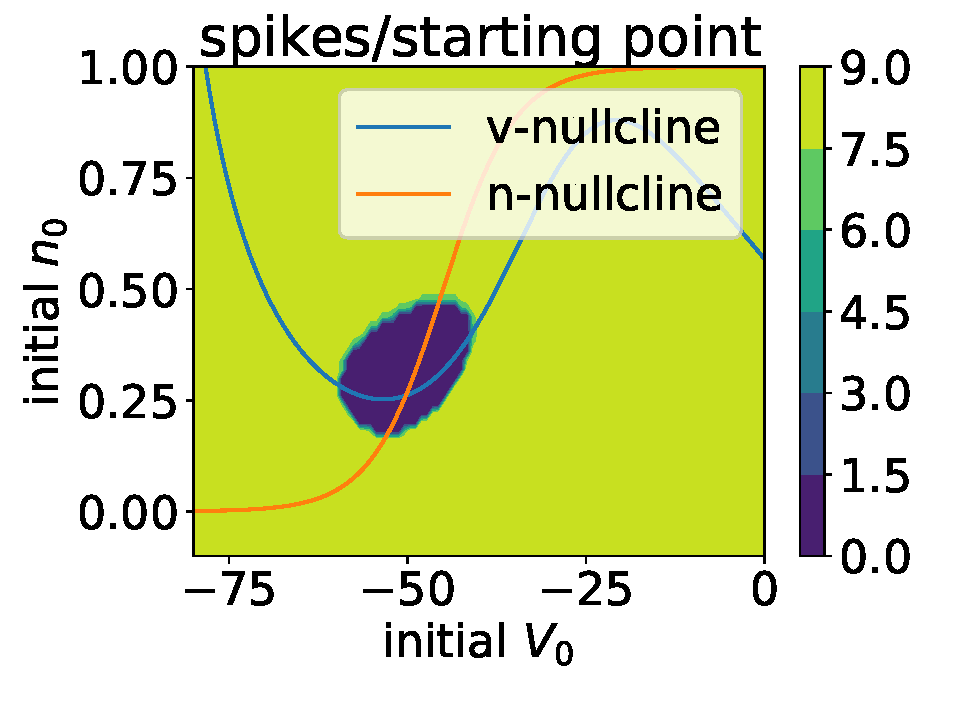
\includegraphics[scale=0.45]{contouranhopfa2sh.pdf}}
	\subfigure[]{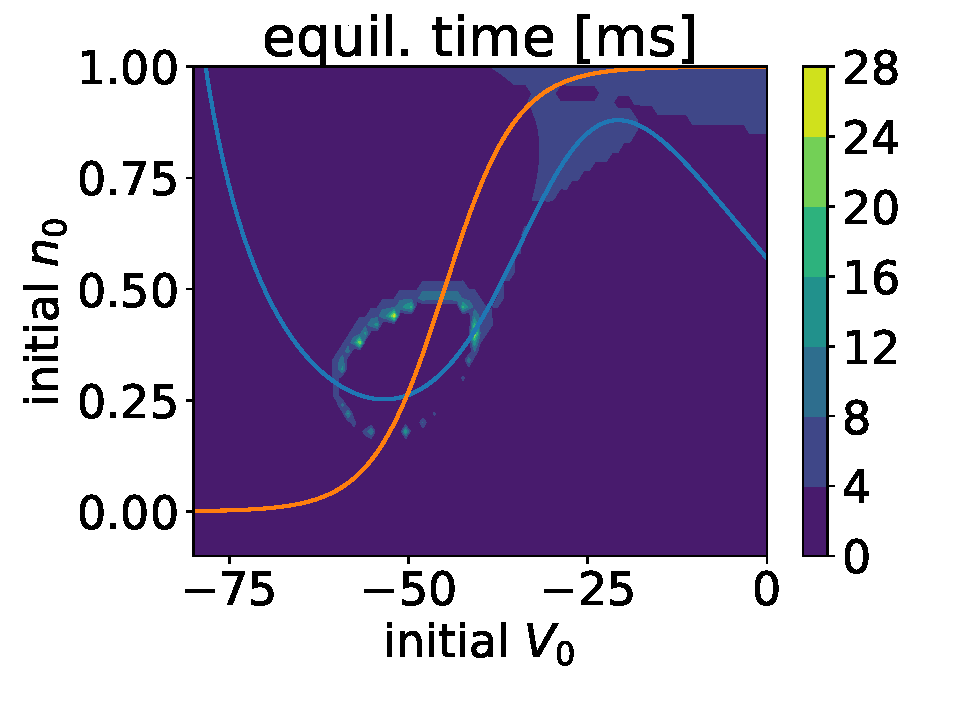
\includegraphics[scale=0.45]{contouranhopfa2time.pdf}}
	
	\caption{Phase plane of the neuron model with $I=46$ and no noise. Each point represents a specific combination of starting parameters. The left plot shows the number of spikes over a short period of time and for the right figure, the equilibration times for both states were measured. In both images one can see the shape of the unstable limit cycle that separates both domains. Irregularities arise from the finite resolution of the $V_0$-$n_0$-lattice.}
	\label{twodom2}
\end{figure}
In order to be able to distinguish between spiking and resting initial conditions, one may simulate the system at different starting points and see how it evolves, as has been done in section \ref{mod1won}.
The area of resting initial conditions is completely enclosed by the spiking regime. Near the border, the system takes longer to equilibrate. This is due to the unstable limit cycle which separates both regimes. By crossing this ellipse from within or from the outside, the system goes over into the firing or resting state, respectively. The course of the unstable limit cycle can be seen in figure \ref{unstable}. These figures were obtained by simulating the neuron model backward in time. That way, unstable regions are turned into stable ones and vice versa. 
\begin{figure}[H]
	\subfigure[]{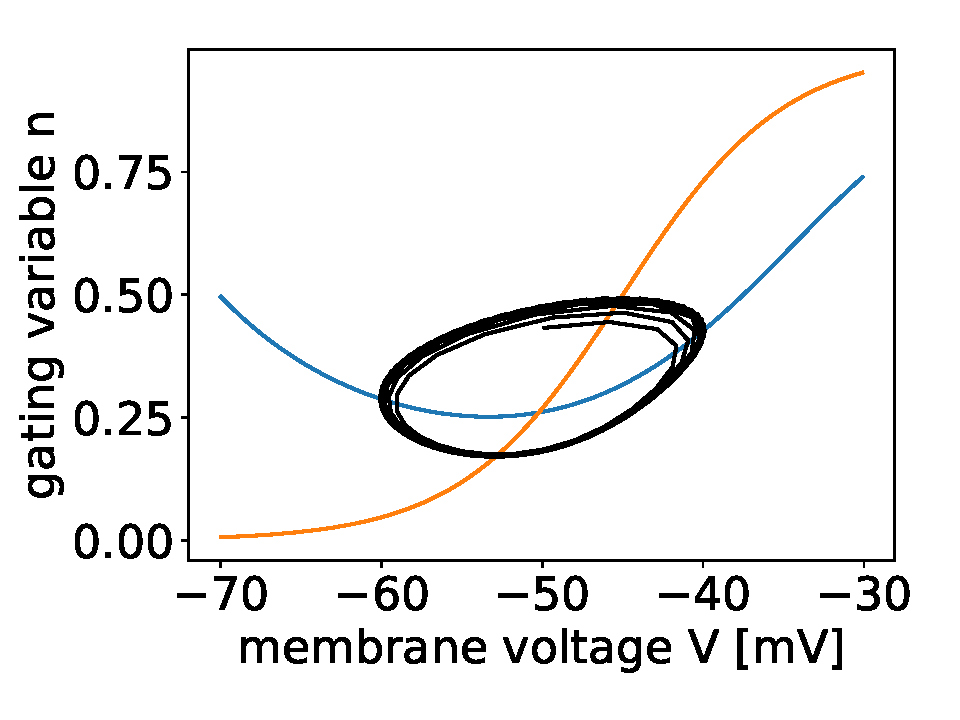
\includegraphics[scale=0.45]{inaprealanhopfunstablewn2black.pdf}} 
	\subfigure[]{	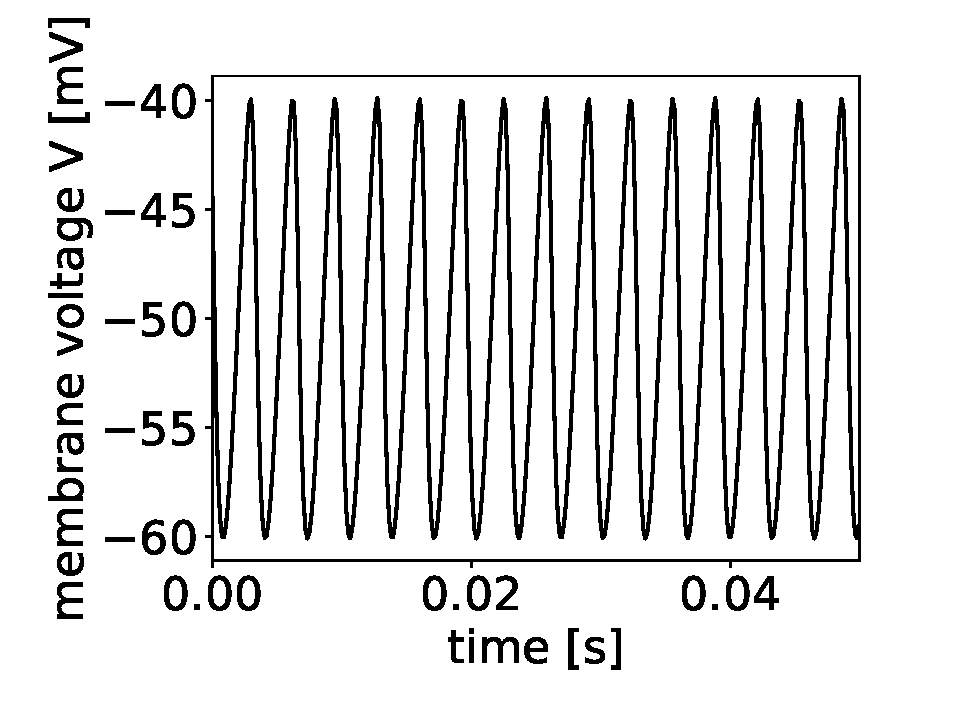
\includegraphics[scale=0.45]{inaprealanhopfunstablevtblack.pdf}}
	\caption{Evolution of the system on the unstable limit cycle. The left side shows the phase plane image and on the right one can see the membrane voltage over time.}
	\label{unstable} 
\end{figure}
Due to the numerical impossibility to put the system exactly onto the unstable limit cycle, any time-forward simulation starting on the unstable cycle will eventually collapse into either stable configuration, as shown in figure \ref{divergent}.
\begin{figure}[H]
	\subfigure[]{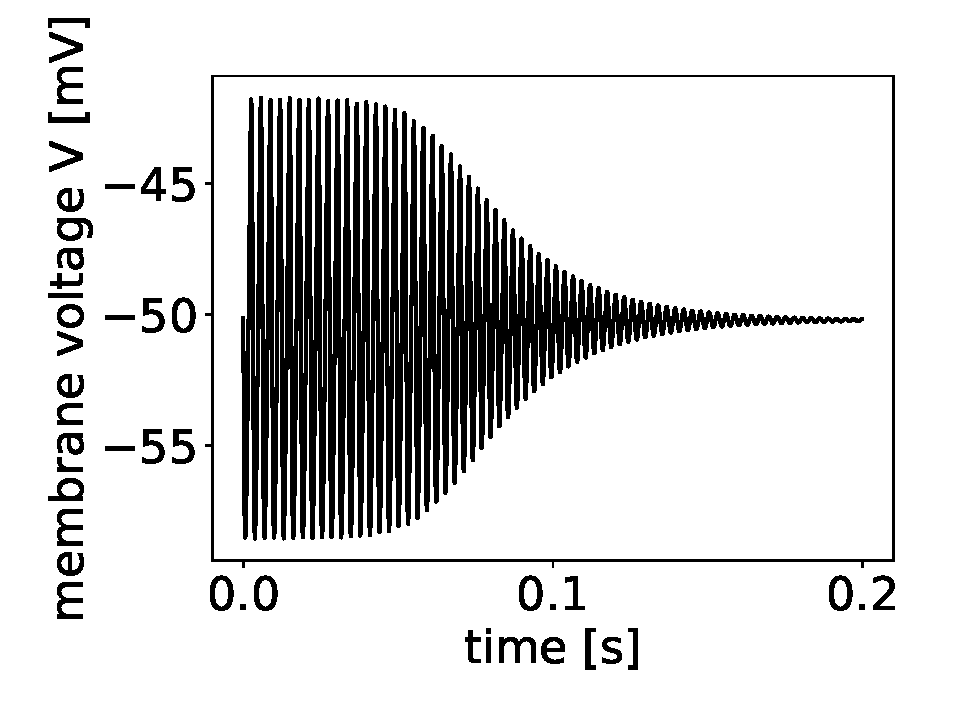
\includegraphics[scale=0.45]{inaprealanhopfnb2black.pdf}} 
	\subfigure[]{	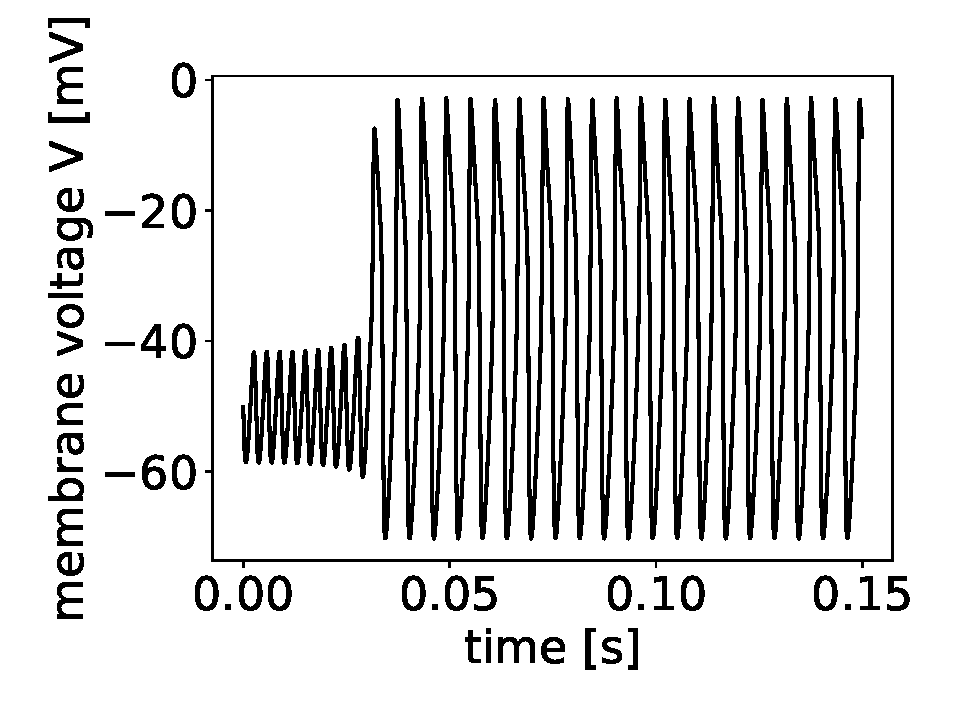
\includegraphics[scale=0.45]{inaprealanhopfunstable2black.pdf}}
	\caption{Evolution of the membrane voltage if the system is started near the unstable limit cycle. After a couple of circulations, the system quickly converges to a stable state.}
	\label{divergent} 
\end{figure}
\subsubsection{System with noise}

\begin{figure}[H]
	\subfigure[]{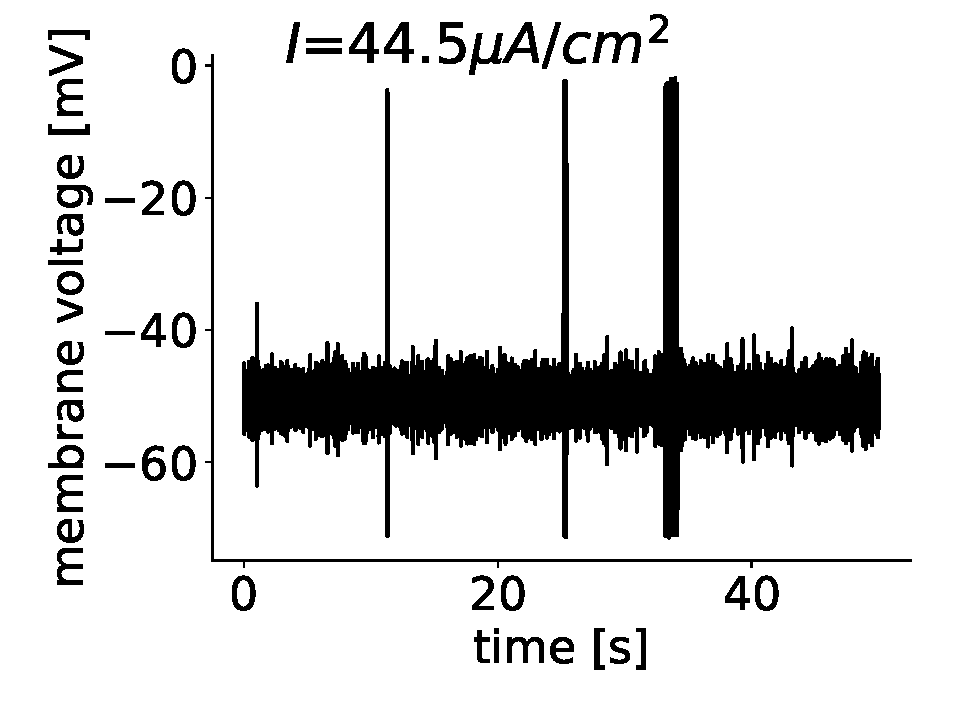
\includegraphics[scale=0.45]{realstateanhopf45full.pdf}} 
	\subfigure[]{	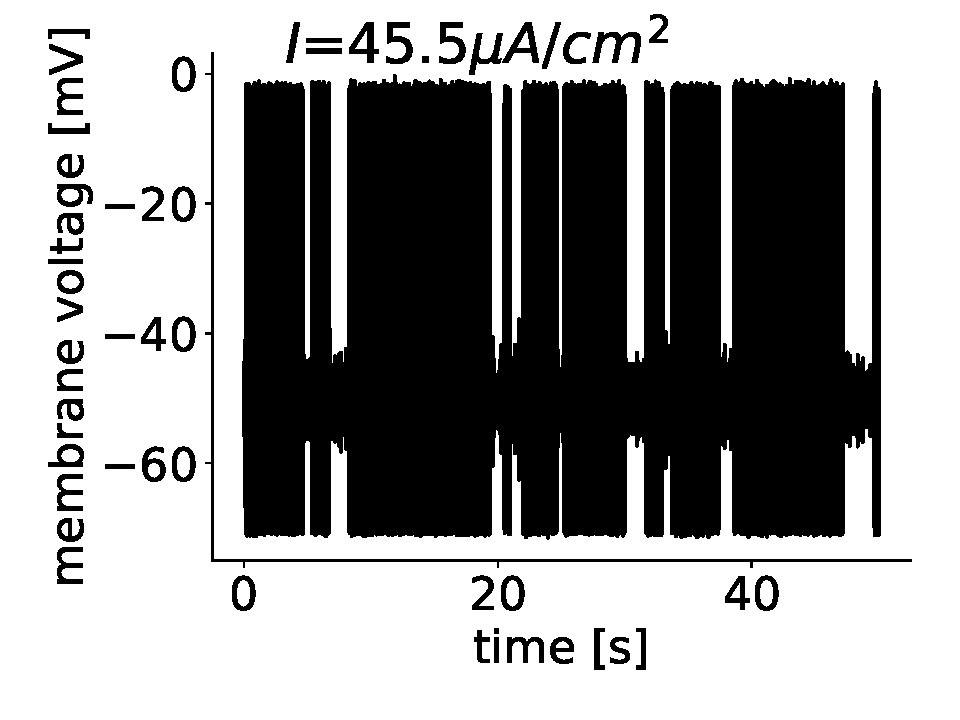
\includegraphics[scale=0.45]{realstateanhopf55full.pdf}}\\	\subfigure[]{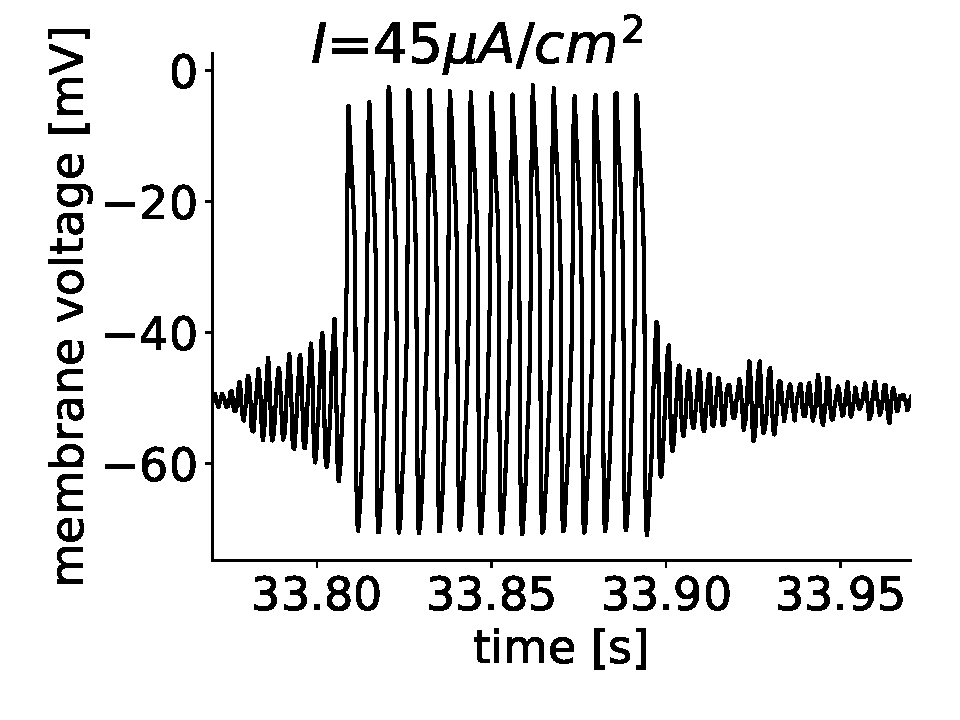
\includegraphics[scale=0.45]{realstateanhopf5sh3.pdf}} 
	\subfigure[]{	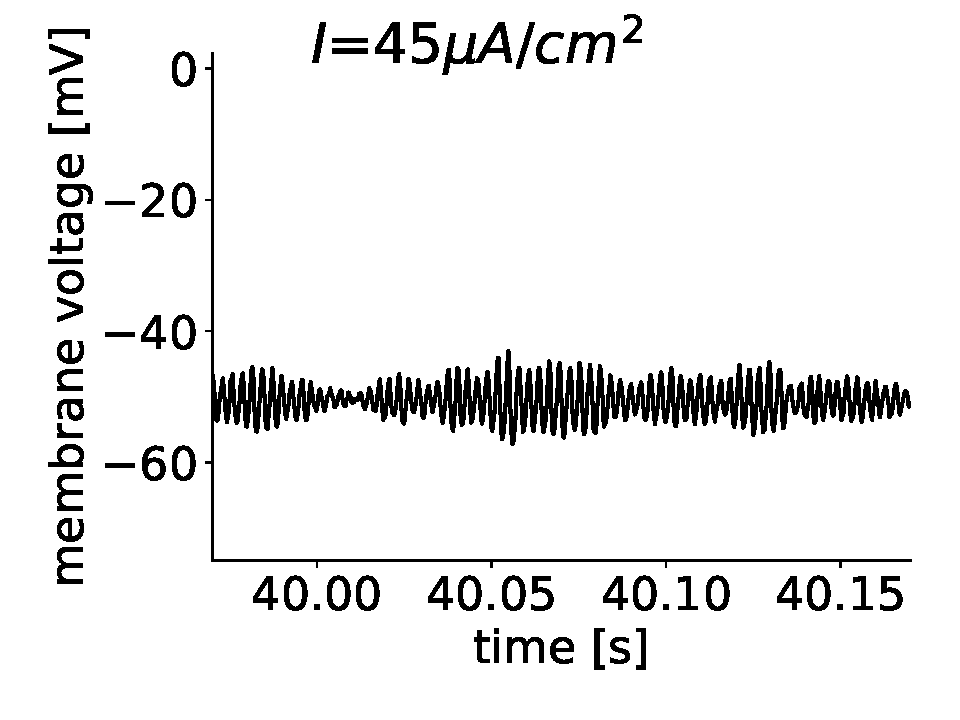
\includegraphics[scale=0.45]{realstateanhopf52sh.pdf}}
	\caption{Behavior of the membrane voltage for constant noise and changing bias current $I$ at $D=0.3$. On the bottom, one can see the behavior of the system with a higher time resolution. The small oscillations near equilibrum in (d) are subthreshold oscillations.}
	\label{ahnoise} 
\end{figure}
Considering that even in the noiseless system, the unstable limit cycle only lasts a few ms, it will not play any role in the noise-driven neuron. Therefore, the noise again just switches the system between spiking and resting state. The probability of each state can be influenced by tuning the bias current $I$, as can be seen in figure \ref{ahnoise}.
Over a range of $1\mu A/cm^2$, the neuron switches from barely spiking to basically only spiking. Due to the oscillatory properties of the system, small disturbances suffice to induce a change of state, if they occur at the right moment, as can be seen in 13 (c): Even though the state vector should be attracted to the stable focus, appropriate noise can slowly increase the amplitude of rotation until the spiking limit cycle is reached. In connection to this there exists another interesting phenomenon which is visible in (d): If the pulse amplitude is too small to make the neuron spike, it oscillates back to the focus with a high frequency, generating subthreshold oscillations.\\
The phenomenological investigation of the model will be concluded with a comparison between phase space and evolution over time.
\begin{figure}[H]
	\hspace*{-0.5cm}
	\subfigure[]{	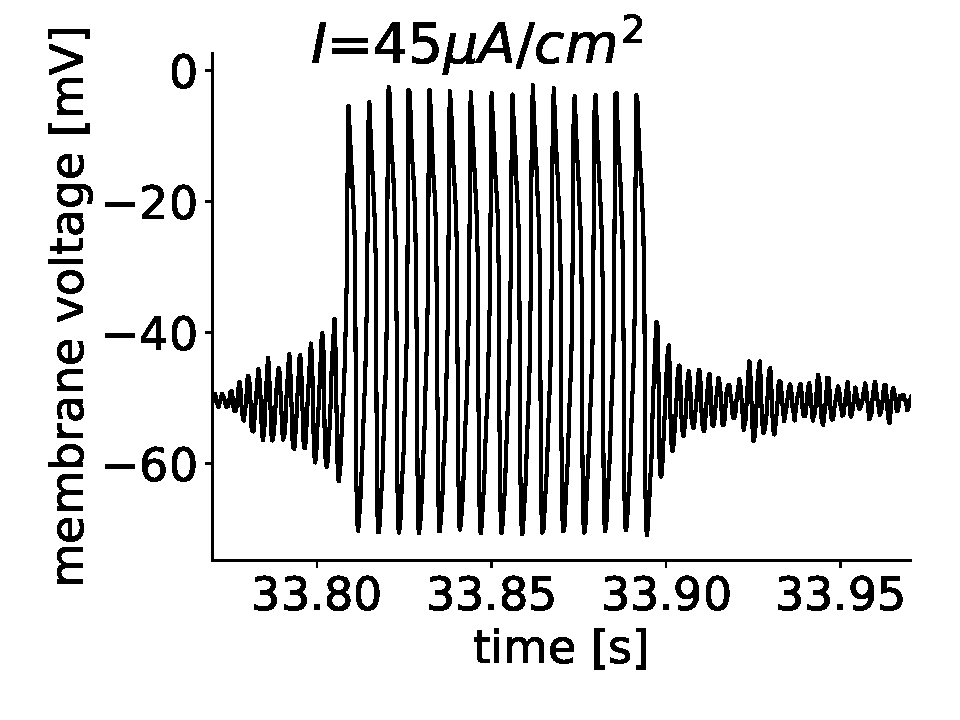
\includegraphics[scale=0.45]{realstateanhopf5sh3.pdf}}
	\subfigure[]{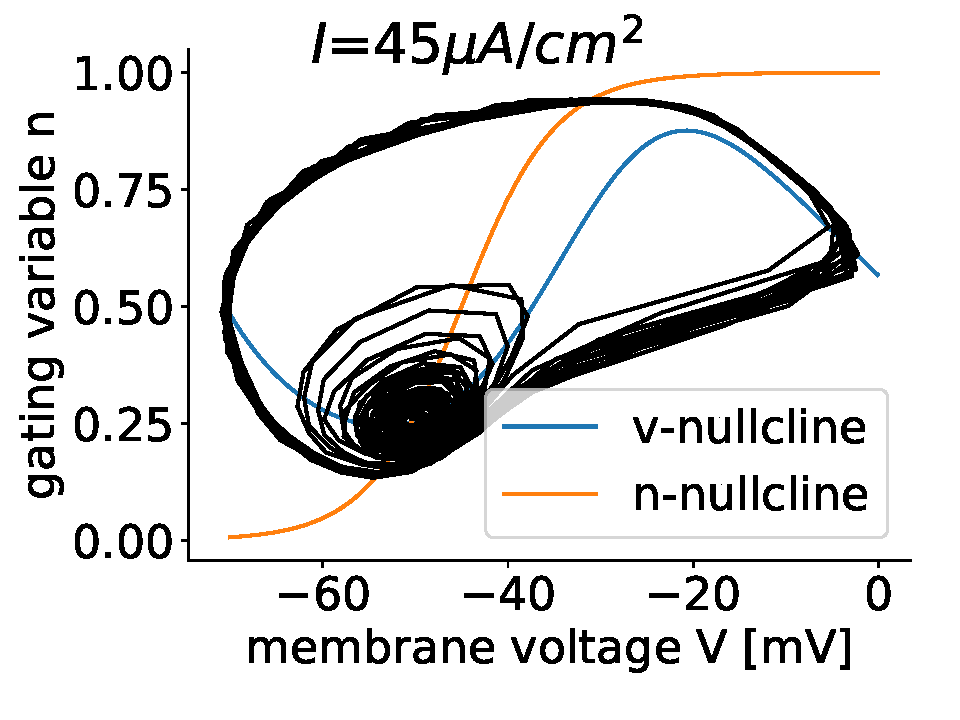
\includegraphics[scale=0.45]{inaprealanhopfreal5psh.pdf}}
	
	\caption{Evolution of the membrane voltage over time (left) and the corresponding phase space image.}
	\label{ppcompanhopf}
\end{figure}
Here, we see a quite stable limit cycle with amplitude variations of less than 5 mV, representing only a couple percent of the whole voltage range of the system. This is also clearly visible in the phase space: after crossing the V-nullcline near 0 mV in counterclockwise direction, all spiking trajectories practically overlap until they reach the n-nullcline at around 55 mV. On the other hand, the resting state is much more irregular than for the saddle-node bifurcation. The reason for this lies in the nature of the equilibrium point. When near the focus, the state vector does not directly approach it. Instead, it performs oscillations with shrinking radius. It is helpful to consider once more the eigenvalues of the Jacobian matrix. The ratio between real and imaginary part was about 1:46, meaning that the system near the equilibrium would roughly need to perform 10 oscillations to halve he radius of these oscillations. Therefore, the system only slowly approaches the resting point and can be easily influenced in either direction by noise.
\subsection{Rinzel model with saddle-node bifurcation}
The last model is a two-dimensional approximation of the Hodgkin-Huxley model, proposed by Rinzel in 1985 \cite{rinzel}. By assuming instantaneous $Na^+$ dynamics and expressing the two gating variables $h$ and $n$ by a single recovery variable $W$, Rinzel got the following model:
\begin{align*}
C\dot{V}&=I-g_{Na}m_\infty^3(V)(1-W)(V-E_{Na})-g_K(W/S)^4(V-E_K)-g_L(V-E_L)\\
\dot{W}&=\left[W_\infty(V)-W\right]/\tau(V)
\end{align*}
It has to be noted that for our simulations, white gaussian noise with intensity $D$ was added to the first equation.
However, the notation is almost similar to he $I_{na,p}+I_K$ model: $I$ denotes again the bias current, $C$ the capacitance, $V$ the membrane voltage, $g_i$ are conductances, $E_i$ the Nernst equilibrium potentials and $m_{\infty}$ the activation variable of the instantaneous $Na^+$ current. Inactivation of $Na^+$ and activation of $K^+$ are both governed by $W$. Its steady-state activation function $W_\infty$ is a linear combination of $n_\infty$ and $h_\infty$
\begin{align*}
W_\infty(V)=S\left(n_\infty(V)+S\left[1-h_\infty(V)\right]\right)/(1+S^2)\end{align*}
and $\tau$ comes from averaging the time constants of the gating variables
\begin{align*}
\tau(V)=\frac{5\exp[-(V+10)^2/55^2 ]+1}{3.82}
\end{align*}
The parameters were taken from the original Hodgkin-Huxley model:\\\\
$C=1$ , $g_L=0.3$ , $E_L=10$ , $g_{Na}=120$ , $E_{Na}=115$ , $g_K=36$ , $E_K=12$.\\\\
$S$ can be obtained from the resting values of $h$ and $n$
\begin{align*}
S=\frac{(1-h_\infty(0))}{n_\infty(0)}=1.27,
\end{align*}
and
\begin{align*}
k_\infty=\frac{\alpha_k}{\alpha_k+\beta_k}
\end{align*}
with
\begin{align*}
\alpha_n(V)&=0.01\frac{10-V}{\exp\left(\frac{10-V}{10}\right)-1}
&\beta_n(V)&=0.125\exp\left(\frac{-V}{80}\right)\\
\alpha_m(V)&=0.1\frac{25-V}{\exp\left(\frac{25-V}{10}\right)-1}
&\beta_m(V)&=4\exp\left(\frac{-V}{18}\right)\\
\alpha_h(V)&=0.07\exp\left(\frac{-V}{20}\right)
&\beta_h(V)&=\frac{1}{\exp\left(\frac{30-V}{10}\right)+1}
\end{align*}

\subsubsection{System without noise}
The first step in the phase plane analysis would again be determining the nullclines. Unfortunately, the variable $W$ not only occurs in linear form, but also in 4th power. This makes it analytically difficult to find a simple equation for the nullclines. Therefore, the nullclines were determined numerically.\\
Considering that this model is not a genuine two-dimensional neuron model, but just the result of a couple of simplifications carried out on the Hodgkin-Huxley model, the phase plane image can be understood as the 2-D projection of the 4-dimensional Hodgkin-Huxley model. Therefore, it comes as no surprise that the nullclines take on a more complex shape, consisting of a hill and an n-shaped part, both separated by a singularity at $V=10\text{mV}$. However, this does not change the fact that there are still 4 regions of different directions of motion, which are marked by arrows in figure \ref{rinzelnc}. 
\begin{figure}[H]
	\centering
	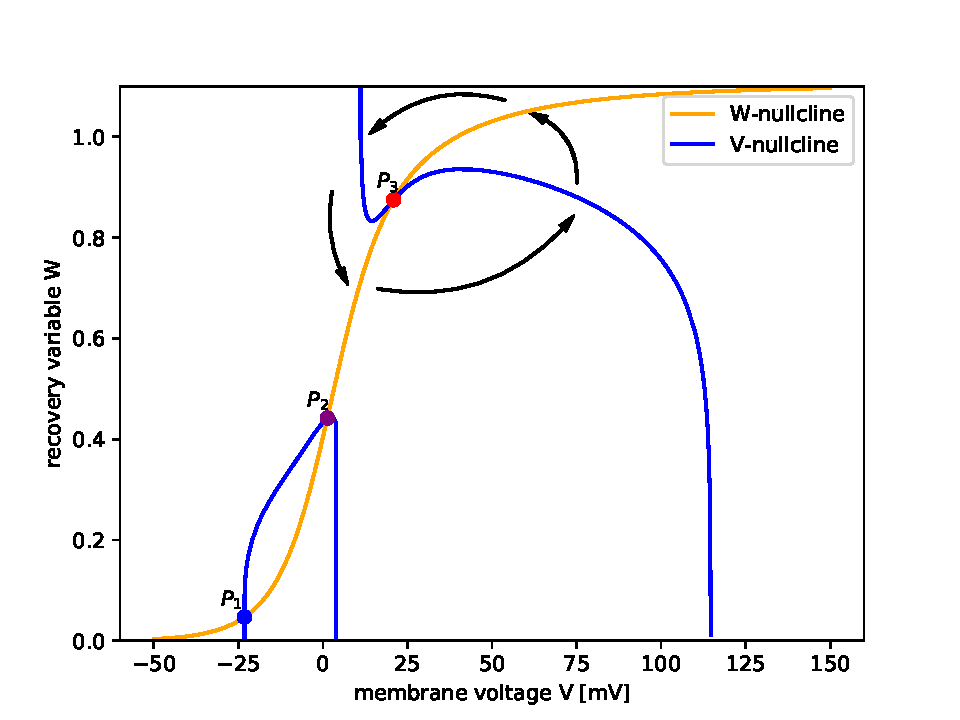
\includegraphics[scale=0.95]{rinzelclinesarrowwp.pdf}\caption{Nullclines of the Rinzel model with $I=-10$. The arrows indicate the direction of motion in the different regions.}
	\label{rinzelnc}
\end{figure}

The numerical evaluation of the Jacobian matrix yields:
\begin{align*}
\lambda_+(P_1)&\approx-0.3 & \lambda_-(P_1)&\approx-0.7\\
\lambda_+(P_2)&\approx 0.5& \lambda_-(P_2)&\approx -1.4\\
\lambda_+(P_3)&\approx 6.3& \lambda_-(P_3)&\approx 0.5
\end{align*}
This means that there is a stable node at $P_1$, a saddle at $P_2$ and an unstable node at $P_3$. Upon increase of $I$, the hill will move downwards, eventually leading to a merger of $P_1$ and $P_2$ at $I\approx -5.91$ when the system undergoes a saddle-node bifurcation and is no longer in the bistable regime.\\
When it is in the bistable regime, there are two sets of initial conditions, leading either to quiescence or repetitive firing as shown in figure \ref{subfigrinzel}.\\
Apparently, it is only a matter of a couple tens of microseconds to reach a stable configuration: the system converges exponentially to the stable equilibrium or after an initial larger spike, it goes around on the spiking limit cycle, respectively.
\begin{figure}[H]
	\subfigure[]{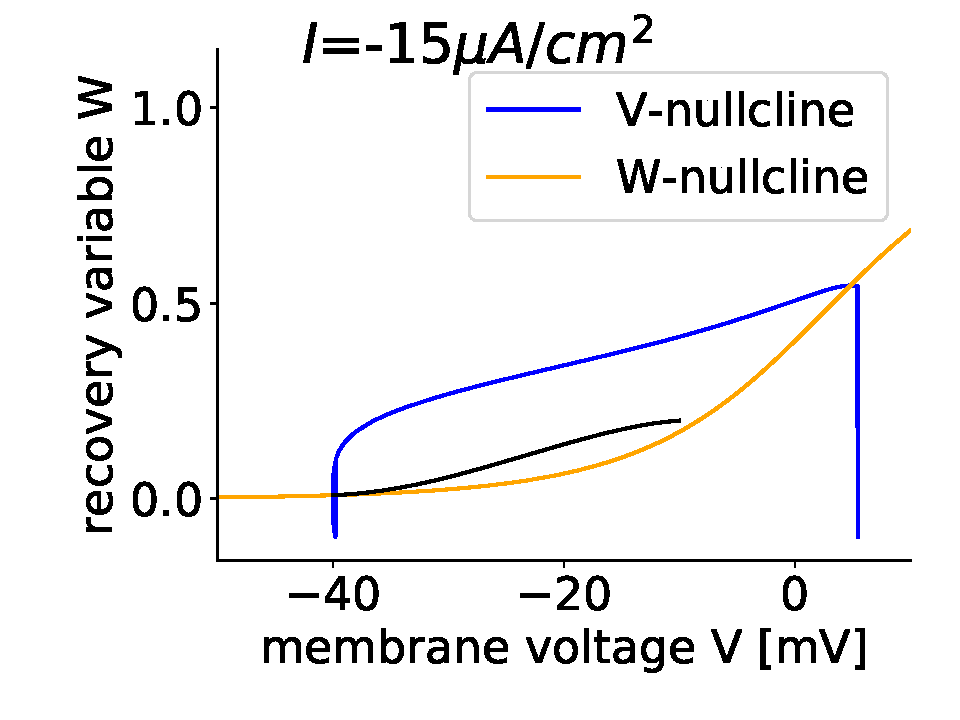
\includegraphics[scale=0.45]{realstatedetrinzelpnb2wnblack.pdf}} 
	\subfigure[]{	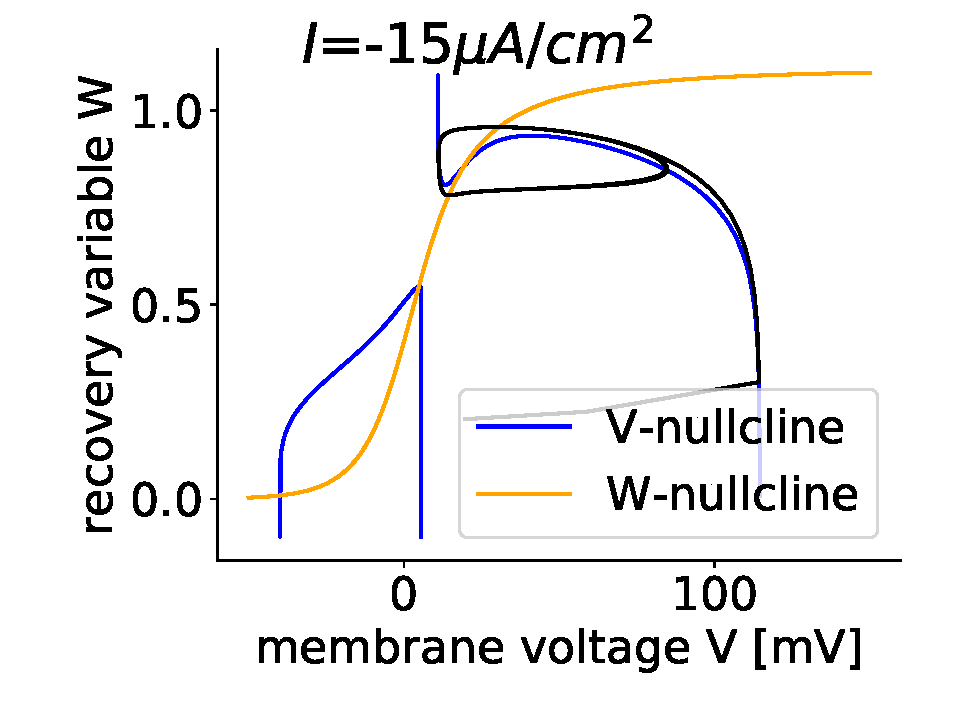
\includegraphics[scale=0.45]{realstatedetrinzelpnbwnblack.pdf}}\\	\subfigure[]{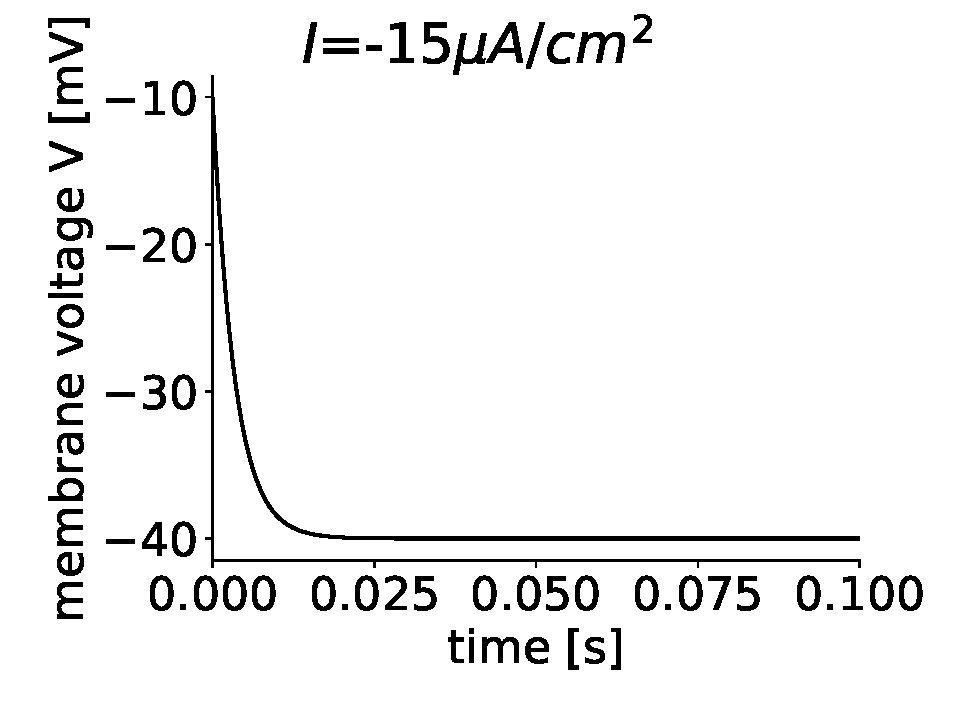
\includegraphics[scale=0.45]{realstatedetrinzelpnb2.pdf}} 
	\subfigure[]{	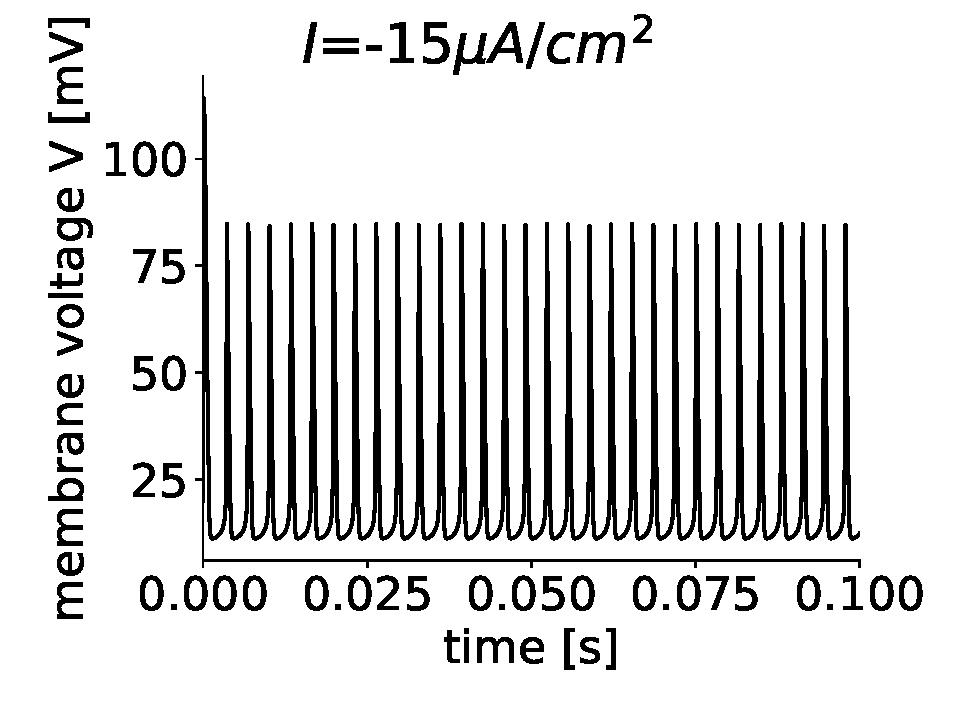
\includegraphics[scale=0.45]{realstatedetrinzelpnb.pdf}}
	\caption{Evolution of the phase vector (first row) and the membrane voltage over time (second row). The left side shows the evolution of the system with resting ICs, and on the right one can see the behavior under spiking ICs.}
	\label{subfigrinzel} 
\end{figure}


\begin{figure}[H]
	\hspace*{-0.5cm}
	\subfigure[]{	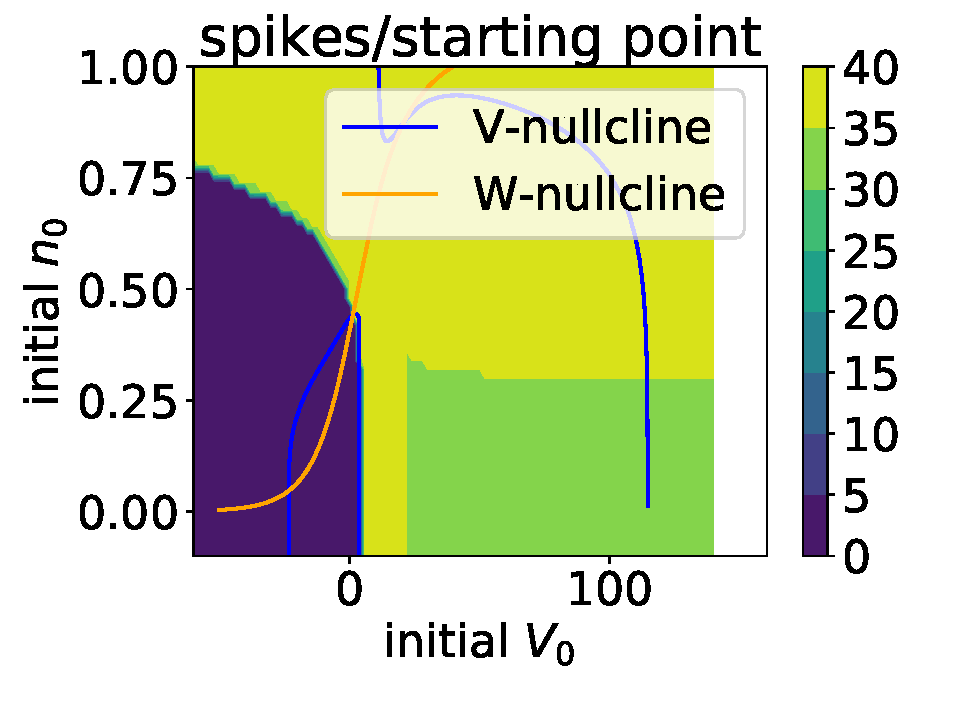
\includegraphics[scale=0.45]{contourrinzela12shalt3.pdf}}
	\subfigure[]{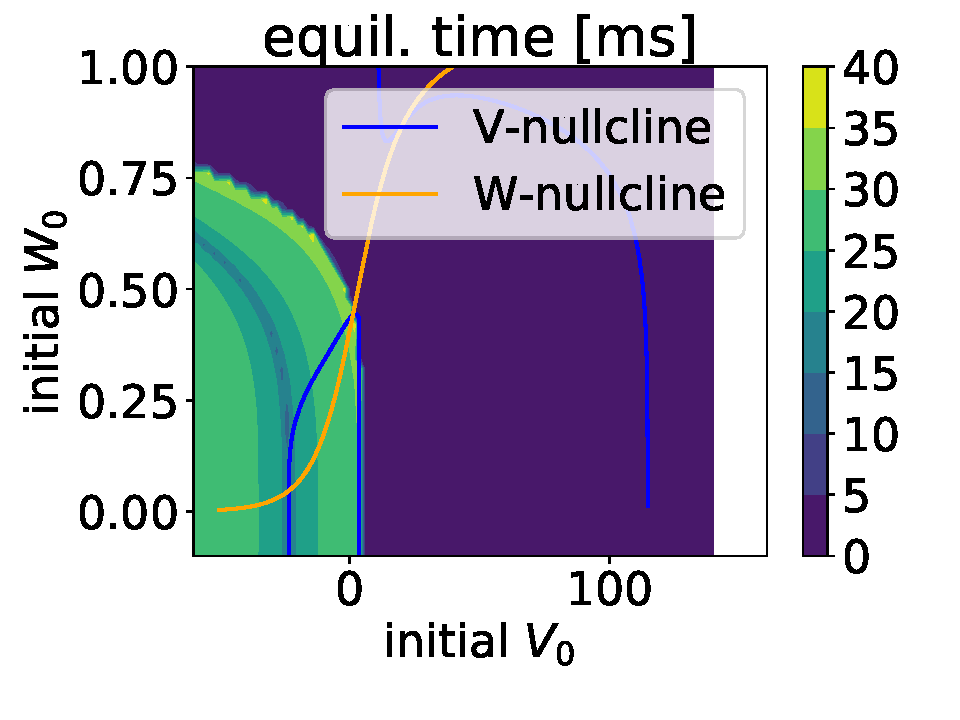
\includegraphics[scale=0.45]{contourrinzela12time.pdf}}
	
	\caption{Phase plane image of the neuron model with $I=-10$ and no noise. Each point represents a specific combination of starting parameters. The left plot shows the number of spikes over a short period of time and for the right figure, the equilibration times for both states were measured. Irregularities arise from the finite resolution of the $V_0$-$n_0$-lattice.}
	\label{twodomrinzel}
\end{figure}
The two sets of initial conditions can once again be distinguished by letting the system evolve without noise from different starting points.\\
Even though the nullclines have a more complex shape, the sets of initial conditions are again separated by a single line.
Interestingly, the plots in figure \ref{twodomrinzel} look inverse to each other. This means that the firing state is reached much faster than the resting state, almost independent of the starting point. Similarly to the $I_{Na,p}+I_K$-model, the border goes, as expected, through the saddle point.

\subsubsection{System with noise}
Now that the model has been understood in the phase plane, the influence of noise can be investigated.
\begin{figure}[H]
	\subfigure[]{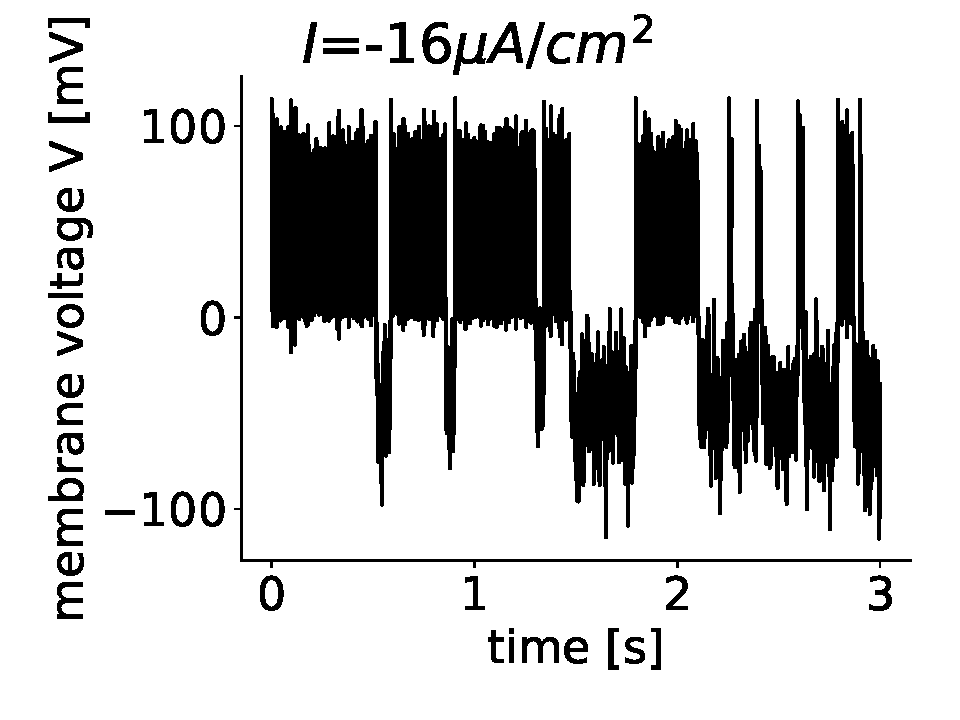
\includegraphics[scale=0.45]{realstatedetrinzel16100.pdf}} 
	\subfigure[]{	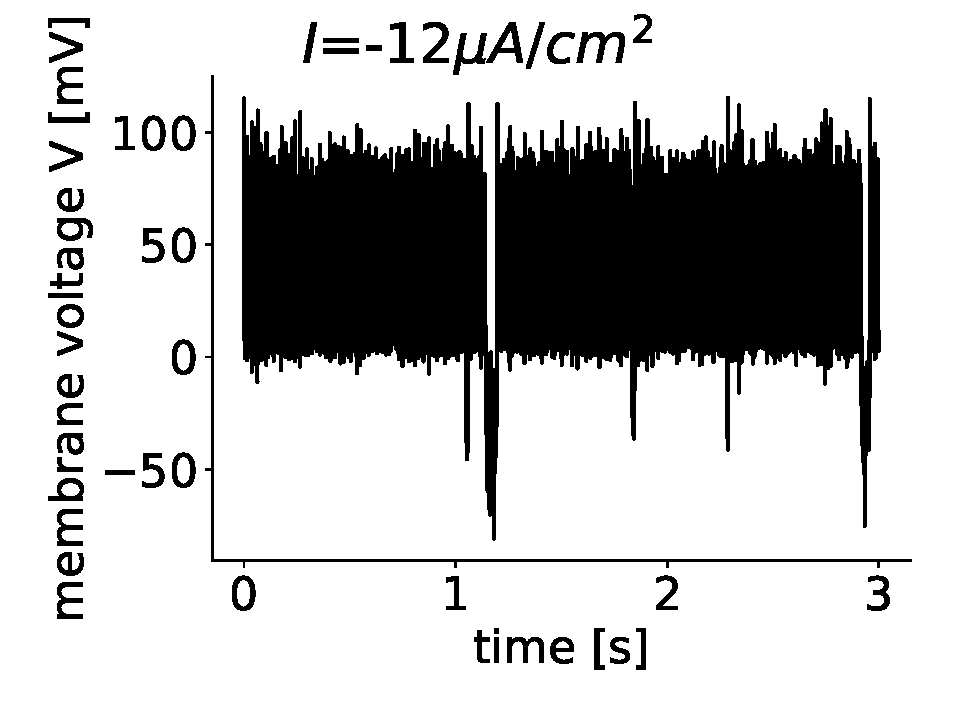
\includegraphics[scale=0.45]{realstatedetrinzel12100.pdf}}\\	\subfigure[]{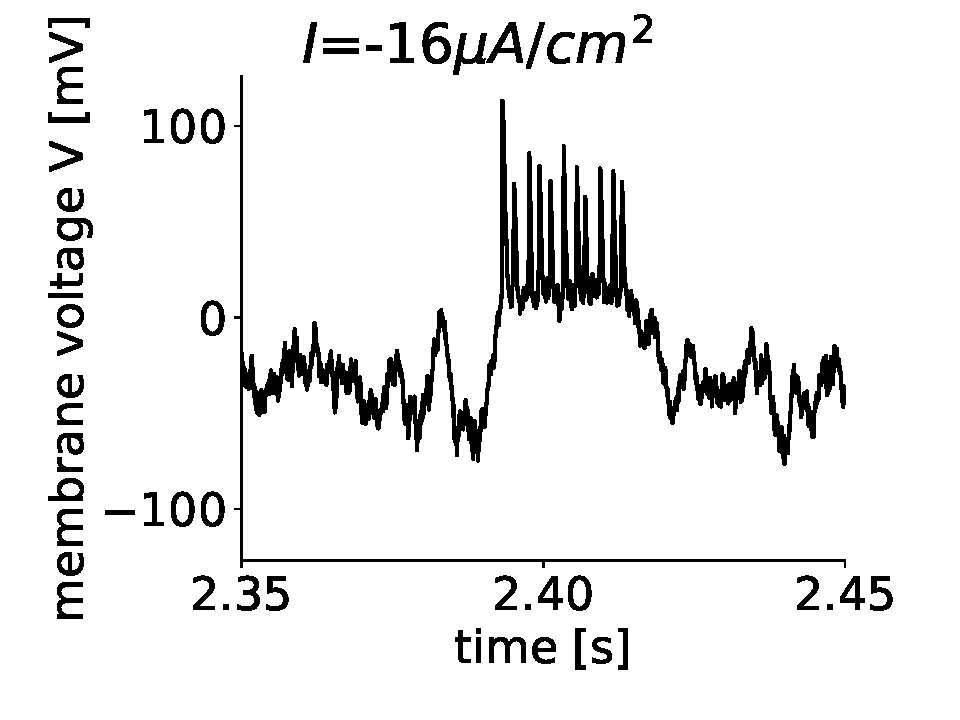
\includegraphics[scale=0.45]{realstatedetrinzel16100sh2.pdf}} 
	\subfigure[]{	\includegraphics[scale=0.45]{realstatedetrinzel12100sh.pdf}}
	\caption{Behavior of the membrane voltage for constant noise and changing bias current $I$ at $D=100$. On the bottom, one can see the behavior of the system with a higher time resolution.}
	\label{rinzelnoise} 
\end{figure}
Here, too, the bias current $I$ is the parameter that controls whether resting or spiking state is preferred. At intermediate $I$, the neuron fires irregularly and the noise has a high impact on its behavior. At high bias currents, the neuron barely goes into the resting state, and even that only for a short period of time before going back to tonic spiking. The major impact of noise in this regime lies in the modulation of firing rate and spike height, clearly visible in \ref{rinzelnoise} (d). This is a major difference to the other neuron models, where we observed a very regular firing with no visible variations of the firing rate. This might also have an influence on the count statistics and other relevant quantities as they are presented in section \ref{quant}.

\begin{figure}[H]
	\hspace*{-0.5cm}
	\subfigure[]{	\includegraphics[scale=0.45]{realstatedetrinzel16100sh2.pdf}}
	\subfigure[]{\includegraphics[scale=0.45]{realstatedetrinzelp16100shnn.pdf}}
	
	\caption{Evolution of the membrane voltage over time (left) and the corresponding phase space image. The blue curves represent the V-nullcline, the orange one is the n-nullcline. }
	\label{ppcomprinzel}
\end{figure}
The noise-induced fluctuations are illustrated by trajectories in the phase plane. Here, one can see that resting and spiking state both are subject to variations in both variables. Considering that just in figure \ref{ppcomprinzel} there are five distinct trajectories near the limit cycle, there does not seem to be such a thing as a stable cycle. It comes as no surprise that the resting state is characterized by continuous jittering in W- and V-direction. The stable equilibrium is now much closer to $V_{1/2}$ of the W-nullcline than in the first model, so we can expect changes in both variables. Lastly, the transition from resting to spiking happens quite regularly, once the V-nullcline is crossed. However, the opposite transition is noisy the whole time. This indicates that the transition to the resting takes a longer time and therefore might also be less likely, as was already observed in the system without noise.\\\\
In conclusion, all three two-dimensional bursting neuron models display the same characteristics as the underdamped Brownian particle in a tilted potential. They have bistable firing dynamics in the form of a state of repetitive spiking, corresponding to the running state and a resting state without spiking that can be associated with the locked state. Furthermore, transitions between the states can be induced by noise. Therefore, we expect to find similar count statistics and giant diffusion for these systems as well. If this assumption is actually valid will be examined in the following chapter.
\subsection{Quantities of interest}\label{quant}
%\subsubsection{System without signal}
In the context of Brownian Motion, there were two characteristic quantities: the ensemble of particles moves with a mean velocity
\begin{equation}
\left\langle v\right\rangle =\lim_{t\rightarrow\infty}\frac{\left\langle x(t)-x(0) \right\rangle}{t}
\end{equation}
and is subject to a diffusive spread around this average flow that can be described by the effective diffusion coefficient
\begin{equation}
D_{eff}=\lim_{t\rightarrow\infty}\frac{\left\langle x^2(t) \right\rangle-\left\langle x(t)\right\rangle ^2}{2t}
\end{equation}
In the context of neuron models, similar quantities can be defined. The most important event with regard to signal transmission is the generation of a spike. Therefore, it is often useful to approximate the voltage curve by a spike train where every spike is assumed to be a Dirac-delta function,
\begin{equation}
x(t)=\sum_{i}\delta(t-t_i)
\end{equation}
An important quantity is the spike count $N(t)$ which describes the number of spikes fired after a time $t$. This can be easily found by integrating the spike train over time:
\begin{equation}
N(t)=\int_{0}^{t}dt'x(t')=\sum_{t_i<t} 1
\end{equation}
Instead of the mean velocity, one can ask for the average firing rate
\begin{equation}\label{vdef}
\left\langle v\right\rangle =\lim_{t\rightarrow\infty}\frac{\left\langle N(t) \right\rangle}{t}
\end{equation} 
and the diffusive spread of the spike count
\begin{equation}\label{deffdef}
D_{eff}=\lim_{t\rightarrow\infty}\frac{\left\langle N^2(t) \right\rangle-\left\langle N(t)\right\rangle ^2}{2t}
\end{equation}
A more common way to measure spiking variability in neurons is the Fano factor, which can be calculated by dividing the variance of the spike count by its mean value:
\begin{align*}
F=\frac{\left\langle \Delta N^2(t) \right\rangle}{\left\langle N(t)\right\rangle}
\end{align*}
Using equations \ref{deffdef} and \ref{vdef}, the Fano factor can be related to firing rate $\left<v\right>$ and $D_{eff}$:
\begin{align*}
F=\frac{2D_{eff}}{\langle v\rangle}
\end{align*}
%\subsubsection{System with signal}\label{sws}
When bistable neurons are subjected to a periodic stimulus, they should change their firing pattern accordingly. This is best visible in the power spectrum of the spike train, 
\begin{equation}
S(f)=\lim_{T\rightarrow\infty}\frac{\langle|\tilde{x}|^2\rangle}{T}
\end{equation}
$\tilde{x}$ is the Fourier transformation of the spike train. The quality of signal transmission is measured by the signal-to-noise ratio (SNR). The stronger the system changes its behavior in response to the signal, the higher should be the signal-to-noise ratio. It is calculated by comparing the spectral power at signal frequency $f_s$ with the noise, i.e. the spectral power $S_{bg}$ of the background,
\begin{equation}
SNR=\frac{S(f_{s})-S_{bg}(f_{s})}{S_{bg}(f_{s})}
\end{equation}
The background power can be obtained by averaging the spectral power of a couple of points near the signal frequency while excluding the signal frequency itself. 
\\
In the case of a weak and very slow signal, some simplifications can be made. First, it can be assumed that apart from a peak at the signal frequency, the power spectrum looks similar to the unperturbed one, yielding $S_{bg}(f_s)=S_0(f_s)$. In the low-frequency-limit, this simplifies even further to $S_{0}(f_s)=S_0(0)$. At long simulations times, the power spectrum can be related to the effective diffusion coefficient via $S_0(0)=2D_{eff}$\cite{deffspec}, which was used in equation \ref{snrweaksig}. Lastly, the susceptibility $\chi$ which quantifies the modulation of the firing rate can be approximated with the derivative of the firing rate $\left<v\right>$ by the control parameter, in our case this is the bias current $I$. All in all, one then gets
\begin{align}\label{snrweaksig}
SNR=\frac{\epsilon ^2T}{4}\frac{|\chi(\omega)|^2}{S_0(\omega)}=\frac{\epsilon^2T|d\left<v\right>/dI|^2}{8\cdot D_{eff}}
\end{align}
where $\epsilon$ is the signal amplitude and $T$ the total simulation time.
%\subsection{giant diffusion}
%The term \glqq giant diffusion \grqq is short for \textit{Giant Enhancement of (thermal) diffusion} which was first observed around the turn of the millennium for Brownian Particles in a tilted periodic potential\cite{td}\cite{ga}\cite{dit}\cite{gd}. In general, these particles exhibit two stable velocity states. They can be \glqq trapped\grqq in a potential minimum - this is referred to as the \textit{locked state} - or they can be in the \textit{running state}. A particle gets into the running state if it has managed to overcome a hill and the frictional loss is low enough so that it is able to pass the adjacent hills as well. In the case of large friction or a strongly tilted potential, however, only one of these two states is present. If the potential is tilted in such a way that both states exist and the probabilities to be in either state are similar, many switchings between the states will occur. In the weak-noise-limit, half of the particles will be mainly in the locked state, while for the others the running state prevails. This behavior leads to diverging diffusion coefficients known as giant diffusion.
%\subsection{giant diffusion of Brownian Particles}
%First observed by the botanist Robert Brown in 1828\cite{bm}, the term \textit{Brownian Motion} describes the irregular movement of particles in a viscous medium, whose apparently random changes of direction are caused by collisions with smaller particles or molecules.
%\\
%Ordinary Brownian Motion obeys a simple linear Langevin-equation:
%\begin{align*}
%\text{m}\dot{v}=-\lambda v+\xi(t)
%\end{align*}
%The evolution of the velocity $v$ of the particle is affected by a linear friction term with coefficient $\lambda$ and a random force $\xi(t)$. \\
%\\ 
%In the following, two different systems with Brownian Motion dynamics exhibiting giant diffusion are presented. These were the motivation for my research on bursting neuron models.
%\subsubsection{Active Brownian Particles}
%Active Brownian Motion can be observed on small organisms, like bacteria or cells, which are able to move on their own. In order to model the behaviour of such an object, a more general friction term needs to be introduced into the Langevin-equation:
%\begin{align*}
%\dot{v}=-f(v)+\xi(t)
%\end{align*}
%Here, the noise was assumed to be additive and the mass was omitted due to clarity.
%An accurate description of the self-propulsion can be accomplished by choosing the function $f$ in such a way that it attains negative values at small velocities and becomes greater than zero at large speed. Thus, at small velocities the particle will accelerate and with increasing velocity, regular friction will start to affect its motion.
%\\
%A system like this was studied by Lindner and Nicola in 2008\cite{abp}. They chose a cubic function for the friction term, $f(v)=v-v^3+F$, allowing them to write the equation of motion in terms of a quartic velocity potential $U(v)$:
%\begin{equation}
%\dot{v}=-U'(v)+\xi(t)
%\end{equation}
%with $U(v)=\frac{1}{4}v^4-\frac{1}{2}v^2-Fv$.
%\begin{figure}[H]
%	\centering
%	\includegraphics[scale=1]{velpot.pdf} 
%	\caption{tilted velocity potential of an Active Brownian Particle}
%	\label{velpot}
%\end{figure}
%This potential shows two minima at $v_\pm$, representing the stable velocity states \glqq forwards\grqq and \glqq backwards\grqq, and a maximum at $v_0$. In order to transition from $v_\pm$ into the other state, the particle needs to overcome a barrier of height $\Delta U\pm$.  
%\\
%Their simulations revealed a certain region of bias forces $F$, in which giant diffusion occurred.
%\begin{figure}[H]
%	\centering
%	\includegraphics[scale=0.5]{mess08.png}\caption{Simulation of velocity and effective diffusion coefficient for Active Brownian Particles underlying a tilted velocity potential,taken from \cite{abp}}
%	\label{abpsim}
%\end{figure}
%Inside this region, the diffusion coefficients increase with decreasing noise intensity, while they decrease outside of this region. In other words, in the weak noise limit, the diffusion coefficients diverge in the critical region and vanish outside of it. The critical force lies at the border of this region and emerges from the intersection points of the diffusion coefficients for different noise levels. A simple criterion could be found for these intersection points: at the critical force, one potential barrier is twice as high as the other potential barrier. 
%Furthermore, it is remarkable that the reliable directed transport which takes place outside of the critical region appears much earlier than the monostability of the velocity potential, which is a obviously only a primitive criterion for reliable transport in one direction. 
%The mean velocity displays a more regular behavior. It is almost constant at a value less than zero up to small negative forces, then undergoes a sharp increase to a positive value and barely changes afterwards. They intersect as well, approximately at the position where the diffusion coefficient gets maximal.
%\subsubsection{Regular Brownian Particles in a tilted periodic potential}
%On their own, ordinary Brownian Particles do not exhibit bistable velocity dynamics which may lead to giant diffusion. But as mentioned before, this can be done by adding a periodic potential to the equation of motion:
%\begin{equation}
%\dot{v}=-\gamma v-U'(x)+\sqrt{2\gamma kT}\xi(t)
%\end{equation}
%with $U(x)=-Fx-d\cos(x)$. This system was discussed with respect to giant diffusion in a paper by Lindner and Sokolov from 2016\cite{bpp}. Now, in contrast to the Active Brownian Particle, the evolution of the system is not governed by a velocity potential, but by a spatial potential:
%\begin{figure}[H]
%	\subfigure[]{\includegraphics[width=0.5\textwidth]{veldynupper.png}} 
%	\subfigure[]{\includegraphics[width=0.5\textwidth]{veldynlower.png}} 
%	\caption{Figure (a) visualizes the motion of a Brownian Particle in a periodic potential, on the right one can see the bistable velocity dynamics. The oscillations thereby arise from local extrema of the potential.}
%	\label{veldyn} 
%\end{figure}
%Also for the Brownian Particles in a cosine potential, there was a finite range of bias forces, for which giant diffusion could be observed:
%\begin{figure}[H]
%	\centering
%	\includegraphics[scale=0.5]{nbpsim1.png}\caption{Simulation of velocity and effective diffusion coefficient for Brownian Particles in a tilted periodic potential,taken from \cite{bpp}}
%	\label{anbpsim}
%\end{figure}
%Again, all curves of the diffusion coefficient intersect at two points and diverge in between those points for decreasing noise intensities while going to zero on the outside and the velocity curves intersect approximately at the maximum of the diffusion coefficient. And also here the region of giant diffusion is much smaller than the range of bias forces, where both states coexist. Two other variables that help characterize the system are the transition rates between the states, that is from the locked to the running state and vice versa. Even though there didn't exist actual potential barriers, these turned out to obey an Arrhenius or Kramers law, respectively, as can be seen from an Arrhenius plot:
%\begin{figure}[H]
%	\centering
%	\includegraphics[scale=0.5]{kramerfit.png}\caption{Fits of the transition rates with both an Arrhenius and a Kramers law, taken from \cite{bpp}}
%	\label{bparr}
%\end{figure}
%In this example, the Arrhenius fit as well as the Kramers fit yield good agreements with the data. From these fits one can extract effective potential barriers. The relation found for the potential barriers of the Active Brownian Particle can be tested by plotting the effective barriers and twice their value:
%\begin{figure}[H]	\includegraphics[scale=0.5]{barrierplot.png}\caption{Plot of the effective potential barriers. The dotted curves are simply twice the solid curves of the same color. This plot is taken from \cite{bpp}}
%\end{figure}
%The plot shows that the points where one potential barrier equals twice the other roughly correspond to the critical forces, so the criterion applies as well to this case, where no potential barriers were present and only effective barriers could be calculated.
%\subsection{Two-state theory}\label{tst}
%In the case of low noise intensity, the transition times between the locked state and the running state will be much shorter than the periods of time that the particle stays in one of the two states. That is why it is practical to describe the behavior of the system in this regime with a two-state model. The following derivation applies to the Brownian Particle in a tilted periodic potential. The transition rates are assumed to obey an Arrhenius law:
%\begin{align*}
%r_{\pm}=r_{0,\pm}\exp\left(-\frac{\Delta U_{\pm}}{D}\right)
%\end{align*}
%where $r_-$ denotes the transition rate from locked to running state, and $r_+$ the rate for the other transition. $\Delta U_{\pm}$ is the corresponding potential barrier and $D$ the noise intensity. The effective diffusion coefficient can be calculated from the velocity $v_0$ in the running state and the transition rates: 
%\begin{align*}
%D_{\text{eff}}=\frac{v_0^2 r_+r_-}{(r_++r_-)^3}
%\end{align*}
%The first task is to find the intersection points of the diffusion coefficients. At these points, the diffusion coefficients become independent of the noise intensity.
%It is
%\begin{align*}
%D_{\text{eff}}&=\frac{v_0^2r_{0,+}r_{0,-}\exp\left(-\frac{\Delta U_++\Delta U_-}{D}\right)}{\left[r_{0,+}\exp(\frac{-\Delta U_+}{D})+r_{0,-}\exp\left(\frac{-\Delta U_-}{D}\right)\right]^3}\\&=\frac{v_0^2r_{0,+}r_{0,-}}{\left[r_{0,+}\exp\left(-\frac{3\Delta U_+-\Delta U_+-\Delta U_-}{3D}\right)+r_{0,-}\exp\left(-\frac{3\Delta U_--\Delta U_+ -\Delta U_-}{3D}\right)\right]^3}\\&=\frac{v_0^2r_{0,+}r_{0,-}}{\left[r_{0,+}\exp\left(-\frac{2\Delta U_+-\Delta U_-}{3D}\right)+r_{0,-}\exp\left(-\frac{2\Delta U_--\Delta U_+}{3D}\right)\right]^3}
%\end{align*}
%In the limes $D\rightarrow 0,\Delta U_+>U_-$ the first term in the denominator vanishes, resulting in:
%\begin{align*}
%D_{\text{eff}}=\frac{v_0^2r_{0,+}}{r_{0,-}^2}\exp\left(-\frac{\Delta U_+-2\Delta U_-}{D}\right)
%\end{align*}
%Under the assumption that the prefactors change slowly in comparison to the exponential function, the following condition arises:
%\begin{align*}
%\Delta U_+=2\Delta U_-
%\end{align*}
%Due to symmetry of the problem, the opposing case $D\rightarrow 0,\Delta U_+<U_-$ yields:
%\begin{align*}
%\Delta U_-=2\Delta U_+
%\end{align*}
%In both cases, one potential barrier is twice as high as the other one.\\
\subsection{Two-state theory}\label{tst}
%\subsubsection{Fano factor in weak noise limit}
In the introduction we were able to describe the firing behavior of the neuron by using an Arrhenius-like description of the transition rates:
\begin{align*}
r_{\pm}=r_{0,\pm}\exp\left(-\frac{\Delta U_{\pm}}{D}\right)
\end{align*}
This allowed us to calculate the effective diffusion coefficient:
\begin{align*}
D_{\text{eff}}=\frac{v_0^2 r_+r_-}{(r_++r_-)^3}
\end{align*}
As mentioned before, the Fano factor $F$ is a more common way to describe the spiking characteristics of a neuron. Therefore, we will examine whether the Fano factor displays similar features in the weak noise limit as the effective diffusion coefficient. As 
\begin{align*}
F=\frac{2D_{\text{eff}}}{\langle v\rangle}
\end{align*}
an expression for the average firing rate is required to compute $F$. Taking into account that the firing rate is zero when the particle is in the locked state, one finds the following formula for the total mean firing rate:
\begin{align*}
\langle v\rangle=v_0\frac{r_-}{r_++r_-}
\end{align*}
Therefore
\begin{align*}
F=\frac{2v_0r_+}{(r_++r_-)^2}=\frac{2v_0r_{0,+}\exp\left(\frac{-\Delta U_+}{D}\right)}{\left(r_{0,+}\exp\left(\frac{-\Delta U_+}{D}\right)+r_{0,-}\exp\left(-\frac{\Delta U_-}{D}\right)\right)^2}
\end{align*}
Having access to the transition rates, this formula allows to find a description of the Fano factor. In order to make general statements about $F$, one can again take a look at possible intersection points of all curves. Similarly to the approach in the introduction, these can be found by looking for a vanishing $D$-dependence in the low-noise limit.\\
For $\Delta U_+ > \Delta U_-$, it is:
\begin{align*}
F=\frac{2v_0r_{0,+}}{r_{0,-}^2}\exp\left(-\frac{\Delta U_+-2\Delta U_-}{D}\right) 
\end{align*}
Neglecting the prefactors with regard to the exponential term, the $D$-dependence disappears if the exponent becomes zero, yielding 
\begin{align*}
\Delta U_+=2\Delta U_-
\end{align*}
The case $\Delta U_+ < \Delta U_-$ gives:
\begin{align*}
F=\frac{2v_0}{r_{0,+}}\exp\left(-\frac{\Delta U_+-2\Delta U_+}{D}\right)
\end{align*}
This simply reduces to the criterion
\begin{align*}
\Delta U_+=0
\end{align*}
The intersection point for $\Delta U_+ > \Delta U_-$ stays the same while at the other critical point the potential barrier from running to locked state needs to vanish. As the latter condition violates the requirements for the application of the two-state theory - because only one state would exist in this case - the second intersection point can not be determined via this two-state model. This implies that the Fano factor $F$ only has one intersection point.\\\\
%\subsubsection{Behavior of SNR}
Formula (\ref{snrweaksig}) allows to compute the SNR from $D_{eff}$ and the derivative of the firing rate. As the effective diffusion coefficient can already be expressed via the transition rates, only $d\left<v\right>/dI$ is missing. This can be found as follows:
\begin{align*}
\frac{d\left<v\right>}{dI}&=\frac{d}{dI}\left(\frac{v_0r_-}{r_++r_-}\right)=\frac{v_0'r_-}{r_++r_-}+\frac{v_0r_-'}{r_++r_-}-\frac{v_0r_-(r_+'+r_-')}{(r_++r_-)^2}\\
&=\frac{v_0'r_-}{r_++r_-}+\frac{v_0(r_+r_-'-r_-r_+')}{(r_++r_-)^2}
\end{align*}
The derivative of $v_0$ is already known from simulations of the noiseless system, and the derivatives of the rates are given by
\begin{align*}
r_\pm'=\frac{r_{0,\pm}'}{r_{0,\pm}}r_\pm-\frac{\Delta U_\pm'}{D}r_\pm=\left(\frac{r_{0,\pm}'}{r_{0,\pm}}-\frac{\Delta U_\pm'}{D}\right)r_\pm
\end{align*}
Once again, the missing derivatives can now be calculated numerically.
%\section{giant diffusion in a bursting neuron model}
%\subsection{Brownian motion and neuronal models}
%Brownian motion in periodic potentials has numerous applications among which one can find superionic conduction, rotation of a dipole in a static field or the description of a Josephson Tunneling junction\cite{fpe}. However, apart from these mechanical examples, Brownian motion in periodic potentials is also suited to describe a bursting neuron. If one counts every time the particle crosses a hill as a spike, the running state can be associated with tonic firing and the locked state with a stable equilibrium point. Because of the random noise, transition between the states will occur and the sustained spiking will be eventually terminated so that there is only a finite number of spikes within each burst. The position of the Brownian Particle then corresponds to the spike count of the neuron and its velocity to the firing rate. Thus, based on the similarities to Brownian motion, we expect to find a weak noise behavior comparable to giant diffusion also in bursting neurons.
%\subsection{Neuronal bursting}
%Depending on its physiology and the properties of the stimulus, a neuron doesn't always fire a single spike. A series of multiple spikes in a short time interval that is followed by a period of quiescence is called a burst\cite{izi}. Typically, bursting results from the interplay between two subsystems: a fast subsystem, that is responsible for the generation0 of the spikes within a burst, and a slow subsystem that modulates the bursting pattern and eventually terminates sustained spiking. However, a bursting neuron model that implements these slow and fast dynamics would at least have to be three-dimensional, as there would be a variable for the membrane voltage as well as for the fast and slow oscillations. One way to realize a bursting two-dimensional model and to make use of the various methods of phase plane analysis is to introduce noise into the system. Considering that any neuron is subject to some kind of noise, this is a justified assumption and was even proposed by Izhikevich as a way to make two-dimensional neuronal models burst\cite{izi}.
%\subsection{The bursting neuron model}
\subsection{Numerical implementation}\label{numerics}
\subsubsection{Simulation parameters}
The behavior of the two-dimensional neuron models can be investigated by conducting simulations with the parameters described above and evaluating the data in a couple different ways. The simulations were done by letting the system evolve almost freely with the only external influence being the white gaussian noise with intensity $D$. The evolution of the system was calculated with the forward Euler method.\\
In all of the computations, only a single neuron was simulated over a long period of time. The ensemble of neurons was created by cutting this long simulations into multiple segments. When investigating an ergodic system, this procedure ensures that the results are independent of the initial conditions if the simulation time is long enough. Furthermore, an ensemble of neurons would need to be equilibrated before starting any measurements so that the obtained results would be stationary. This equilibration time can be omitted now, which saves some computation time. \\
In all of the cases, the spike train was cut into $n_S=50$ segments, which corresponds to an ensemble of 50 neurons. Each segment was cut into $n_I=10^5$ intervals of length $T_I$. At each of these timepoints the spike count was combined with the spike counts from all the other segments in order to determine the effective diffusion coefficient $D_{eff}$ and the fano factor $F$. This means that these quantities were calculated as double sums over time and segment:
\begin{align*}
D_{eff}=\frac{1}{n_S}\sum_{1}^{n_S}\left(\frac{1}{n_I}\sum_{i=1}^{n_I}\frac{N^2(I_i)}{2T_I}\right)-\frac{1}{n_I}\sum_{j=1}^{n_I}\left(\frac{1}{n_S}\sum_{1}^{n_S}\frac{N(I_j)}{\sqrt{2T_I}}\right)^2\qquad F=\frac{2D_{eff}}{\left<v\right>}
\end{align*}
Obviously, the average firing rate follows from the ratio of spike count and time.\\
The other relevant parameters are shown in table \ref{params}.
\begin{table}[h]

\begin{tabular}{|l|l|l|l|}
	\hline
	 & $I_{Na,p}+I_K$ model  & $I_{Na,p}+I_K$ model & \\ parameter &  with saddle-node & with Andronov- &Rinzel model\\ & bifurcation & Hopf bifurcation &\\
	\hline
	length of timestep&$5\cdot 10^{-4}$&$5\cdot10^{-3}$&$10^{-2}$\\\hline
	number of timesteps&$4\cdot10^{10}-10^{11}$&$5\cdot10^9-5\cdot10^{10}$&$5\cdot10^9-6\cdot10^{10}$\\\hline
	range of $I$&$[-0.08,0.3]$&$[44,47]$&$[-16.2,-9]$\\\hline
	range of $D$&$0.25-0.45$&$0.15-0.35$&$20-50$\\
	\hline
\end{tabular}
\caption{Parameters of the investigated models}	
\label{params}
\end{table}
Longer simulation times have been used for smaller noise intensities. The ranges of $I$ have been chosen in such a way that they lie completely in the bistable regime. For a bias current outside of that regime, the system would not switch anymore between the states and therefore also not exhibit stochastic bursting, which is required for our investigations. The noise intensities $D$ were as small as practically feasible. At very low noise intensities, the number of transitions was too low to observe enough switchings even in week-long simulations and thereby lower limits for $D$ were set.\\The ideal timestep was determined by simulating the system in the spiking state without noise. If the timestep was too large, a simulation with smaller timesteps would give a different firing rate. Therefore, the timesteps were decreased until the firing rate approached a minimal or maximal value and remained the same even for smaller timesteps.% as can be seen in figure \ref{dtanhopf}. 
%\begin{figure}[H]
%	\centering
%	\includegraphics[scale=0.5]{detmotimeanhopfbig2.pdf}\caption{Determination of the ideal timestep for the $I_{Na,p}+I_K$ model. Shown is the deterministic spike count at different time steps.}
%	\label{dtanhopf}
%\end{figure}
\subsubsection{Numerical subtleties}
Obviously it is not useful to simulate neurons without getting any data from the computations. Therefore, multiple quantities were calculated and written out during the simulation of a neuron. \\
The most important event in the evolution of the neuron state vector is a spike. In order to be able to detect a spike, a reliable criterion needs to be found.\\
In the case of a system with saddle-node bifurcation off invariant cycle, a spike corresponds to a rotation of the state vector around the unstable equilibrium (not the saddle). This allows for a quite simple numerical criterion: every time the membrane voltage crosses the equilibrium value from below before the gating variable crosses its equilibrium value (also from below), a spike will be counted. Taking a look at the evolution of the membrane voltage, one might get the impression that just defining a voltage threshold would be enough to detect a spike. However, in the presence of noise, a neuron that is in the critical region can theoretically jump back over the threshold and cross it again without producing an additional spike, thereby rendering a false spike count. Consequently, a spike will only be counted after both thresholds have been crossed successively in the given order.\\
As mentioned before, the Two-State Theory allows us to describe our findings theoretically. As it is based on the transition rates between the states, it is important to be able to have a way to determine the state of the system. Clearly, the spiking state is characterized by repetitive firing. Thus, after having fired a spike, the neuron is considered to be in the spiking state. \\
In the resting state, the neuron state vector is in the vicinity of the stable equilibrium. This can be used to find a criterion similar to the detection of a spike: the neuron will be assumed to be in the resting state if membrane voltage and gating variable successively cross its stable equilibrium values. That way, one can ensure that it really has converged to the stable node and is not still in the intermediate area, where it may jump back any time. \\
Both criterions require the knowledge of stable and unstable equilibrium points. The stable equilibrium can be found by starting the simulation near the equilibrium and just letting the system evolve for a timespan much longer than the equilibration time. Luckily, also the unstable equilibrium can be found numerically. This was done by simulating the neuron backward in time. As described before, this inverts the phase space dynamics and turns stable points into unstable ones and vice versa. Therefore, any simulation starting near the unstable equilibrium will then eventually end up there.
\\
Considering that the neuron with subcritical Andronov-Hopf bifurcation shows slightly different phase space dynamics, the criteria needed to be adjusted. For the identification of the spiking state, a reference point was chosen between unstable and stable limit cycle, as far away as possible from the stable equilibrium. This point then again provided thresholds in both components which needed to be crossed in a successive order to count a spike. \\
In the resting state, the neuron would perform oscillations around the same equilibrium point, only with a smaller amplitude. Thus, a rectangle was drawn around the equilibrium, and once the oscillations stayed within this rectangle, it should have converged to the resting state. \\
The last aspect to take into consideration is the choice of initial conditions. As presumed, this has no influence on the overall course of the membrane voltage. Some results of simulations with different initial conditions are presented in the following section.
\newpage
\section{Count statistics of bistable neurons}\label{countstat}
%\subsection{Count statistics}
\subsection{$I_{Na,p}+I_K$-model with saddle-node bifurcation}
The first quantity to be considered is $D_{eff}$.
As observed for the Brownian Particles, all curves intersect at two points whereby there is again a slight asymmetry, because the diffusion coefficient at the right intersection point is smaller than at the left intersection. These points define the range of giant diffusion: between the intersection points, decreasing noise intensity leads to increasing diffusion and outside of the critical region, less noise leads to smaller diffusion. Thus, for $D=0.45$, the diffusion coefficient changes by approximately 3-4 orders of magnitude over the whole range of bias currents $I$ while the curve with $D=0.25$ already extends over 6 orders of magnitude. If halving the noise intensity roughly doubles the order of magnitudes in the measured diffusion coefficient, the effects of further reductions will be even greater. This makes it numerically very difficult to go beyond the values chosen in this plot.
\begin{figure}[H]
	\centering
	\includegraphics[scale=1]{allfast4.pdf}\caption{Count statistics for the $I_{Na,p}+I_K$ model with saddle-node bifurcation. The vertical line marks the critical value of $I$ determined from the curves of $D_{eff}$. The curve for $D=0.25$ displays some irregularities at negative currents because the number of changes between both states was not high enough to yield good statistics.}
	\label{allreal}
\end{figure}
The mean firing rates start at zero, increase monotonically with the bias current and eventually approach the firing rate of the running state. This comes as no surprise considering that the neurons spend the majority of the time in the resting state at low bias currents and most of the time in the running state when $I$ is high. All curves intersect at about $I=0.08$, which roughly corresponds to the maxima of $D_{eff}$. This makes sense as the point where the system will be in either state with equal probabilities should also be the point where diffusion gets maximal.
Next, the Fano factor looks slightly different than the diffusion coefficient: All curves only intersect at the right critical value of the current. This matches our prediction using the Two-State theory. Currents higher than this critical value lead to a decrease of $F$ upon reduction of noise whereas at lower currents the Fano factor increases until it reaches a maximum. After the maximum, it decreases moderately. Here, the dropping firing rate compensates for the great decrease of spike count diffusion. \\
Even though the curve with the highest noise intensity spreads only over 4 orders of magnitude, $F$ at $D=0.25$ already spans  6 orders of magnitude, similar to $D_{eff}$ at the same noise. 
%\begin{figure}[H]
%	\centering
%	\includegraphics[scale=1]{fneur25critsprealfast16alcoarsewstfrealfast9acoarsetf.pdf}\caption{Fano factors for different noise intensities. The vertical lines mark the critical value of $I$ determined from the curves of $D_{eff}$ (Figure \ref{deff}). The curve for $D=0.25$ displays some irregularities at negative currents because the number of changes between both states was not high enough to yield good statistics.}
%	\label{fano}
%\end{figure}

%\begin{figure}[H]
%	\centering
%	\includegraphics[scale=1]{gneur25critsprealfast16alcoarsewstfrealfast9acoarsetf.pdf}\caption{Average firing rates for different noise intensities. The black curve denotes the firing rate in the running state which was obtained from a simulation of the system without noise.}
%	\label{rate}
%\end{figure}
Finally, we can conclude that we observed giant diffusion in a two-dimensional neuron model. Now we need to find out whether there are different models exhibiting similar behavior.
%\begin{figure}[H]
%	\centering
%	\includegraphics[scale=1]{dneur25critsprealfast16alcoarsewstfrealfast9acoarsetf.pdf}
%	\hspace{-5cm}
%	\caption{Effective diffusion coefficients for different noise intensities. The vertical lines mark the intersection points of the curves.}% The curve for $D=0.25$ displays some irregularities at negative currents because the number of changes between both states was not high enough to yield good statistics.}
%	\label{deff}
%\end{figure}

\subsection{$I_{Na,p}+I_K$ model with subcritical Andronov-Hopf bifurcation}

\begin{figure}[H]
	\centering
	\includegraphics[scale=1]{allfastanhopf2.pdf}\caption{Count statistics for the $I_{Na,p}+I_K$ model with subcritical Andronov-Hopf bifurcation. The vertical line marks the critical value of $I$ determined from the curves of $D_{eff}$}
	\label{allanhopf}
\end{figure}
Taking a look at the effective diffusion coefficient of our second model, some similarities to the first model become apparent. As before, all curves intersect at two points which define a region of giant diffusion: between these points, $D_{eff}$ increases when the noise decreases, and outside of this region, the diffusion goes to zero. Interestingly, the curves are a little more asymmetric than before, as $D_{eff}$ differs by more than one magnitude with regard to the other intersection point. Lastly, the diffusion coefficient at lowest noise $D$ exhibits a growth of almost 8 orders of magnitude over the whole range of bias currents, which are two more orders of magnitude than before. 
%\begin{figure}[H]
%	\centering
%	\includegraphics[scale=1]{dneur3critrealanhopf26flogrealanhopf19flog.pdf}\caption{Effective diffusion coefficients for different noise intensities. The vertical lines mark the intersection points of the curves.}
%	\label{deffanhopf}
%\end{figure}
Next, we discuss the overall firing rate. All curves monotonically increase, intersect and finally converge to the firing rate in the spiking state. Especially in this figure one can see the greater asymmetry of the second neuron model: while the curves for the first model looked point-symmetrical with regard to the intersection point, the intersection is now shifted towards a higher bias current. Consequently, the corresponding average velocity lies clearly above half of the firing rate in spiking state. 
In addition to that, its position barely matches the maximum of $D_{eff}$. At least this should be the case however, considering that diffusion gets maximal where the system changes from no spiking to only spiking in the zero-noise limit. Obviously, this does not have to hold true for large noise. Then, the intersection happens at a point where the mean number of transitions from spiking to resting in the whole ensemble is equal to the number of opposite transitions, thus maintaining the overall firing rate.
%This seems reasonable because in the limit of $D\rightarrow0$, this would be the point where the neuron switches from resting to spiking activity, and therefore also the maximum of $D_{eff}$.
Last, we take a look at the Fano factor. Also here, in accordance with the Two-State theory, all curves have only one intersection point which corresponds to the right critical current. Furthermore, all curves have a maximum inside the region of giant diffusion. At lower bias currents $I$, the curves display a modest decrease up to 2 orders of magnitude. However, at bias currents right of the maximum, the Fano factor drops much steeper by up to 8 orders of magnitude in the shown range, similarly to $D_{eff}$.
%\begin{figure}[H]
%	\centering
%	\includegraphics[scale=1]{fneur3critrealanhopf26flogrealanhopf19flog.pdf}\caption{Fano factors for different noise intensities. The vertical lines mark the critical values of $I$ determined from the curves of $D_{eff}$ (Figure \ref{deffanhopf})}
%	\label{fanoanhopf}
%\end{figure}

%\begin{figure}[H]
%	\centering
%	\includegraphics[scale=1]{gneur3critsprealanhopf26flogrealanhopf19flog.pdf}\caption{Average firing rates for different noise intensities. The black curve denotes the firing rate in the running state which was obtained from a simulation of the system without noise.}
%	\label{rateanhopf}
%\end{figure}
\subsection{Rinzel model with saddle-node bifurcation}\label{rinzelmodel}
Having observed giant diffusion in two variants of the $I_{Na,p}+I_K$ model, we will now try to answer the question whether the qualitatively different model proposed by Rinzel aligns with the other model. Once again we will start with the effective diffusion coefficient $D_{eff}$.\\
At first glance, the image does not look too different from the previous models. All curves have maxima in the simulated range of bias currents, and they share a sharp intersection point at around $I\approx-11$, with the exception of $D=20$. However, there is no clear intersection on the left side. In addition, the maxima visibly shift to the right with decreasing noise. This might suggest that the chosen noise intensities are still too far away from the low noise limit which is a requirement for sharp intersection points. Nevertheless, the diffusion coefficient increases with decreasing noise between the intersections, and decreases outside of this region, resulting in changes of 5 orders of magnitude. Consequently, giant diffusion exists also in this model.
\begin{figure}[H]
	\centering
	\includegraphics[scale=1]{allfastrinzel2.pdf}\caption{Count statistics for the Rinzel model with saddle-node bifurcation. The vertical line marks the critical value of $I$ determined from the curves of $D_{eff}$}
	\label{allrinzel}
\end{figure}
The firing rate displays an unprecedented behavior. Even though all curves increase monotonically with the bias current $I$ and finally approach a value of around 400 Hz, they never intersect. This has to do with the firing rate in the spiking state which exhibits a noise-dependence, meaning that higher noise leads to faster firing. For the first model, a short simulation of the undisturbed (noise-free) system yielded a reference value for the firing rate in the spiking state. This is now not possible anymore. Instead, the firing rates in the spiking state have to be obtained from simulations of the model with the addition of noise. The results from these simulations agree well with the measurements shown here but were omitted for the sake of clarity. Instead, they are presented in section \ref{tstrinzel}.\\
%\begin{figure}[H]
%	\centering
%	\includegraphics[scale=1]{dneursinglecritrealrinzelrangelong26d1realrinzelrange26d1.pdf}\caption{Average firing rates for different noise intensities. As the firing rate in the spiking state depends on the noise intensity, the reference curves were omitted for the sake of clarity.}
%	\label{deffrinzel}
%\end{figure}
Finally, the Fano factor looks similar to the $I_{Na,p}+I_K$ model. The curves intersect at the critical current, decrease right of it and increase left of it until they reach a maximum and start to slowly decline. As in $D_{eff}$, the overall change amounts to up to 5 orders of magnitude.
%\begin{figure}[H]
%	\centering
%	\includegraphics[scale=1]{fneursinglecritrealrinzelrangelong26d1realrinzelrange26d1.pdf}\caption{Fano factors for different noise intensities. As the firing rate in the spiking state depends on the noise intensity, no reference curves could be determined.}
%	\label{fanorinzel}
%\end{figure}

%\begin{figure}[H]
%	\centering
%	\includegraphics[scale=1]{gneursingle3realrinzelrangelong26d1realrinzelrange26d1.pdf}\caption{Average firing rates for different noise intensities. As the firing rate in the spiking state depends on the noise intensity, the reference curves were omitted for the sake of clarity.}
%	\label{raterinzel}
%\end{figure}
\subsection{Influence of the initial conditions}
We mentioned before that the choice of initial conditions should in theory not have any influence on the results, if the simulations were long enough. In order to confirm this numerically, some measurements were conducted with the Rinzel model under different initial conditions. The results of these measurements are shown in figure \ref{icrinzel}. It is apparent that the curves of the effective diffusion coefficient $D_{eff}$ as well as the average firing rate $\left<v\right>$ nearly overlap and are basically similar. Thus, it can be said that for the chosen set of simulation parameters we can start at any point in the phase space without having to worry about the plausibility of our results. Nonetheless it is important to keep in mind that this only holds if the system performs enough transitions between the states. Preferably, we would like to see at least 100 transitions, but it was found that a couple dozen transitions already ensure reliable statistics.
\begin{figure}[H]
	\hspace*{-0.5cm}
	\subfigure[]{\includegraphics[scale=0.45]{dneursinglerealrinzel20ninv0realrinzel15ninv0.pdf}}
	\subfigure[]{\includegraphics[scale=0.45]{gneursinglerealrinzel20ninv0realrinzel15ninv0.pdf}}
	\caption{Simulations with spiking and resting initial conditions of the Rinzel model with saddle-node bifurcation. It can be clearly seen that the choice of starting parameters neither affects the effective diffusion coefficient nor the overall firing rate.}
	\label{icrinzel}
\end{figure}
\subsection{Conclusion}
Examining three different two-dimensional bistable neuron models we have found giant diffusion in all of them. This implies that bistability between resting and repetitive firing is the only condition that needs to be fulfilled in order to observe this phenomenon in neurons.
\newpage
\section{Transition rates in bistable neurons}\label{tranrates}
While the spike count may be the most important quantity to determine, there are some other characteristics which should be investigated. An example for these are the transition rates between the states which could allow us to describe our findings with the two-state theory. Considering that we have seen some differences between the three neuron models, we will discuss each one separately in this section. 
\subsection{$I_{Na,p}+I_K$ model with saddle node bifurcation}
\subsubsection{Residence times and transition rates}
The transition rate from one state into the other is inversely proportional to the amount of time the system stays in the first state: the longer it stays in one state, the smaller the transition rate to the other state. So, in order to find transition rates, we will investigate the statistics of the running and resting time intervals.\\
In the case of a high number of transitions, the equilibrium as well as the resting time intervals display an exponential distribution, indicating that the transitions are random and independent (figure \ref{intdistgood}). This is an important finding because it justifies just averaging the interval lengths in order to get average transition rates. If the distributions looked more complex, e. g. if they featured multiple extrema, this description might not be adequate anymore.
\begin{figure}[H]
	\hspace*{-0.5cm}
	\subfigure[]{	\includegraphics[scale=0.45]{eqdistplotmaster2.pdf}}
	\subfigure[]{\includegraphics[scale=0.45]{bdistplotmaster3.pdf}}
	\caption{Distribution of equilibrium time intervals (left) and running time intervals at high switching rates for the $I_{Na,p}+I_K$ model with saddle-node bifurcation}
	\label{intdistgood}
\end{figure}
Depending on the noise intensity, the interval lengths can range from some seconds to a few minutes. As the number of events decreases with the interval length, the tail of the distribution gets less regular. In the case of a small number of overall transitions, for example at very high or low $I$, the whole distribution looks as frayed as the tail end of the here shown histograms. \\
The regularity of the intervals can be quantified with the coefficient of variance\cite{cvref},
\begin{equation}
CV=\frac{\sqrt{\left<\Delta I^2\right>}}{\left<I\right>}
\end{equation} 
For a regular distribution with intervals of similar length, this number gets close to 0. A process with an exponential interval density gives values close to 1, and even more irregular processes can yield values greater than 1. Judging from figure \ref{intdistgood}, a $CV$ near 1 can be expected. The resting intervals have $0.75\leq CV\leq1.06$. Obviously, the lowest values are reached at high bias currents $I$ when there are shorter and fewer resting intervals. The spiking intervals give $0.9\leq CV_s\leq 1$ where the low values are obtained at small bias currents. Overall this means that the interval distributions are slightly more regular than simple exponential distributions.
%\subsubsection{Transition rates at different noise intensities}
\\
Due to the exponential (and thereby fast decaying) distribution of the resting and running intervals, one can now reasonably calculate transition rates.
\begin{figure}[H]
	\centering
	\includegraphics[scale=1]{tranratesneur32.pdf}\caption{Transition rates between the states for a couple different noise intensities for the $I_{Na,p}+I_K$ model with saddle-node bifurcation}
	\label{tranrateneur}
\end{figure}
As expected, the transition rates grow with the noise intensity. Furthermore, the transition rates from running state to equilibrium decrease with the bias current, while the rates of the opposite transition grow. What this basically means is that the higher the bias current, the higher the likelihood of getting into the running state and the longer are the residence times in this state, which is consistent with the phenomenology of the system. The last observation to discuss here are the intersection points of the rates at the same noise intensity. These can all be found at a bias current of about 0.07 $\mu A/cm^2$, corresponding to the maxima of the effective diffusion coefficients in figure \ref{allreal}. Thus, diffusion gets maximal when the transition rates are of equal size and the system stays in both states equally long, which agrees with our understanding of the system.
\subsubsection{Arrhenius Plots and effective potential barriers}
For a given bias current, the transition rates can be put into an Arrhenius plot.
\begin{figure}[H]
	\hspace*{-0.5cm}
	\subfigure[]{	\includegraphics[scale=0.45]{arrheniustotbigrealfast9acoarsetfrealfast23mtffit7fln.pdf}}
	\subfigure[]{\includegraphics[scale=0.45]{arrheniustotbigrealfast9acoarsetfrealfast23mtffit15fln.pdf}}
	\caption{Logarithm of the transition rates in the middle of the area with giant diffusion (a) and outside of it (b) for the $I_{Na,p}+I_K$ model with saddle-node bifurcation. The respective potential barriers arise from the slope of the lines.}
	\label{arrhplots}
\end{figure}
The logarithmic plots illustrate the exponential dependence of the transition rates on the noise intensity at any given bias current. In order to extract effective potential barriers, these data were fit with functions of the form
\begin{align}\label{tranratefor}
r_{\pm}=r_{0,\pm}\exp\left(-\frac{\Delta U_{\pm}}{D}\right)
\end{align}
as introduced in section \ref{tst}. Computing the $R^2$ values, one gets $0.991\leq R^2\leq1$ for the fits of the transition rate $r_+$ from spiking to resting state and $0.988\leq R^2\leq1$ for $r_-$.
Another possible way to fit the data would be to introduce a noise dependence into the prefactor in order to have a Kramers-like formula:
\begin{align*}
r_{\pm}=r_{0,\pm}D^\alpha\exp\left(-\frac{\Delta U_{\pm}}{D}\right)
\end{align*}
This yields only slightly better results with regard to the $R^2$ value: $0.991\leq R^2\leq1$ for $r_+$ and $0.995\leq R^2\leq1$ for $r_-$. Because of that, the simpler formula will be used for our calculations.\\
Assuming the functionality given in equation (\ref{tranratefor}), the effective potential barriers can very easily be obtained by determining the slope of the lines in figure \ref{arrhplots}.\\
The behavior of the potential barriers (figure \ref{neubarrall}) is consistent with the previous findings. The transition rates as well as the preference of the running state with rising $I$ imply an increasing $\Delta U_+$ and decreasing $\Delta U_-$. The critical bias currents that are given by $\Delta U_i=2\Delta U_j (i\neq j)$ are in accordance with the intersection points of the effective diffusion coefficients but are slightly offset outwards. This indicates that there are still some finite-noise effects present. In the limit $D\rightarrow 0$ it is to be expected that the diffusion coefficients intersect exactly at the critical bias currents given by the potential barriers.
\begin{figure}[H]
\hspace*{-0.5cm}
\subfigure[]{
	\includegraphics[scale=0.45]{barriereal5linebig.pdf}
	\label{neubarr}}
\subfigure[]{	\includegraphics[scale=0.45]{barriercomprealfit5linecritbig.pdf}}
\caption{Effective potential barriers for both transitions in the $I_{Na,p}+I_K$ model with saddle-node bifurcation. As the running state is favored at high bias currents, $\Delta U_+$ increases, while the other one drops. The points where $\Delta U_i=2\Delta U_j$ correspond to the numerically computed intersection points from figure \ref{allreal} with only slight deviations.}\label{neubarrall}
\end{figure}

\subsubsection{Comparison with two-state theory}\label{tstsn}
Having fits of the transition rates available allows us to compare the measured curves with the two-state theory and try to make predictions for other noise intensities. As mentioned before, calculating the relevant quantities merely requires knowledge of the transition rates $r_\pm$ and the firing rate $v_0$ in the running state:
\begin{align*}
D_{\text{eff}}=\frac{v_0^2 r_+r_-}{(r_++r_-)^3}\qquad F=\frac{2D_{\text{eff}}}{\langle v\rangle}\qquad\langle v\rangle=v_0\frac{r_-}{r_++r_-}
\end{align*}
After plugging the values into these formula, one gets the following results:
\begin{figure}[H]
	\hspace*{-0.5cm}
	\subfigure[]{
		\includegraphics[scale=0.45]{dcompdfpwnewbig2realfast23mtfrealfast19mtf.pdf}
		\label{nofit}}
	\subfigure[]{	\includegraphics[scale=0.45]{fcompdfpwnewbig2realfast23mtfrealfast19mtf.pdf}}
	\caption{Point-for-point comparison of measured $D_{eff}$ (a) and $F$ (b) in the $I_{Na,p}+I_K$ model with saddle-node bifurcation with the two-state theory based on the transition rates. The curves for $D=0.25$ were predicted from the transition rates for the other noise intensities.}
\end{figure}
The two-state theory is able to almost exactly describe - and, in the case of $D=0.25$, predict - the behavior of both quantities up to a bias current of $\unit[0.2]{\mu A/\text{cm}^2}$. After this point, the measured curves seem to saturate and do not go below a certain value whereas the two-state theory assumes continuing exponential behavior. Thus, the theory predicts a steeper decrease of $D_{eff}$ and $F$, respectively. There are two possible reasons for this. The first one is the criterium for the resting state that requires a rotation around the stable equilibrium. The neuron could be in the resting state without having performed this rotation. That way, the measured residence time would be too low, leading to an overestimation of the transition rate $r_+$ from resting to spiking state and consequently an underestimation of $D_{eff}$ at high bias currents. Still, the Two-State theory assumes exponential behavior which does not show in the data after $I=0.2$. So, this does not explain everything. The other explanation can be found in the phase space. At $I\approx 0.36$, the system undergoes a saddle-node bifurcation, which means that saddle and node are already close together at $I=0.3$. As a result, very low noise may be sufficient to induce transitions and at the same time keep the state from immediately changing back as higher noise would do. These short resting intervals can be enough to prevent $D_{eff}$ from decreasing even further.
\\
The consistency between measurements and two-state theory
now allows to make predictions for lower noise intensities up to $I=0.2$.
\begin{figure}[H]
	\hspace*{-0.5cm}
	\subfigure[]{
		\includegraphics[scale=0.45]{dcompdfpwnewpred3realfast11jjem2shrealfast19jjem2st.pdf}
		\label{deffpred}}
	\subfigure[]{	\includegraphics[scale=0.45]{fcompdfpwnewpred3realfast11jjem2shrealfast19jjem2st.pdf}
	\label{fanopred}}
	\caption{Point-for-point prediction of effective diffusion coefficient (\ref{deffpred}) and Fano factor (\ref{fanopred}) with the two-state theory for the $I_{Na,p}+I_K$ model with saddle-node bifurcation}
\end{figure}
At lower noise intensities, the qualitative behavior of the measured quantities does not change much. All curves of $D_{eff}$ intersect at two points and thereby define the region where exponential growth occurs. As before, the curves go to zero outside of this region. Here it is important to note that the curves intersect slightly earlier with respect to the maximum. This implies that the limit of $D\rightarrow$ has not yet been reached numerically and requires a reduction in $D$ of about an order of magnitude compared to the conducted simulations. However, even further decreases in $D$ do not yield a different intersection point. \\
Similar to the simulations, the fano factor only has one intersection point at the right border of giant diffusion, and even though it gets maximal at the same point where $D_{eff}$ reaches its highest value, the curves again do not seem to have a second intersection point.
\subsection{$I_{Na,p}+I_K$ model with Andronov-Hopf bifurcation}
\subsubsection{Residence times and transition rates}
Again, we have to take a short look at the statistics of spiking and resting intervals first to make sure that our approach is justified. The spiking and resting intervals are clearly exponentially distributed again, so the process of changing the state is completely stochastic. The second conclusion we can draw from this image is the validity of our criteria for the two states. If these criteria were too loose, meaning that they would account for a transition even though it has not been completed yet, one would register too many switchings in the intermediate area between both states, giving a clearly visible peak at the smallest interval size. As this is not the case here, our criteria seem to work fine.
\begin{figure}[H]
	\hspace*{-0.5cm}
	\subfigure[]{	\includegraphics[scale=0.45]{eqdistajrj2realanhopf19flog354.pdf}}
	\subfigure[]{\includegraphics[scale=0.45]{bdistajrj2realanhopf19flog2013.pdf}}
	\caption{Distribution of equilibrium time intervals (left) and running time intervals at high switching rates for the $I_{Na,p}+I_K$ model with Andronov-Hopf bifurcation}
	\label{intdistanhopf}
\end{figure}
%\subsubsection{Transition rates at different noise intensities}
Here, we get $0.95\leq CV_r\leq 1.04$ for the resting intervals and $0.86\leq CV_s\leq 1.06$, which confirms the exponential nature of the distributions.
\\
Next, we take a look at the transition rates.
These behave quite regularly. The rate from resting to spiking state monotonically increases with $I$ and the opposite rate decreases, as the spiking state gets more and more probable. Additionally, higher noise leads to more transitions and thereby higher transitions rates. Different to the first model are the intersection points of the curves which get shifted to the right with decreasing noise. This indicates that we are not in the low-noise limit yet, because the intersection point would stay at the same position otherwise.
\begin{figure}[H]
	\centering
	\includegraphics[scale=1]{tranratesanhopfsp.pdf}\caption{Transition rates between the states for a couple different noise intensities in the $I_{Na,p}+I_K$ model with Andronov-Hopf bifurcation}
	\label{tranrateanhopf}
\end{figure}
\subsubsection{Arrhenius Plots and effective potential barriers}

\begin{figure}[H]
	\hspace*{-0.5cm}
	\subfigure[]{	\includegraphics[scale=0.45]{arrheniustotbigrealanhopf19flogrealanhopf11flogfit3.pdf}}
	\subfigure[]{\includegraphics[scale=0.45]{arrheniustotbigrealanhopf19flogrealanhopf11flogfit11.pdf}}
	\caption{Logarithm of the transition rates left of the area with giant diffusion (a) and right of it (b) in the $I_{Na,p}+I_K$ model with Andronov-Hopf bifurcation. Lines are the fit functions, with the respective potential barriers arising from the slope of the lines. }
	\label{arrhplotsanhopf}
\end{figure}
The logarithmic Arrhenius plots illustrate the exponential dependency between transition rates and inverse noise intensity. Additionally, the good agreement between data points and fits confirms the choice of the Arrhenius-equation as a fit model. The transition rates for $D=0.15$ were not included in the fits, so that we could make a completely unbiased prediction later, using the two-state theory.\\
The effective potential barriers behave inversely to the transition rates, which is reasonable as high potential barriers lead to low transition rates and vice versa. The intersections of barriers with the double values of the other barrier are slightly offset inwards, once again implying that $D$ was not yet in the low-noise limit here. 
\begin{figure}[H]
	\hspace*{-0.5cm}
	\subfigure[]{
		\includegraphics[scale=0.45]{barrieranhopfbig.pdf}
		\label{anhopfbarr}}
	\subfigure[]{	\includegraphics[scale=0.45]{barriercompanhopfcritbig.pdf}}
	\caption{Effective potential barriers for both transitions in the $I_{Na,p}+I_K$ model with Andronov-Hopf bifurcation. As the running state is favored at high bias currents, $\Delta U_+$ increases, while the other one drops. The points where $\Delta U_i=2\Delta U_j$ correspond to the numerically computed intersection points from figure \ref{allanhopf} with only slight deviations.}
\end{figure}
\subsubsection{Comparison with two-state theory}
 
\begin{figure}[H]
	\hspace*{-0.5cm}
	\subfigure[]{
		\includegraphics[scale=0.45]{dcompdfpwnew2shrealanhopf26flogrealanhopf19flog.pdf}
		\label{nofitanhopf}}
	\subfigure[]{	\includegraphics[scale=0.45]{fcompdfpwnew2shrealanhopf26flogrealanhopf19flog.pdf}}
	\caption{Point-for-point comparison of measured $D_{eff}$ (a) and $F$ (b) for the $I_{Na,p}+I_K$ model with Andronov-Hopf bifurcation with the two-state theory based on the transition rates, represented by the lines. The curves for $D=0.15$ were predicted from the transition rates for the other noise intensities.}
\end{figure}
Over the whole range of bias currents, there is a good agreement between data and theory, and even the prediction for $D=0.15$ looks similar to the measurements. Following the discussion in the previous section, the absence of a saddle-node bifurcation could be one reason for this good agreement. On this basis, it is safe to assume that we can now predict the outcome of simulations at even lower noise intensities.\\
Using the two-state theory to look at lower noise intensities, we get known results. The intersection points have moved a little towards the middle, which confirms our finite-noise presumption, and the overall change of $D_{eff}$ and $F$ are more much pronounced.
\begin{figure}[H]
	\hspace*{-0.5cm}
	\subfigure[]{
		\includegraphics[scale=0.45]{dcompdfpwnewpred2realanhopf19flogrealanhopf11flog.pdf}
		\label{deffpredanhopf}}
	\subfigure[]{	\includegraphics[scale=0.45]{fcompdfpwnewpred2realanhopf19flogrealanhopf11flog.pdf}
		\label{fanopredanhopf}}
	\caption{Point-for-point prediction of effective diffusion coefficient (\ref{deffpredanhopf}) and Fano factor (\ref{fanopredanhopf}) with the two-state theory for the $I_{Na,p}+I_K$ model with Andronov-Hopf bifurcation}
\end{figure}

\subsection{Rinzel model with saddle-node bifurcation}\label{tstrinzel}
\subsubsection{Residence times and transition rates}
 
\begin{figure}[H]
	\hspace*{-0.5cm}
	\subfigure[]{	\includegraphics[scale=0.45]{eqdistajrj2realrinzelrangeshort26d15009.pdf}}
	\subfigure[]{\includegraphics[scale=0.45]{bdistajrj2realrinzelrange26d12501.pdf}}
	\caption{Distribution of equilibrium time intervals (left) and running time intervals at high switching rates for the Rinzel model with saddle-node bifurcation}
	\label{intdistrinzel}
\end{figure}
Even though we have a different phase space dynamics here, the transitions still remain purely stochastic, as one can see in the exponential distribution of the state intervals.
Comparing the interval lengths with the $I_{Na,p}+I_K$ model, the much shorter interval lengths become apparent, so we will have higher transition rates. 
This might be due to generally faster dynamics. Considering that we have seen firing rates of a couple hundreds of Hertz also in the $I_{Na,p}+I_K$ model with Andronov-Hopf bifurcation, another possible explanation might be too high noise intensities with regard to the desired low-noise limit.
%\subsubsection{Transition rates at different noise intensities}
The $CV$ values here are $0.9\leq CV_r\leq 1$ for the resting intervals and $0.92\leq CV_s\leq 1$ for the spiking intervals, so the distributions are overall a little more regular than exponential.
\\
Despite possibly large noise, the transition rates over the whole range of $I$ show the expected regular behavior. The most interesting aspect here is again the clearly visible shift of the intersection points to the right, which supports the assumption of high noise.
\begin{figure}[H]
	\centering
	\includegraphics[scale=1]{tranratesrinzel.pdf}\caption{Transition rates between the states for a couple different noise intensities in the Rinzel model with saddle-node bifurcation}
	\label{tranratesrinzel}
\end{figure}
\subsubsection{Arrhenius Plots and effective potential barriers}
Even though the noise intensities are possibly still high, the Arrhenius equations yield good fits of the data. $D=20$ was excluded from the fit for a later prediction.
\begin{figure}[H]
	\hspace*{-0.5cm}
	\subfigure[]{	\includegraphics[scale=0.45]{arrheniustotbigrealrinzelrange26d1realrinzelrange26d1fit0.pdf}}
	\subfigure[]{\includegraphics[scale=0.45]{arrheniustotbigrealrinzelrange26d1realrinzelrange26d1fit7.pdf}}
	\caption{logarithm of the transition rates left of the area with giant diffusion (a) and right of it (b) in the Rinzel model with saddle-node bifurcation. The respective potential barriers arise from the slope of the lines.}
	\label{arrhplotsrinzel}
\end{figure}
The behavior of the potential barriers corresponds to the transition rates. In contrast to the $I_{Na,p}+I_K$ model, the left intersection of $\Delta U_+$ with the double value of the opposite barrier is right of our measured point. Apparently, the curves keep shifting to the right, as we have seen for the intersection of the transition rates, and not to the middle like in the other models.
\begin{figure}[H]
	\hspace*{-0.5cm}
	\subfigure[]{
		\includegraphics[scale=0.45]{barrierinzelbig.pdf}
		\label{rinzelbarr}}
	\subfigure[]{	\includegraphics[scale=0.45]{barriercomprinzelcritbig.pdf}}
	\caption{Effective potential barriers for both transitions in the Rinzel model with saddle-node bifurcation. As the running state is favored at high bias currents, $\Delta U_+$ increases, while the other one drops. The points where $\Delta U_i=2\Delta U_j$ correspond to the numerically computed intersection points from figure \ref{allrinzel} with only slight deviations.}
\end{figure}
\subsubsection{Comparison with two-state theory}
We saw in section \ref{rinzelmodel} that there was a noise-dependency of the firing rate in the spiking state. The spiking firing rates can be simply found by dividing the spike count by the time spent in the spiking state. As we have just determined the transition rates, this can be done with the already obtained data. However, a second independent measurement that confirms the first results can help us getting a consistent image of the system, so that is what was done here. \\
The firing rate in spiking state increases with the bias current and at the same time approaches the overall firing rate, as the spiking state dominates the behavior of the system. 
%\begin{figure}[H]
%	\centering
%	\includegraphics[scale=1]{detmocountrinzelcompnew2big.pdf}\caption{Comparison of overall firing rates $\left<v\right>$ with the noise-dependent firing rate in spiking state $v_0$ in black}
%	\label{detmocomp}
%\end{figure}
\begin{figure}[H]
	\hspace*{-0.5cm}
	\subfigure[]{
		\includegraphics[scale=0.45]{detmocountrinzelcompnew2big.pdf}
		\label{detmocomp}}
	\subfigure[]{	\includegraphics[scale=0.45]{detmocountrinzelcomp6big.pdf}
		\label{detmocompfit}}
	\caption{Determination of spiking firing rates in the Rinzel model with saddle-node bifurcation. The left side shows a comparison of overall firing rates $\left<v\right>$ with the noise-dependent firing rate in spiking state $v_0$ in black and on the right one can see fits of the firing rate in spiking state $v_0$ with 3rd order polynomials}
\end{figure} 
Seeing that $v_0$ is in accordance with the overall firing rate, we now have a way to utilize the Two-state theory to confirm our results. Yet, this is not our only objective. In order to be able to predict the behavior for lower noise intensities, we need to identify the $D$-dependency of $v_0$.
One way to do this is to fit the curves with an appropriate function to give us a parametric representation of the firing rate for each noise intensity, $v_0=f(I,params)$. A cubic polynomial is able to capture the essential properties of $v_0$, so the function of choice was 
\begin{equation}
v_0(I)=aI^3+bI^2+cI+d
\end{equation}
The fits are shown in figure \ref{detmocompfit}.
%\begin{figure}[H]
%	\centering
%	\includegraphics[scale=1]{detmocountrinzelcomp6.pdf}\caption{Fits of the firing rate in spiking state $v_0$ with 3th order polynomials}
%	\label{detmocompfit}
%\end{figure}
Next, we can try to find a $D$-dependency in our fit parameters. For this, we plot them over $D$ and try to describe them with the simplest possible functionality.
\begin{figure}[H]
	\hspace*{-0.5cm}
	\subfigure[]{
		\includegraphics[scale=0.45]{detmocountrinzelparam30.pdf}
		\label{rinzelpar}}
	\subfigure[]{	\includegraphics[scale=0.45]{detmocountrinzelparam32.pdf}}
	\caption{Two fit parameters plotted over the range of $D$. Both were fit with curves of the form $a/x+b$.}
\end{figure}  
All plots reveal an inverse proportionality to $D$. Therefore, all fit parameters $p$ were fit with the function
\begin{equation}
p(D)=a/D+b
\end{equation}
giving us a second set of fit parameters. These parameters now capture the $I$- as well as the $D$-dependence of the spiking firing rate $v_0$.
\\
Now we can try to compare the Two-state theory with the data. Here we see an excellent agreement up to a bias current of $I\approx-11$. After this point, the measured curves saturate, so that the theory underestimates the values of $D_{eff}$ and $F$. Similar observations have been made for the $I_{Na,p}+I_K$ model with saddle-node bifurcation (see section \ref{tstsn}), so the type of bifurcation does actually seem to have an influence on the validity of the Two-State theory.\\
Furthermore, it is important to note that even the theory does not predict a clear intersection at the left. This makes it even more astounding that even though we did not yet reach the low-noise limit, we already observed a change in $D_{eff}$ of 6 orders of magnitude. This is an important finding, as it could be difficult to experimentally realize the low-noise limit for neurons.
\begin{figure}[H]
	\hspace*{-0.5cm}
	\subfigure[]{
		\includegraphics[scale=0.45]{dcompdfpwnew2bigrealrinzelrangelong26d1realrinzelrange26d1.pdf}
		\label{nofitrinzel}}
	\subfigure[]{	\includegraphics[scale=0.45]{fcompdfpwnew2bigrealrinzelrangelong26d1realrinzelrange26d1.pdf}}
	\caption{Point-for-point comparison of measured $D_{eff}$ (a) and $F$ (b) for the Rinzel model with saddle-node bifurcation with the two-state theory based on the transition rates. The curves for $D=0.15$ were predicted from the transition rates for the other noise intensities.}
\end{figure}
Finally, the good agreement with the data gives us the opportunity to calculate the curves for even lower noise intensities. As the potential barriers have already shown, the right intersection point is now right of $I_{crit}$. Up to $I=-11$, we see a drop in $D_{eff}$ of about 20 orders of magnitude, and similarly in the fano factor. The left intersection point can now be easily identified, so these noise intensities rather correspond to the $D\rightarrow0$ case.
\begin{figure}[H]
	\hspace*{-0.5cm}
	\subfigure[]{
		\includegraphics[scale=0.45]{dcompdfpwnewpred3realrinzelrange26d1realrinzelrange26d1.pdf}
		\label{deffpredrinzel}}
	\subfigure[]{	\includegraphics[scale=0.45]{fcompdfpwnewpred3realrinzelrange26d1realrinzelrange26d1.pdf}
		\label{fanopredrinzel}}
	\caption{Point-for-point prediction of effective diffusion coefficient (\ref{deffpredrinzel}) and Fano factor (\ref{fanopredrinzel}) with the two-state theory for the Rinzel model with saddle-node bifurcation}
\end{figure}
\subsection{Conclusion}
By counting the transitions between spiking and resting states, transitions rates could be calculated. Fits of these rates yielded effective potential barriers. Using the Two-State theory and thereby reducing the dynamics of the system to its transitions, the results could be verified and predictions for lower noise intensities were possible. Neurons with saddle-node bifurcation displayed deviations at high bias currents, possibly because of the vicinity of saddle and node.  
\newpage
\section{Consequences for Signal transmission}\label{con}
In the previous chapter, we clearly observed giant diffusion in three different neuron models. In order to understand the relevance of this finding, we need to take a look at possible applications of this phenomenon. The most obvious one in neurons is the transmission of information. Therefore, we observed the behavior of the neuron models at hand under the influence of a slow periodic stimulus.
\\
From a phenomenological point of view, there are two possible effects that a periodic signal can have on a system near the critical current. First, the effective diffusion coefficient $D_{eff}$ is very susceptible to changes in the bias current near the critical point. Therefore, already a signal with a small amplitude may periodically shift the system from irregular firing to quite regular firing, which should be visible in the output.
Secondly, one might assume that a neuron transmit information better when it is in a state of regular firing than when it fires stochastically and produces a noisy signal. Thus, the great decrease of $D_{eff}$ outside the critical region could lead to an equal enhancement of signal transmission as the system changes from giant diffusion of the spike count to a more regular firing pattern.
This is even further supported by formula \ref{snrweaksig}. By associating the spectral power of the noise with the effective diffusion coefficient $D_{eff}$, the inverse proportionality $SNR\propto1/D_{eff}$ was found. This means that a rapid change in $D_{eff}$ should have a similar, opposite effect on the SNR.
All in all, it is to be expected that signal transmission improves greatly when the bias current crosses its critical value.\\\\
%\subsection{Frequency Spectrum}
The changes induced by a periodic stimulus can be best observed in the frequency domain. That is why we will mainly focus on the power spectrum of our signal,
\begin{equation}\label{powerspec}
S(f)=\lim_{T\rightarrow\infty}\frac{\langle|\tilde{x}(f)|^2\rangle}{T}
\end{equation}
where $\tilde{x}$ is the fourier transform of the spike train,
\begin{equation}
\tilde{x}(f)=\int_{0}^{T}dt \exp(2\pi ift)x(t)
\end{equation}
The averaging in equation \ref{powerspec} is again done by cutting the spike train in segments and doing a separate Fourier transform for each segment. Hereby we had to pay respect to the wide range of frequencies occurring in our simulations. This means that we chose a short and a longer segment length, corresponding to low-frequency and high-frequency sampling, respectively and put the spectra together at an intermediate frequency.
\subsection{$I_{Na,p}+I_K$ model with saddle-node bifurcation}
A lot of the characteristics of the spike train power spectrum can be well understood using the spike count statistics. For a start, there is a visible maximum at the firing rate in the spiking state, followed by a few higher harmonics. Next, the zero-frequency limit should approximately match double the effective diffusion coefficient, $S(f\rightarrow0)\approx2D_{eff}$, and at high frequencies, the spectrum is expected to saturate at the overall firing rate $\left<v\right>$ \cite{speclim}\cite{speclim2}. Both of these predictions show good agreement with the spectra shown in figure \ref{snspec}. Lastly, one should mention that the membrane voltage was influenced by a periodic current, resulting in a small delta-peak at the signal frequency. The signal-to-noise ration SNR can now be calculated from the height of the delta peak and the background amplitude, which is simply the average spectral power in the vicinity of the signal peak.
\begin{figure}[H]
	\label{snspec}
	\hspace*{-0.5cm}
	\subfigure[]{
		\includegraphics[scale=0.45]{specpaper6.pdf}}
	\subfigure[]{	\includegraphics[scale=0.45]{specpaper7.pdf}}
	\caption{Spike train power spectra for the $I_{Na,p}+I_K$ model with saddle-node bifurcation. Peaks at signal and spiking frequency as well the low- and high-frequency limits agree with the theory.}
\end{figure}
The theory presented in section \ref{quant} required a weak and slow signal to find an estimate for the SNR. "Weak" in this case simply implies that the signal amplitude is small compared to the range of bias currents. Therefore, the perturbed system just slightly oscillates around the unperturbed configuration, instead of completely changing its behavior. What the keyword "slow" means, can be best seen in the power spectrum. The background amplitude shall be approximated by the zero-frequency limit. This is only valid if the signal peak lies on the plateau of the spectrum.\\
Since these criteria are fulfilled, we can now take a look at the SNR we obtain from these spectra.\\
To begin with, the SNR greatly increases after passing the critical current by up to two orders of magnitude, thereby confirming our assumptions. However, the curves do not intersect at this point as the relation $SNR\propto1/D_{eff}$ implies, but only at a higher value. This may indicate that the noise intensities are still too low, yielding some finite-size effects. Next, all curves exhibit a maximum at almost the same bias current as $D_{eff}$, which slightly shifts to the right for low noise. The inverse proportionality of SNR and $D_{eff}$ would imply a minimum here. This can be explained by including the firing rate into our considerations. Near the maximal $D_{eff}$, the firing rate displays a very steep increase. Therefore, it is very sensitive to even small adjustments as induced by the signal. This effect outweighs the maximal diffusion in this case. The last aspect to discuss here is the vanishing SNR at low bias current. With regard to this observation, one has to keep in mind that neurons encode information in their spiking pattern. The neuron therefore needs to produce spikes to transmit information. However, the spike count goes to zero at low bias currents, making signal transmission impossible and leading to a vanishing SNR.

\begin{figure}[H]
	\centering
	\includegraphics[scale=0.95]{snrealonly2crit5max.pdf}\caption{Signal-to-noise ratio SNR for the $I_{Na,p}+I_K$ model with saddle-node bifurcation. The dashed line marks the current where $D_{eff}$ gets maximal and the solid line represents the right critical current.}
	\label{specneur}
\end{figure}

Fortunately, there is also a way to describe the SNR with the two-state theory, potentially leading to a deeper insight into our findings.
\begin{figure}[H]
	\label{neurtst}
	\hspace*{-0.5cm}
	\subfigure[]{
		\includegraphics[scale=0.45]{snrtwostateneurcorsh5big.pdf}}
	\subfigure[]{	\includegraphics[scale=0.45]{snrpredneur2big.pdf}}
	\caption{Comparison of Two-State Theory with measured SNR for the $I_{Na,p}+I_K$ model with saddle-node bifurcation (a). The good agreement for $D=0.25$ allows to make a prediction for even lower noise intensities (b).}
\end{figure}
%\begin{figure}[H]
%	\centering
%	\includegraphics[scale=1]{snrtwostateneurcorsh5.pdf}\caption{Comparison of Two-State theory with measured SNR for the $I_{Na,p}+I_K$ model with saddle-node bifurcation. The curve for $D=0.25$ is a complete prediction using the transition rates of the other noise intensities.}
%	\label{specneurtst}
%\end{figure}
The two-state theory is able to describe the curvature of the SNR up to a value of about $I=0.2$, even at low noise intensities. After that, the theory overestimates the SNR. This directly corresponds to the underestimation of $D_{eff}$ in the previous chapter, as we now have an anti-proportionality to $D_{eff}$.
Because of the good agreement with the other data points and prediction of $D=0.25$, we can try to predict the SNR at lower noise intensities with the Two-State Theory.\\
%\begin{figure}[H]
%	\centering
%	\includegraphics[scale=1]{snrpredneur2.pdf}\caption{Prediction of SNR at low noise  using the Two-State Theory for the $I_{Na,p}+I_K$ model with saddle-node bifurcation.}
%	\label{snrpredsn}
%\end{figure}
At low noise, the Two-State model predicts a monotone increase of the SNR. Furthermore, all curves now intersect at the same point where the predicted curves of $D_{eff}$ cross each other, so we have reached consistency in this regard. The fact that the curves seem to increase endlessly has to be considered carefully. After the system undergoes the saddle-node bifurcation, only the spiking state exists. At this point, the signal can not induce transitions between the two firing regimes anymore, so one should expect that the SNR saturates eventually. One last aspect to consider is the enormous range of more than 100 orders of magnitude that is spanned by the SNR. Even if these noise low intensities can be achieved, the SNR will not be measurable over the whole range.
\subsection{$I_{Na,p}+I_K$ model with Andronov-Hopf bifurcation}
Seeing that signal transmission could be enhanced by multiple magnitudes near the critical current for one model, it would be interesting to find out whether this holds true for other models and which factors may have an impact there. The power spectra look similar to the first model: the curves start approximately at $2D_{eff}$, then decrease to a minimum shortly before the peak at the (maximal) firing rate appears, and finally converge to the overall firing rate. Furthermore, it is noticeable that the spectra display more maxima at higher frequencies than before, which indicates some high-frequency modulations of the firing rate.
\begin{figure}[H]
	\label{anhopfspec}
	\hspace*{-0.5cm}
	\subfigure[]{
		\includegraphics[scale=0.45]{specanhopf2.pdf}}
	\subfigure[]{	\includegraphics[scale=0.45]{specanhopf3.pdf}}
	\caption{Spike train power spectra for the $I_{Na,p}+I_K$ model with Andronov-Hopf bifurcation. Peaks at signal and spiking frequency as well the low- and high-frequency limits agree with the theory.}
\end{figure}
Finally, one should again note that the criterion of small signal frequencies is well fulfilled here. This already leads us to the SNR over the whole range of bias currents in figure \ref{specanhopf}.
\begin{figure}[H]
	\centering
	\includegraphics[scale=0.95]{snranhopfcrit2max.pdf}\caption{Signal-to-noise ratio SNR for the $I_{Na,p}+I_K$ model with Andronov-Hopf bifurcation. The dashed line marks the current where $D_{eff}$ gets maximal and the solid line represents the right critical current.}
	\label{specanhopf}
\end{figure}
The N-shaped curvature is more pronounced than before, but apart from that, we have a similar figure. The maxima of the SNR shift to the right and are at about the same current as the maximum of $D_{eff}$. After the critical current, the SNR rises by up to three orders of magnitude and the intersection point is located left of $I_{crit}$. 

%\begin{figure}[H]
%	\centering
%	\includegraphics[scale=1]{snrtwostatecompanhopf7mnofit4.pdf}\caption{Comparison of Two-State Theory with measured SNR for the $I_{Na,p}+I_K$ model with Andronov-Hopf bifurcation. The curve for $D=0.15$ is a complete prediction using the transition rates of the other noise intensities.}
% 	\label{specanhopftst}
%\end{figure}
\begin{figure}[H]
	\label{anhopftst}
	\hspace*{-0.5cm}
	\subfigure[]{
		\includegraphics[scale=0.45]{snrtwostatecompanhopf7mnofit4big.pdf}}
	\subfigure[]{	\includegraphics[scale=0.45]{snranhopfpred2big.pdf}}
	\caption{Comparison of Two-State Theory with measured SNR for the $I_{Na,p}+I_K$ model with Andronov-Hopf bifurcation (a). The good agreement for $D=0.15$ justifies the prediction for even lower noise intensities that can be seen on the right.}
\end{figure}
Next, we will take a look at the Two-state theory to confirm the reliability of our measurements and predict the outcome at lower noise intensities $D$.
Almost over the whole range of bias currents, the Two-State Theory shows excellent agreement with our measurements. Only at the highest current, the theory gives slightly overestimates the SNR. This allows us to make predictions for lower noise intensities.\\
%\begin{figure}[H]
%	\centering
%	\includegraphics[scale=1]{snranhopfpred2.pdf}\caption{Prediction of SNR at low noise  using the Two-State Theory for the $I_{Na,p}+I_K$ model with Andronov-Hopf bifurcation.}
%	\label{snrpredanhopf}
%\end{figure}
Surprisingly, the N-shape remains until $D=0.03$, before the curves finally become monotone. We see that the intersection point is now slightly left of the critical current, similarly to $D_{eff}$ at low noise. Even though the noise intensities has decreased by just an order of magnitude, the SNR now went up by more than 40 orders of magnitude after the critical current. This once again shows the potentially possible enhancement of signal transmission that could be achieved in bistable systems.
\subsection{Rinzel model with saddle-node bifurcation}
Surprisingly and despite its very different phase space image, the spectrum for the Rinzel model looks familiar. The high-and low-frequency limits correspond to their theoretical predictions and there are peaks at signal and spiking frequency. Apart from that, there are some qualitative differences to the spectra from the $I_{Na,p}+I_K$ model. There is only a blurred maximum with a small amplitude at the firing frequency and no higher harmonics. This can be explained by the high noise-sensitivity of the spiking limit cycle. The noise-driven Rinzel model has no such thing as one single spiking cycle, but rotates around the unstable node with varying frequency and amplitude. One last thing that should be discussed is the height of the peaks at signal frequency which seem to be larger than before. This is due to the overall higher noise background and does not result in higher SNR, as can be seen in figure\ref{specrinzel}.
\begin{figure}[H]
	\label{rinzelspec}
	\hspace*{-0.5cm}
	\subfigure[]{
		\includegraphics[scale=0.45]{specarinzelnew1.pdf}}
	\subfigure[]{	\includegraphics[scale=0.45]{specarinzelnew2.pdf}}
	\caption{Spike train power spectra for the Rinzel model with Saddle-node bifurcation. Peaks at signal and spiking frequency as well the low- and high-frequency limits agree with the theory.}
\end{figure}
Even though the signal peaks looked large, the maximal value of the SNR is at $10^{-3}$ and thereby lies three orders of magnitude below the maximum of the $I_{Na,p}+I_K$ model with saddle-node bifurcation. Still, the N-shape of the SNR resembles the previous models, except that it already increases before the critical current. Additionally, the maxima again coincide with the maxima of $D_{eff}$ and move to the right. Here, we see a maximum rise of a bit more than two orders of magnitude, starting from the minimum.
\begin{figure}[H]
	\centering
	\includegraphics[scale=0.95]{snrinzelonlycritmax.pdf}\caption{Signal-to-noise ratio SNR for the Rinzel model with Saddle-node bifurcation. The dashed line marks the current where $D_{eff}$ at lowest noise intensity gets maximal and the solid line represents the right critical current.}
	\label{specrinzel}
\end{figure}
The comparison with the two-state theory gives a similar picture to $D_{eff}$ and the fano factor. Up to $I\approx-11$, there is a good agreement between data and theory and even the intersection point at $I\approx-10.5$ is only slightly off. After that, there is an overestimation of the SNR.  
\\
%\begin{figure}[H]
%	\centering
%	\includegraphics[scale=1]{snrinzelrange26dcompletecritnofit3.pdf}\caption{Comparison of Two-State Theory with measured SNR for the Rinzel model with Saddle-node bifurcation. The curve for $D=20$ is a complete prediction using the transition rates of the other noise intensities.}
%	\label{specrinzeltst}
%\end{figure}
Taking a look at even lower noise intensities, we reach monotonous behavior, and the intersection point is shifted to the left. This is surprising as it is not consistent with the low-noise cases of $D_{eff}$ and $F$, where the intersection point was shifted to the right, and also not consistent with the effective potential barriers.
%\begin{figure}[H]
%	\centering
%	\includegraphics[scale=1]{snrinzelpred2.pdf}\caption{Prediction of SNR at low noise  using the Two-State Theory for the Rinzel model with Saddle-node bifurcation.}
%	\label{snrinzelpred}
%\end{figure}
Obviously, one could investigate even lower noise intensities and would see this artifact vanish. The problem with the two-State theory for the Rinzel model is now once again the noise-dependent firing rate in spiking state which forbids this approach. At low noise intensities, the fit parameters result in negative firing rates, which is just not possible. Thus, even though we are only interested in the absolute value of $d\left<v\right>/dI$, there is no justification to go to lower $D$. This would require a different way to obtain $v_0$. \\
In theory, however, the intersection point should eventually be at the intersection of the effective potential barriers.
\begin{figure}[H]
	\label{rinzeltst}
	\hspace*{-0.5cm}
	\subfigure[]{
		\includegraphics[scale=0.45]{snrinzelrange26dcompletecritnofit3big.pdf}}
	\subfigure[]{	\includegraphics[scale=0.45]{snrinzelpred2big.pdf}}
	\caption{Comparison of Two-State Theory with measured SNR for the Rinzel model with saddle-node bifurcation (a). The good agreement for $D=20$ justifies the prediction for even lower noise intensities that can be seen on the right.}
\end{figure} 

%This is probably a finite-size effect and vanishes at even lower $D$:
%\begin{figure}[H]
%	\centering
%	\includegraphics[scale=1]{snrinzelpred3.pdf}\caption{Prediction of SNR at low noise  using the Two-State Theory for the Rinzel model with Saddle-node bifurcation.}
%	\label{snrinzelpred2}
%\end{figure}
\subsection{Conclusion}
The neurons were simulated under the influence of a periodic stimulus. The spectral density showed good agreement with theoretical values. As expected from the behavior of $D_{eff}$, the SNR displayed an increase by multiple orders of magnitude near the critical current. The Two-State theory was consistent with the measurements and predicted monotonous behavior of the SNR at low noise.
\newpage
\section{Conclusions}
In this work, we examined three different two-dimensional bistable systems: the $I_{Na,p}+I_K$ model in tow configurations and the Rinzel model. We were able to induce constant stochastic transitions between the states by introducing noise into the system. For each model, we found a region of giant enhancement of spike count diffusion, which has shown in the effective diffusion coefficient $D_{eff}$ and the Fano factor $F$. This is remarkable as it underlines that the phenomenon of giant diffusion is not restricted to one specific model but happens in multiple different bistable neuron models. From that we drew the conclusion that the only condition that needs to be fulfilled to observe giant diffusion is bistability of the firing rate and the ability to induce changes between the states by adding noise. This region of giant diffusion was defined by two critical currents. Near the critical current, the neuron models experience a strong decrease of spike count diffusion. This observation lead to the conjecture that one should observe a sharp increase of the signal-to-noise ratio SNR at this point. Therefore, we added a periodic signal to the systems and did a spectral analysis of the spike trains. This showed an increase of the SNR by up to three orders of magnitude, thereby confirming our assumptions.\\
These findings are of particular interest with regard to the perspective of an experimenter. We took giant diffusion in models of Brownian Particles as motivation to investigate count statistics of bistable neuron models and drew conclusions for the SNR from our results. However, the experimenter will be more interested in just measuring the signal-to-noise ratio SNR of a periodically stimulated neuron. Upon increase of an external current, the experimenter might expect a steady increase of the SNR and could find himself surprised by the N-shape of the SNR as well as the critical current $I_{crit}$ where the SNR experiences a jump and increases strongly over a short range of currents. As we approached this topic from the opposite direction, we can deliver explanations for both of these phenomena, namely giant enhancement of spike count diffusion and a sharp increase of the signal-to-noise ratio SNR.
\\
A second focus of this thesis lies on the two-state theory. By simply defining the spiking state as a period of repetitive firing
and the resting state as an interval of no firing, we broke the behavior down into bistable dynamics. Then, we would count the transitions between these states to obtain transition rates. These could be fit with an Arrhenius-equation to find effective potential barriers which would not depend on the noise intensity $D$ anymore. This is important because it not only allowed us to compare theory and measurements and see good agreement there, but also to predict the outcome at even lower noise intensities. These predictions showed that the curves qualitatively stayed the same and only experienced more drastic changes.\\
Finally, we now would like to transfer these findings to real neurons. One way to determine the influence of noise on the system dynamics is the coefficient of variation $CV$, which is given by the ratio of standard deviation and mean value of an Interval length $I$\cite{cvref},
\begin{equation}
CV=\frac{\sqrt{\left<\Delta I^2\right>}}{\left<I\right>}
\end{equation}  
In the context of neurons, the interval length of interest is often the inter-spike interval $ISI$ between two consecutive spikes. The bistable neuron models discussed in this work exhibit regular firing in the spiking state, no firing in the resting state and constant transitions between both states. Thus, the $ISI$ is not the most suitable quantity here. More relevant are the lengths of resting and spiking intervals. The coefficients of variation for these have been computed in section \ref{tranrates}. As mentioned in the introduction, multiple studies have focused on the investigation of bistable neurons. In the paper by Loewenstein et al \cite{sensorystm1}, the duration of spiking and resting states in rodent cerebrellar Purkinje cells and their corresponding $CV$ have been measured. They obtained $CV_r=0.74\pm0.06$ for the resting state. Among all models, only the $I_{Na,p}+I_K$ model with saddle-node bifurcation had noise intensities comparable to these experiments and even that only at large $I$. This means that the variability in our simulations was much higher than in the experiments. \\
For the spiking intervals, the experimenters got $CV_s=0.58\pm0.05$. Our simulations had all a $CV$ near 1 and therefore also the spiking intervals had a much higher variability than the experiments. This can mean one of two things. The first possibility is that the experiment already achieved a lower noise level than our simulations. This would mean that one should be able to observe giant diffusion and an improvement of the SNR in these neurons. What speaks against this is that the experimenters only recorded up to a couple minutes, while we simulated multiple hours of activity with comparable spiking frequencies. Therefore, one should expect that the simulations could go to lower noise intensities. The second possibility is that the simulated neurons behaved too irregularly. Two-dimensional neuron models can exhibit resting and spiking activity, but not by itself change the state. The constant switching between spiking and resting activity that we observed in our models can be considered as bursting. In order to describe bursting neurons, Izhikevich\cite{izi} introduces a third variable that modulates the spiking pattern. That way, the interval distribution can become more regular and yield lower values of $CV$. \\
Future research could concentrate on more complex neuron models with three or more variables, which might give a more realistic picture of bistable neurons. Lastly, experimental research could investigate bistable neurons with regard to giant diffusion and SNR. This can be done by slowly varying a bias current and trying to find the critical point. In the end, this hopefully results in a deeper understanding of signal transmission and processing in bistable and bursting neurons. 
\newpage
\bibliography{quellen}
\bibliographystyle{ieeetr}
\section*{Selbst\"andigkeitserkl\"arung}


Ich erkl\"are hiermit, dass ich die vorliegende Arbeit selbst\"andig verfasst und 
noch nicht f\"ur andere Pr\"ufungen eingereicht habe. S\"amtliche Quellen 
einschlie\ss lich Internetquellen, die unver\"andert oder abgewandelt wiedergegeben 
werden, insbesondere Quellen f\"ur Texte, Grafiken, Tabellen und Bilder, sind als 
solche kenntlich gemacht. Mir ist bekannt, dass bei Verst\"o\ss en gegen diese 
Grunds\"atze ein Verfahren wegen T\"auschungsversuchs bzw. T\"auschung eingeleitet 
wird.\\[3cm]
%\includegraphics{unterschrift_richard}\\ 
Berlin, \dcdatesubmitted
\end{document}

